\subsection{Termalizzazione}

\vspace*{\fill}

\begin{figure}[H]
    \centering
    \begin{minipage}{0.45\textwidth}  
      \centering
      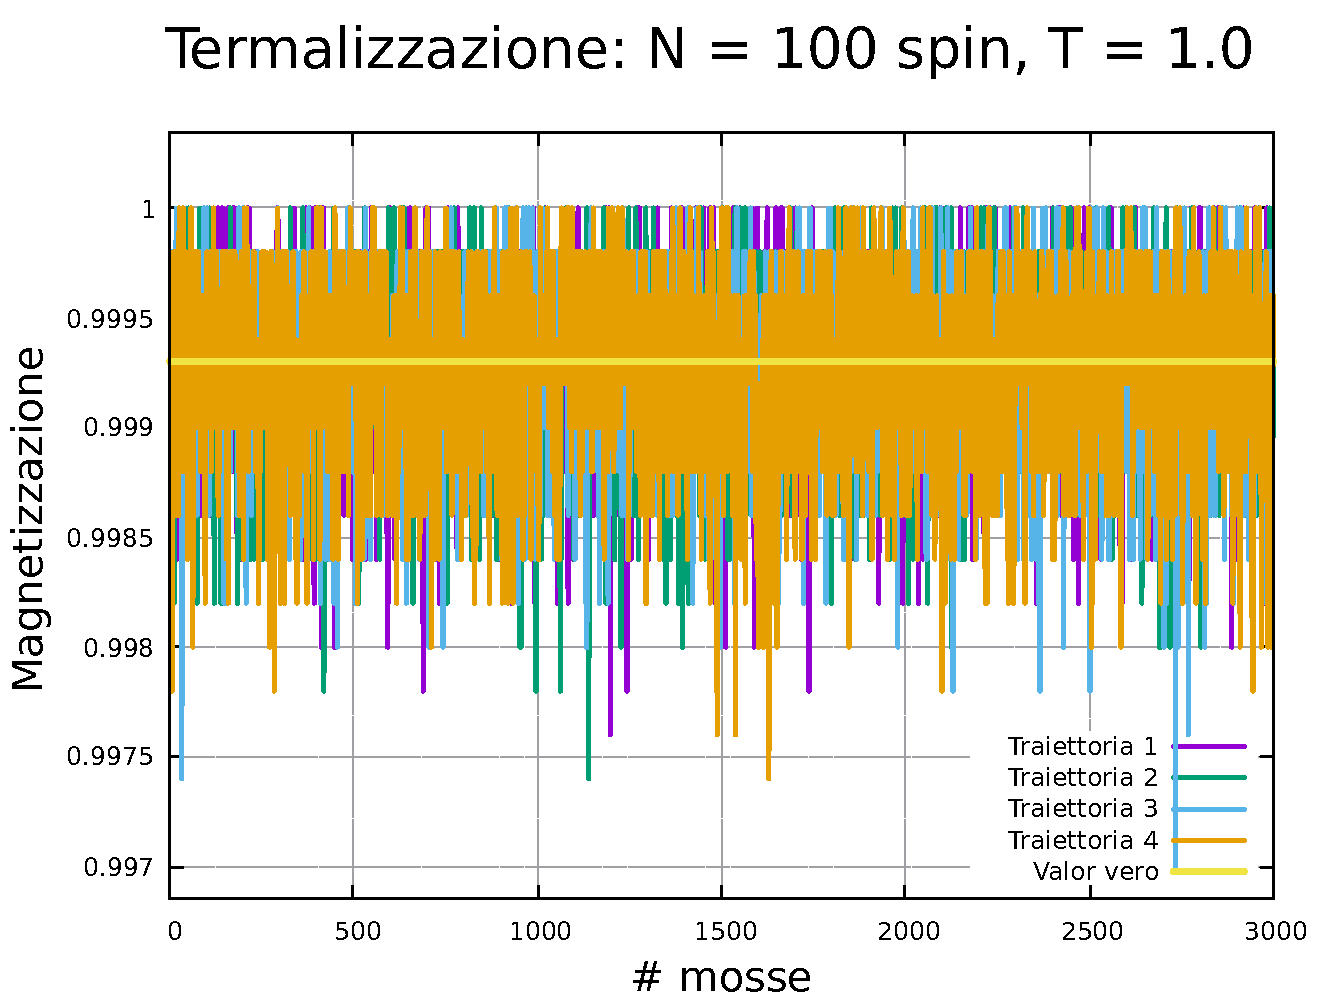
\includegraphics[page=1, width=\textwidth]{Immagini/simIsing2D/metro/term/term_100_1.0.pdf}
      \caption{$T\,=\,1.0$}
    \end{minipage}\hfill
    \begin{minipage}{0.45\textwidth}  
      \centering
      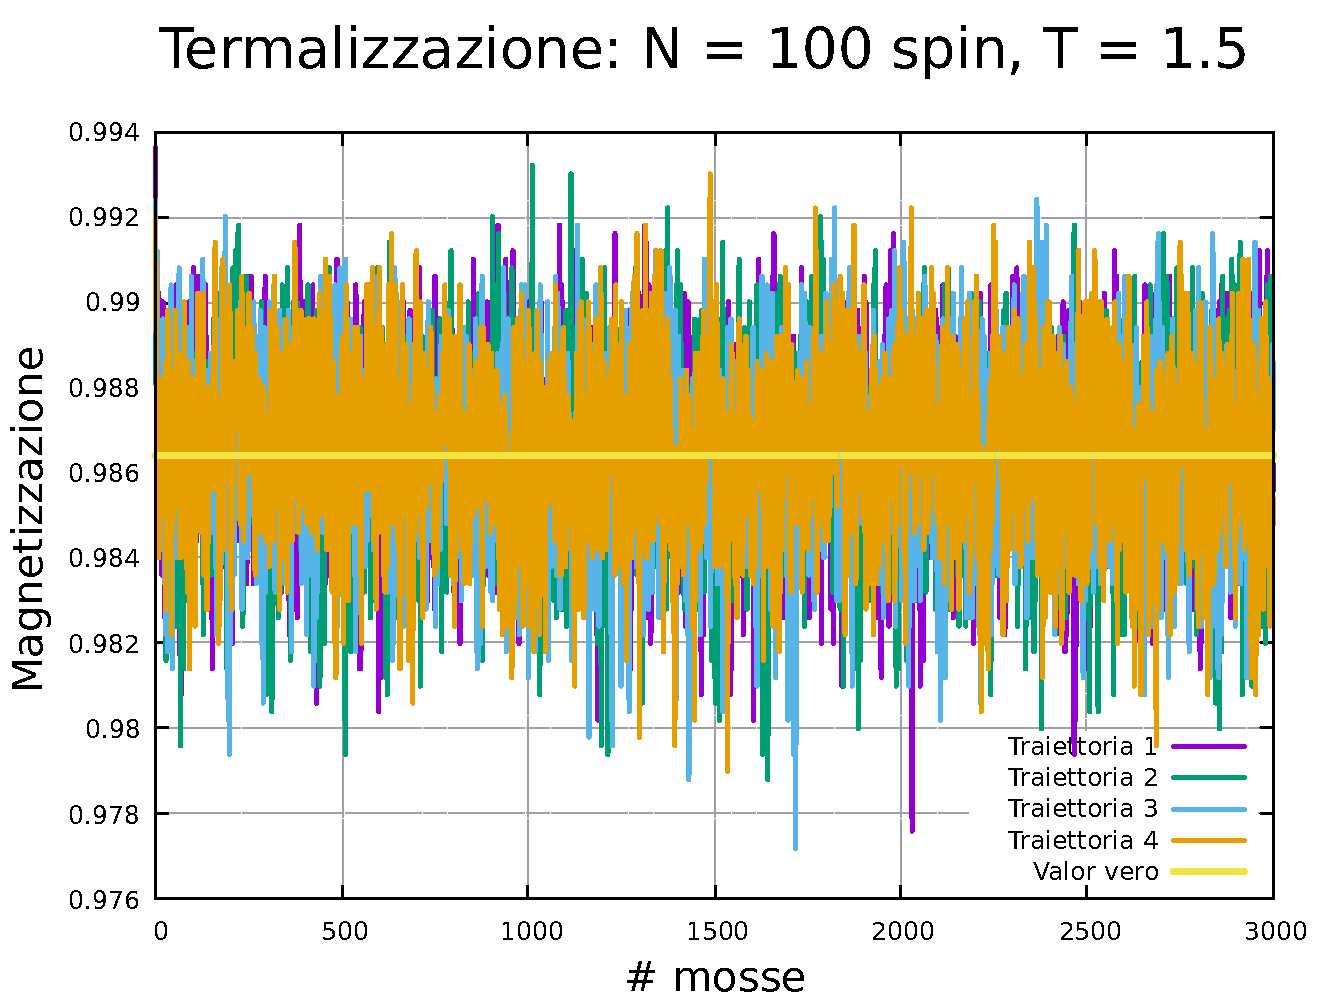
\includegraphics[page=1, width=\textwidth]{Immagini/simIsing2D/metro/term/term_100_1.5.pdf}
      \caption{$T\,=\,1.5$}
    \end{minipage}
    \vskip\baselineskip 

    \begin{minipage}{0.45\textwidth}  
        \centering
        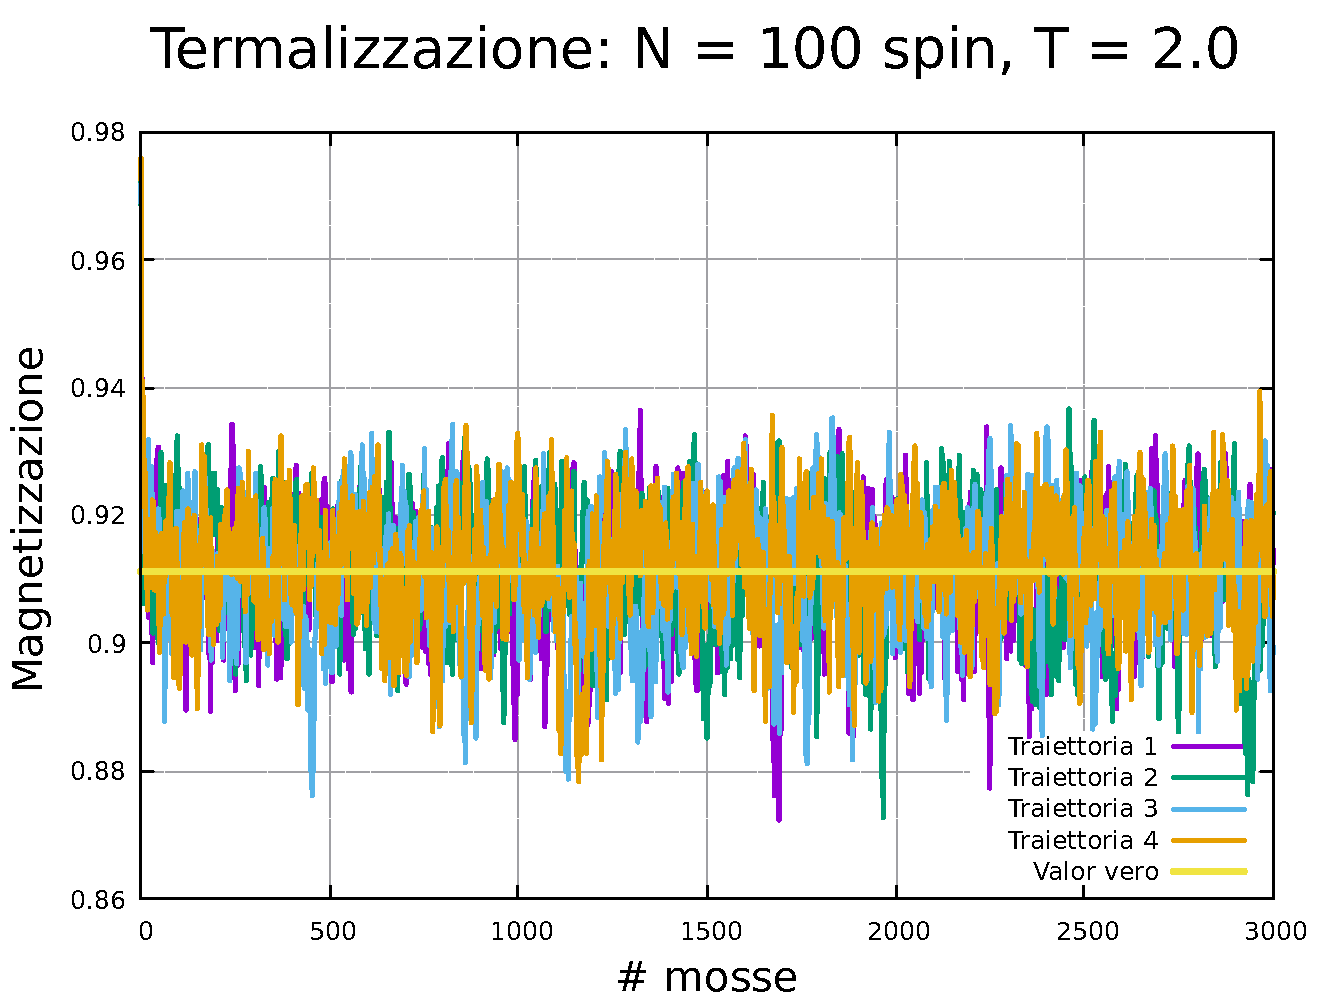
\includegraphics[page=1, width=\textwidth]{Immagini/simIsing2D/metro/term/term_100_2.0.pdf}
        \caption{$T\,=\,2.0$}
      \end{minipage}\hfill
      \begin{minipage}{0.45\textwidth}  
        \centering
        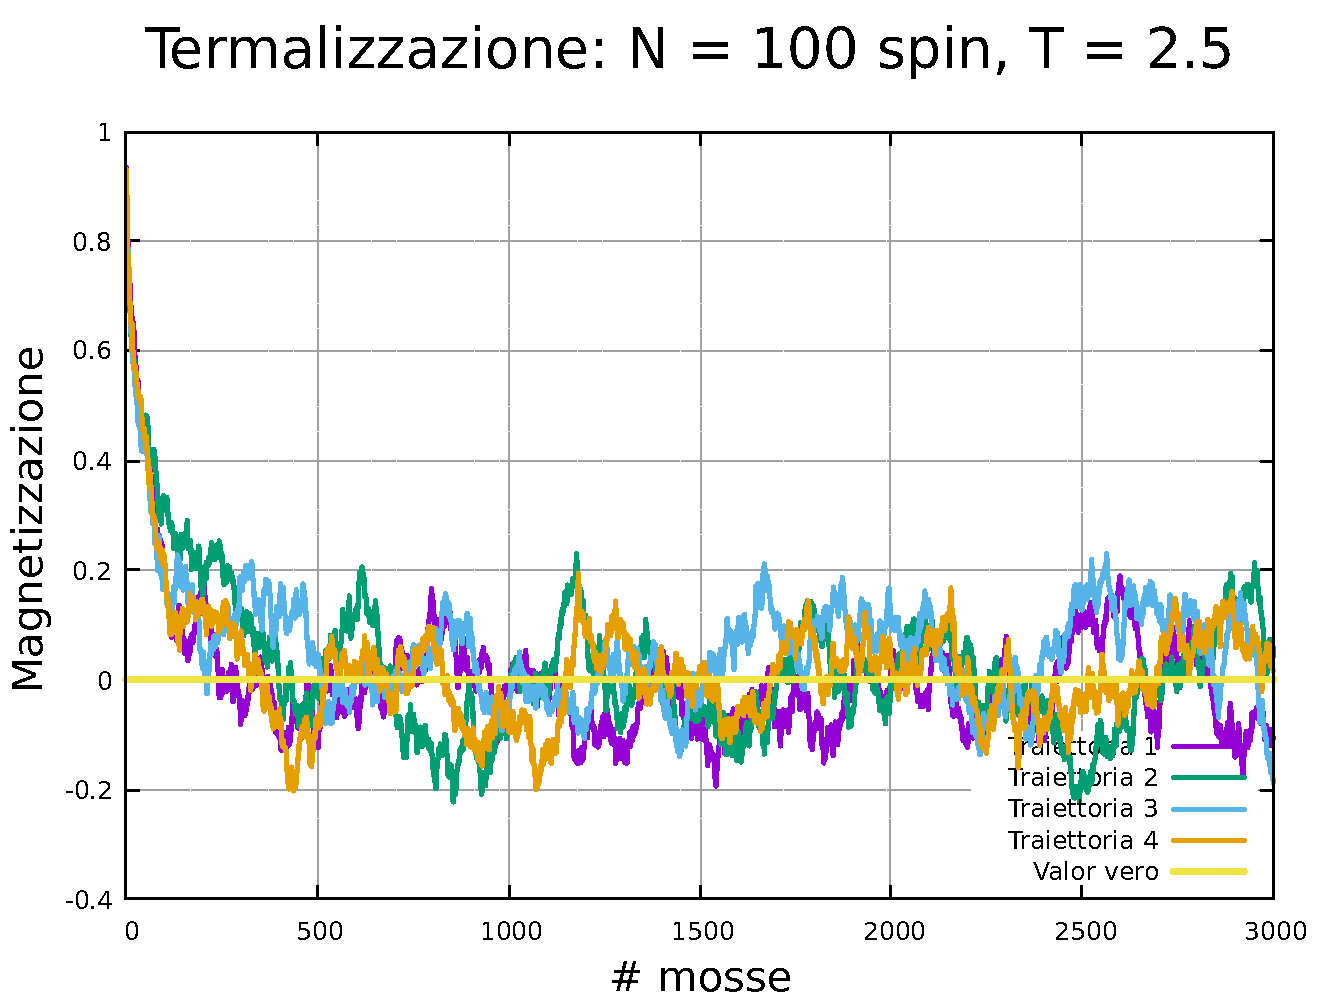
\includegraphics[page=1, width=\textwidth]{Immagini/simIsing2D/metro/term/term_100_2.5.pdf}
        \caption{$T\,=\,2.5$}
      \end{minipage}
    \vskip\baselineskip 
  
    \begin{minipage}{0.45\textwidth}  
      \centering
      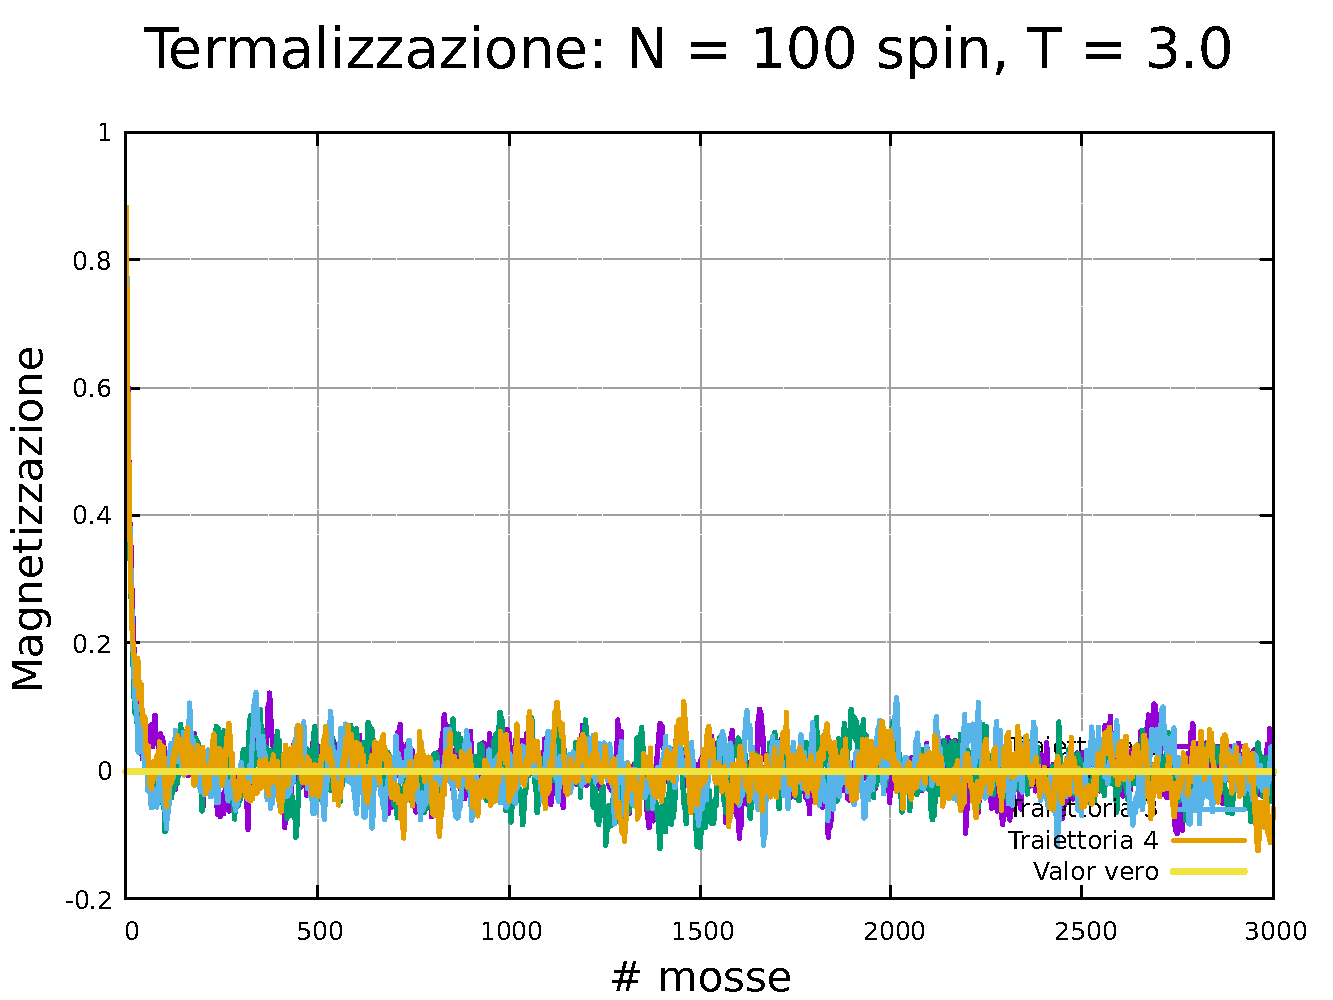
\includegraphics[page=1, width=\textwidth]{Immagini/simIsing2D/metro/term/term_100_3.0.pdf}
      \caption{$T\,=\,3.0$}
    \end{minipage}\hfill
    \begin{minipage}{0.45\textwidth}  
      \centering
      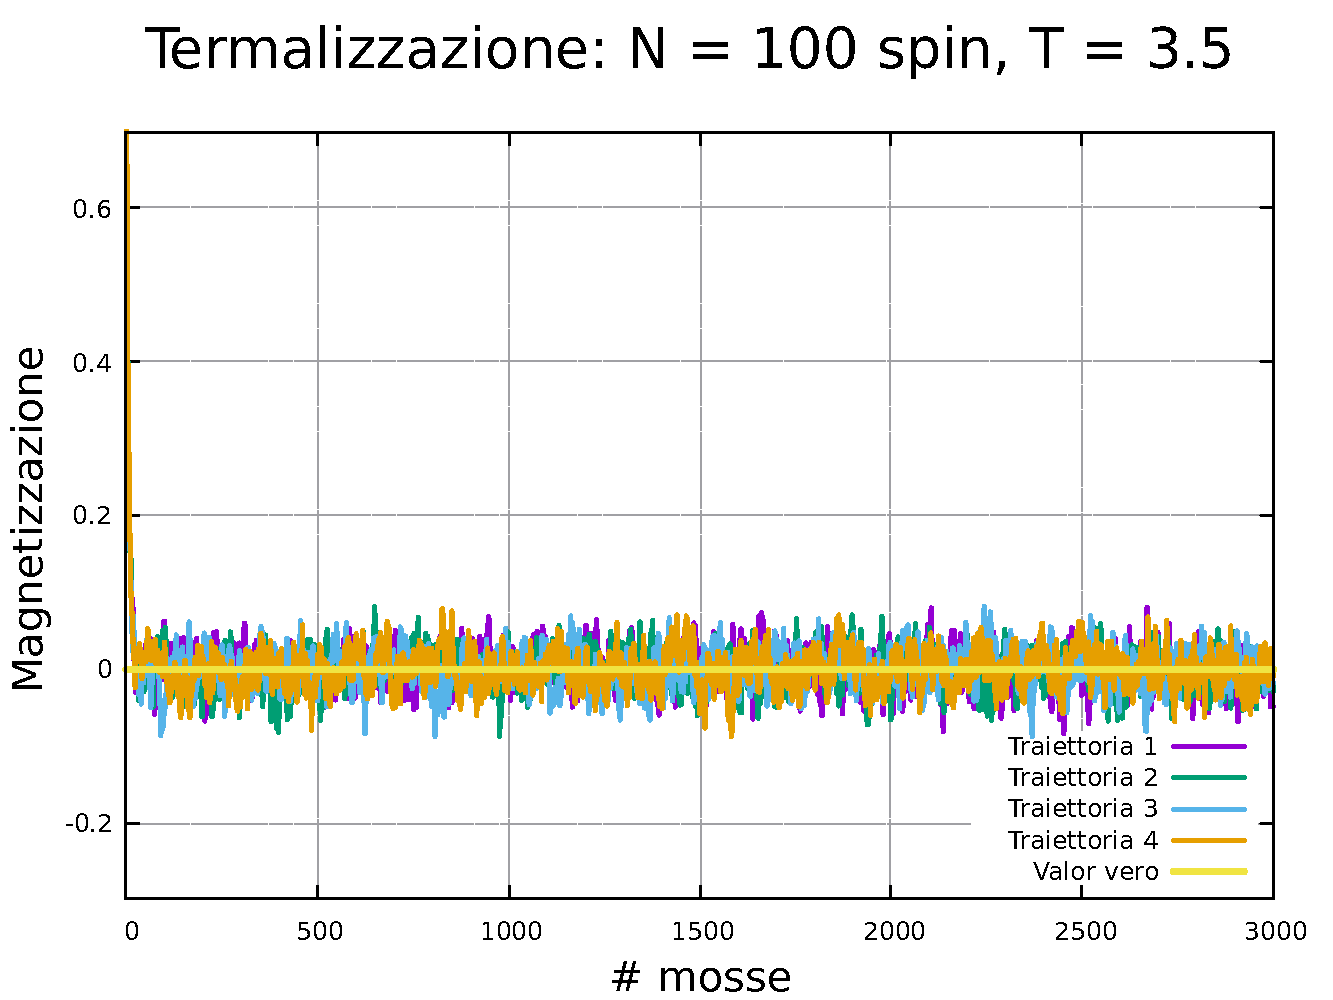
\includegraphics[page=1, width=\textwidth]{Immagini/simIsing2D/metro/term/term_100_3.5.pdf}
      \caption{$T\,=\,3.5$}
    \end{minipage}
    \caption{Studio della termalizzazione di un modello di Ising 2D costituito da $100 \times 100$ spin.}
\end{figure}

\vspace*{\fill}



\vspace*{\fill}

\begin{figure}[H]
    \centering
    \begin{minipage}{0.45\textwidth}  
      \centering
      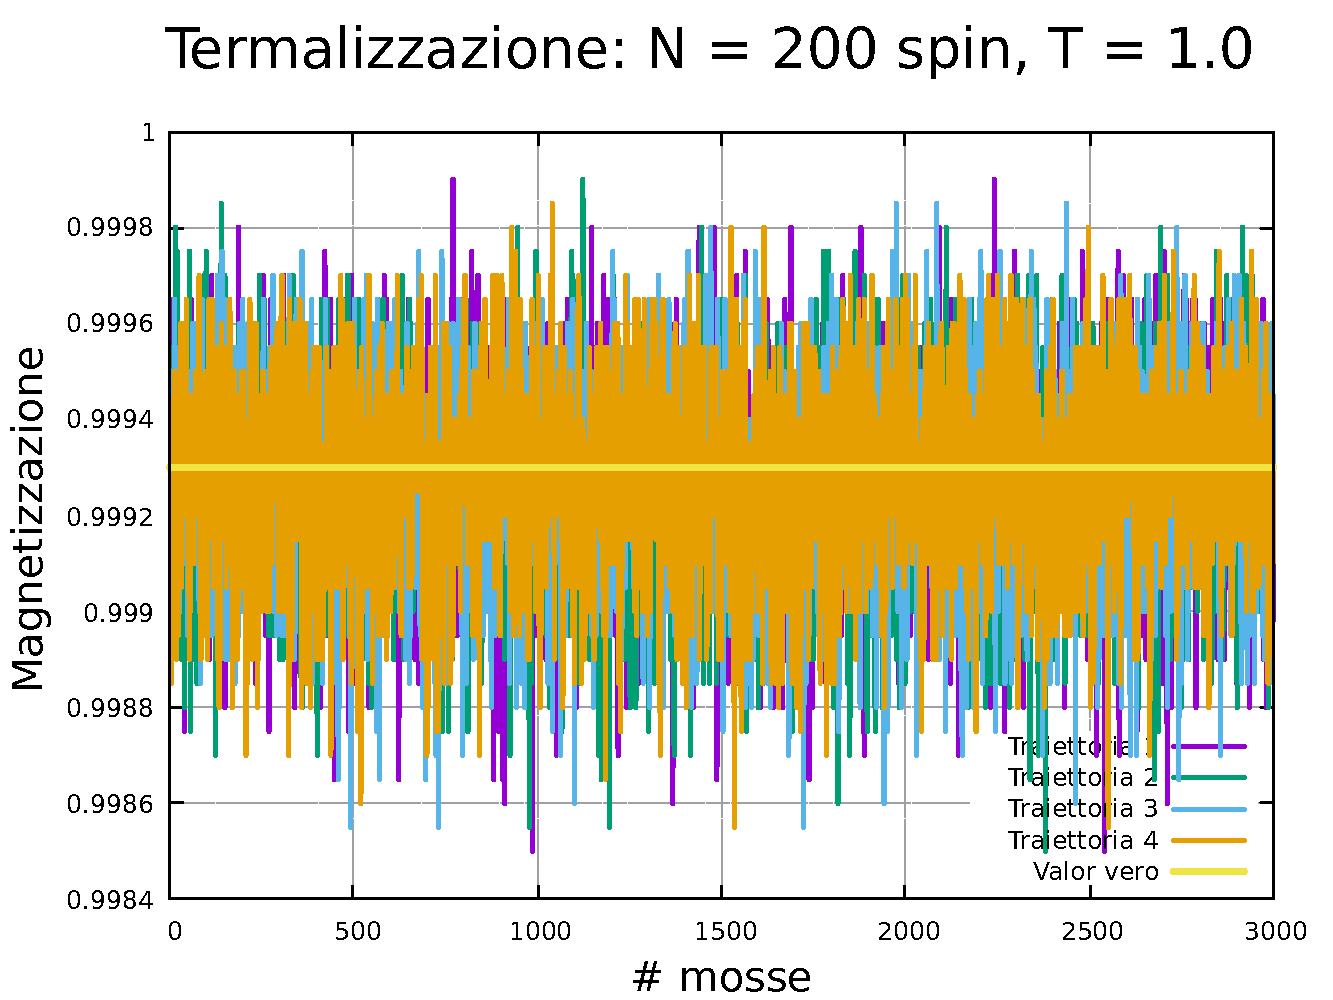
\includegraphics[page=1, width=\textwidth]{Immagini/simIsing2D/metro/term/term_200_1.0.pdf}
      \caption{$T\,=\,1.0$}
    \end{minipage}\hfill
    \begin{minipage}{0.45\textwidth}  
      \centering
      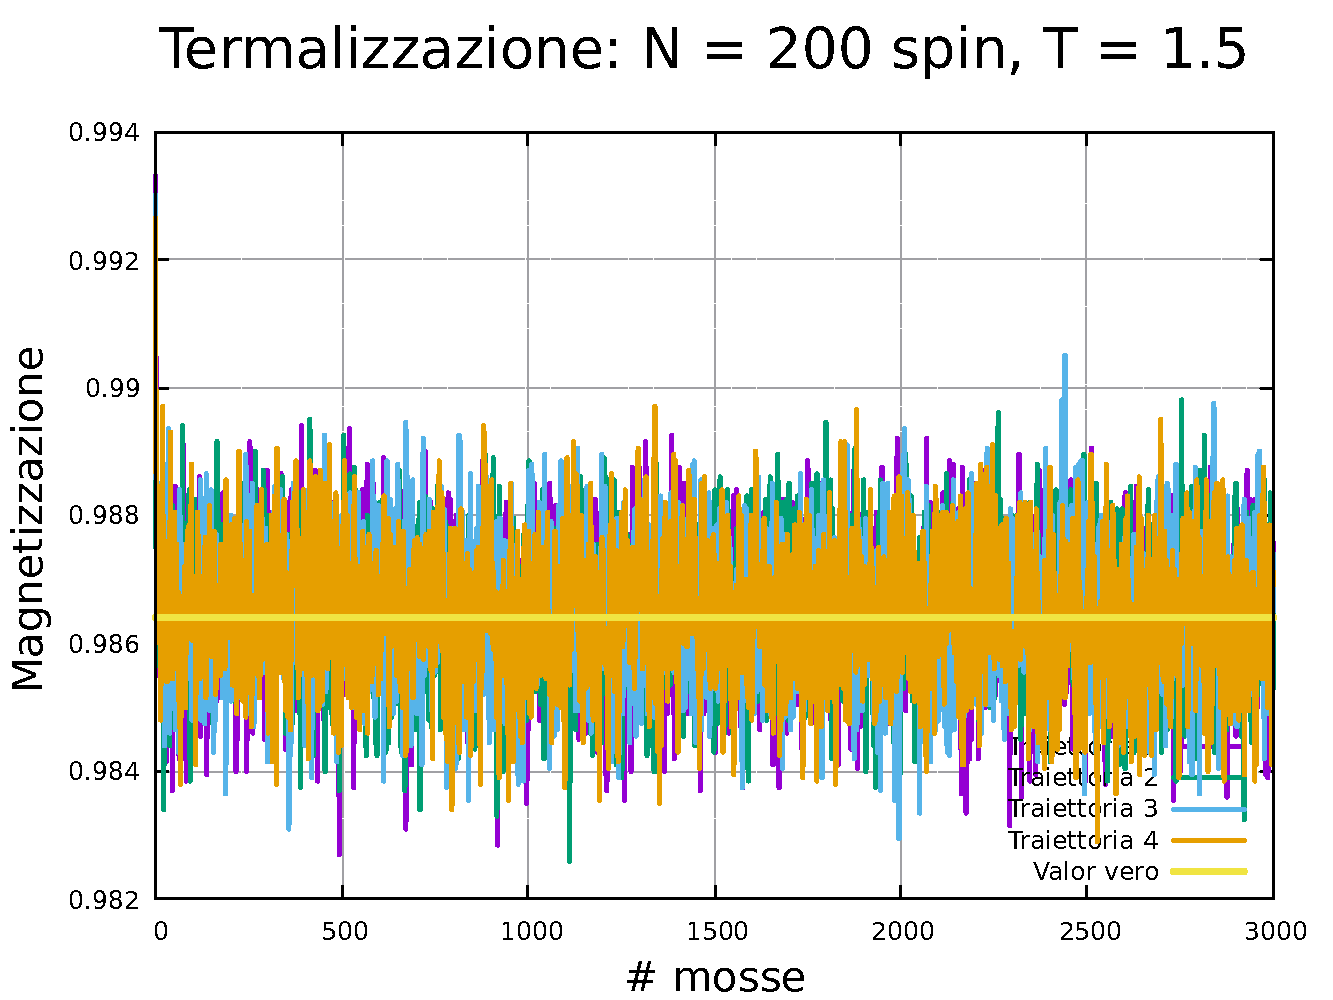
\includegraphics[page=1, width=\textwidth]{Immagini/simIsing2D/metro/term/term_200_1.5.pdf}
      \caption{$T\,=\,1.5$}
    \end{minipage}
    \vskip\baselineskip 
  
    \begin{minipage}{0.45\textwidth}  
      \centering
      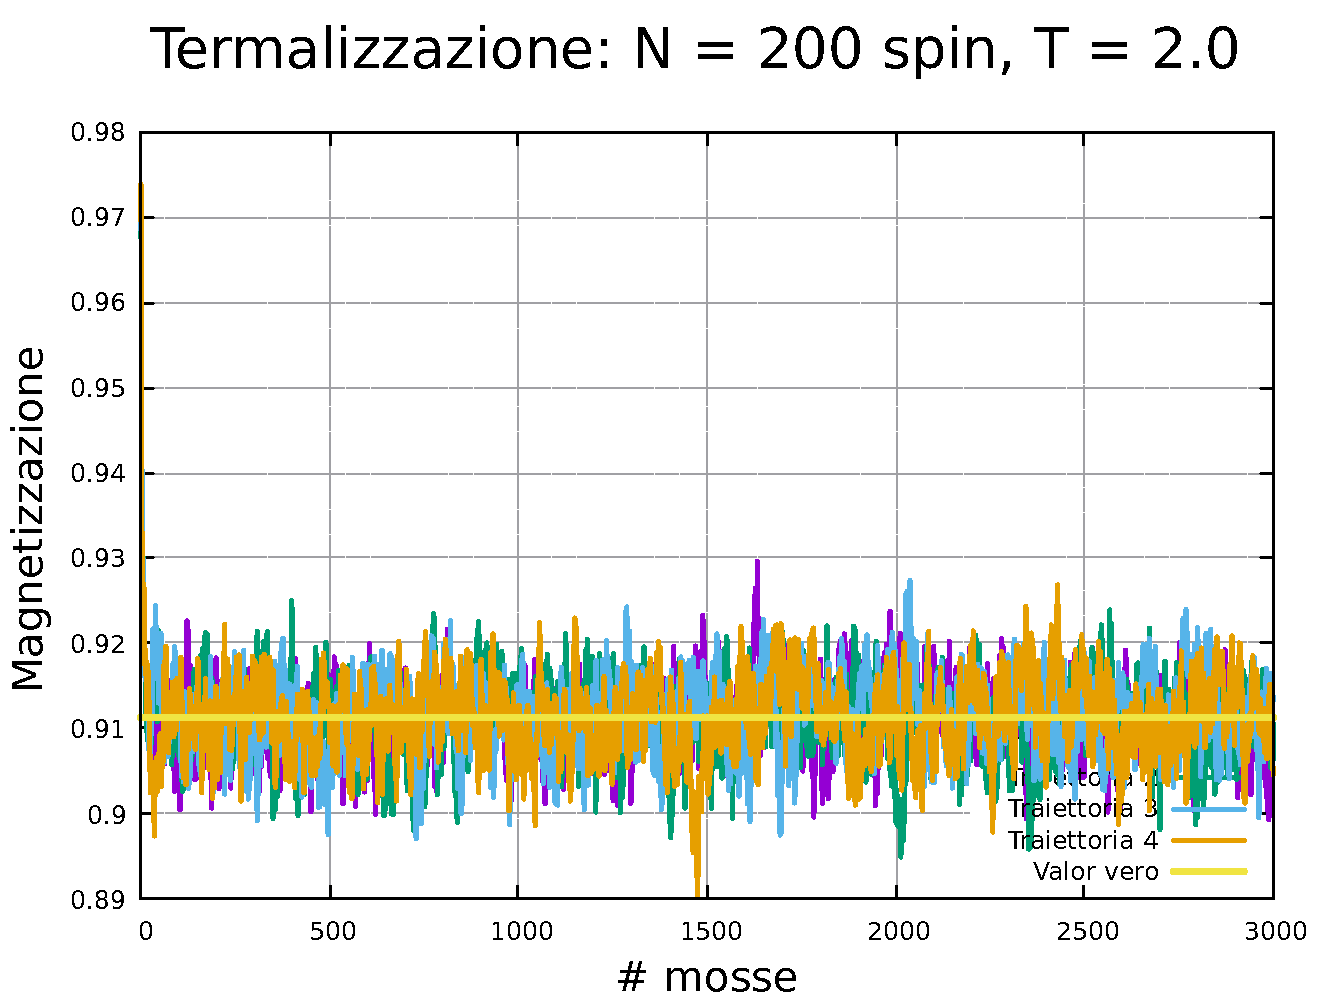
\includegraphics[page=1, width=\textwidth]{Immagini/simIsing2D/metro/term/term_200_2.0.pdf}
      \caption{$T\,=\,2.0$}
    \end{minipage}\hfill
    \begin{minipage}{0.45\textwidth}  
      \centering
      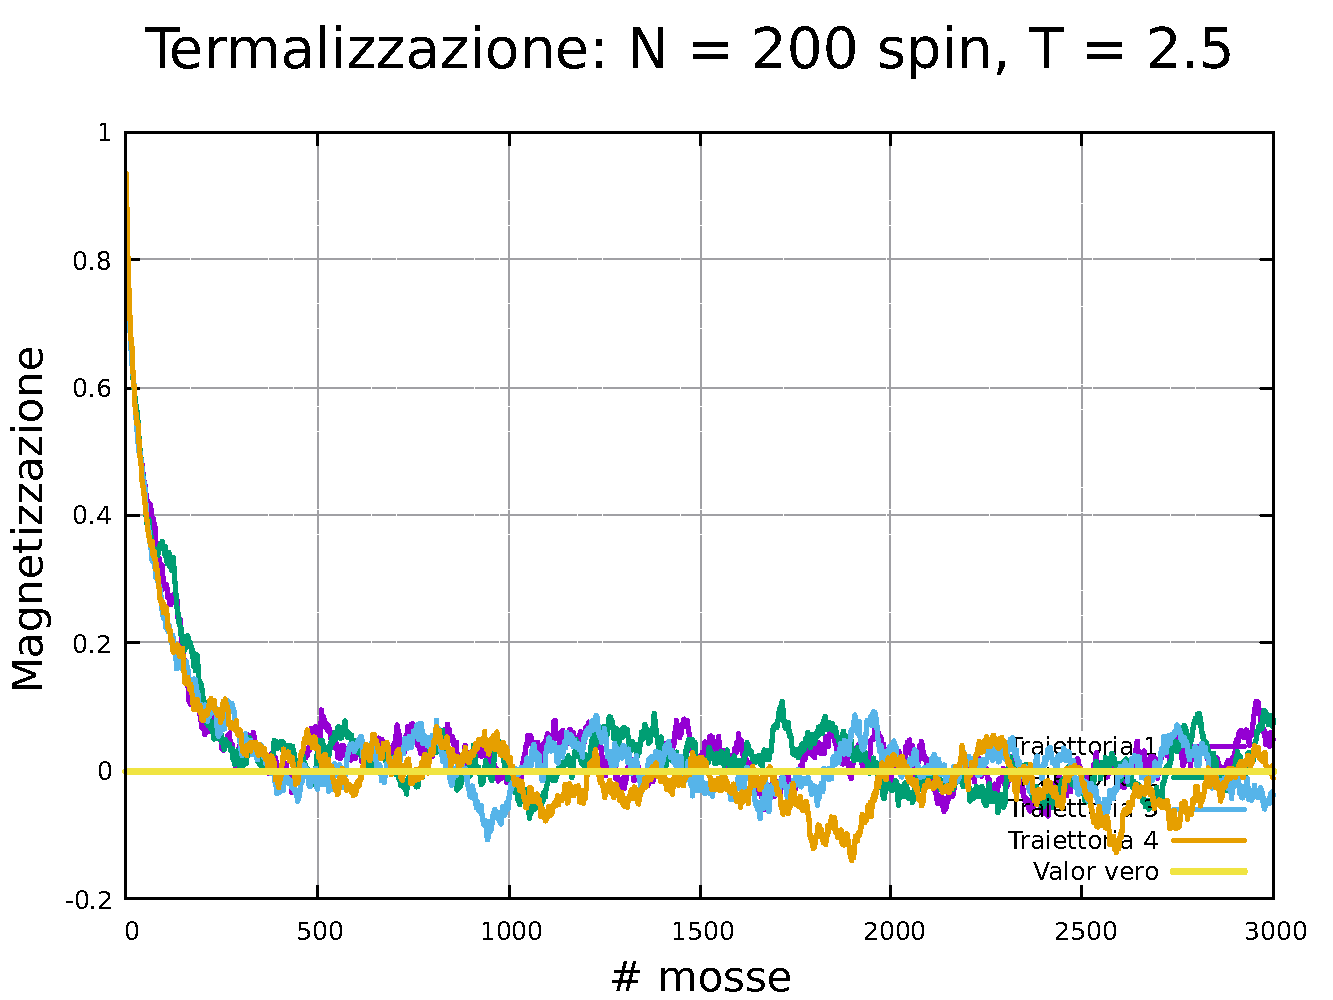
\includegraphics[page=1, width=\textwidth]{Immagini/simIsing2D/metro/term/term_200_2.5.pdf}
      \caption{$T\,=\,2.5$}
    \end{minipage}
    \vskip\baselineskip 

    \begin{minipage}{0.45\textwidth}  
        \centering
        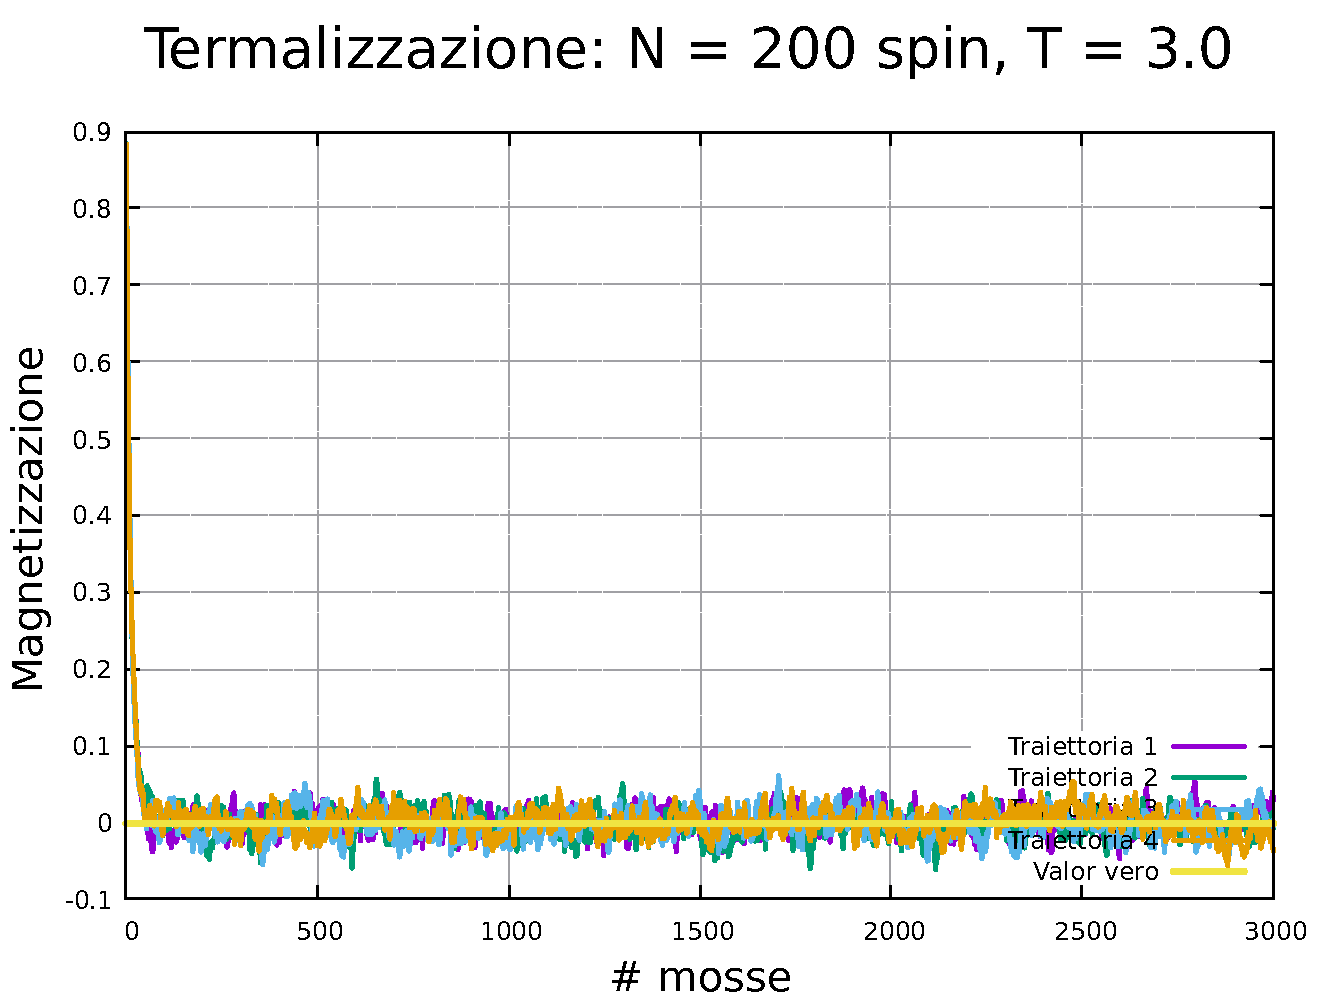
\includegraphics[page=1, width=\textwidth]{Immagini/simIsing2D/metro/term/term_200_3.0.pdf}
        \caption{$T\,=\,3.0$}
      \end{minipage}\hfill
      \begin{minipage}{0.45\textwidth}  
        \centering
        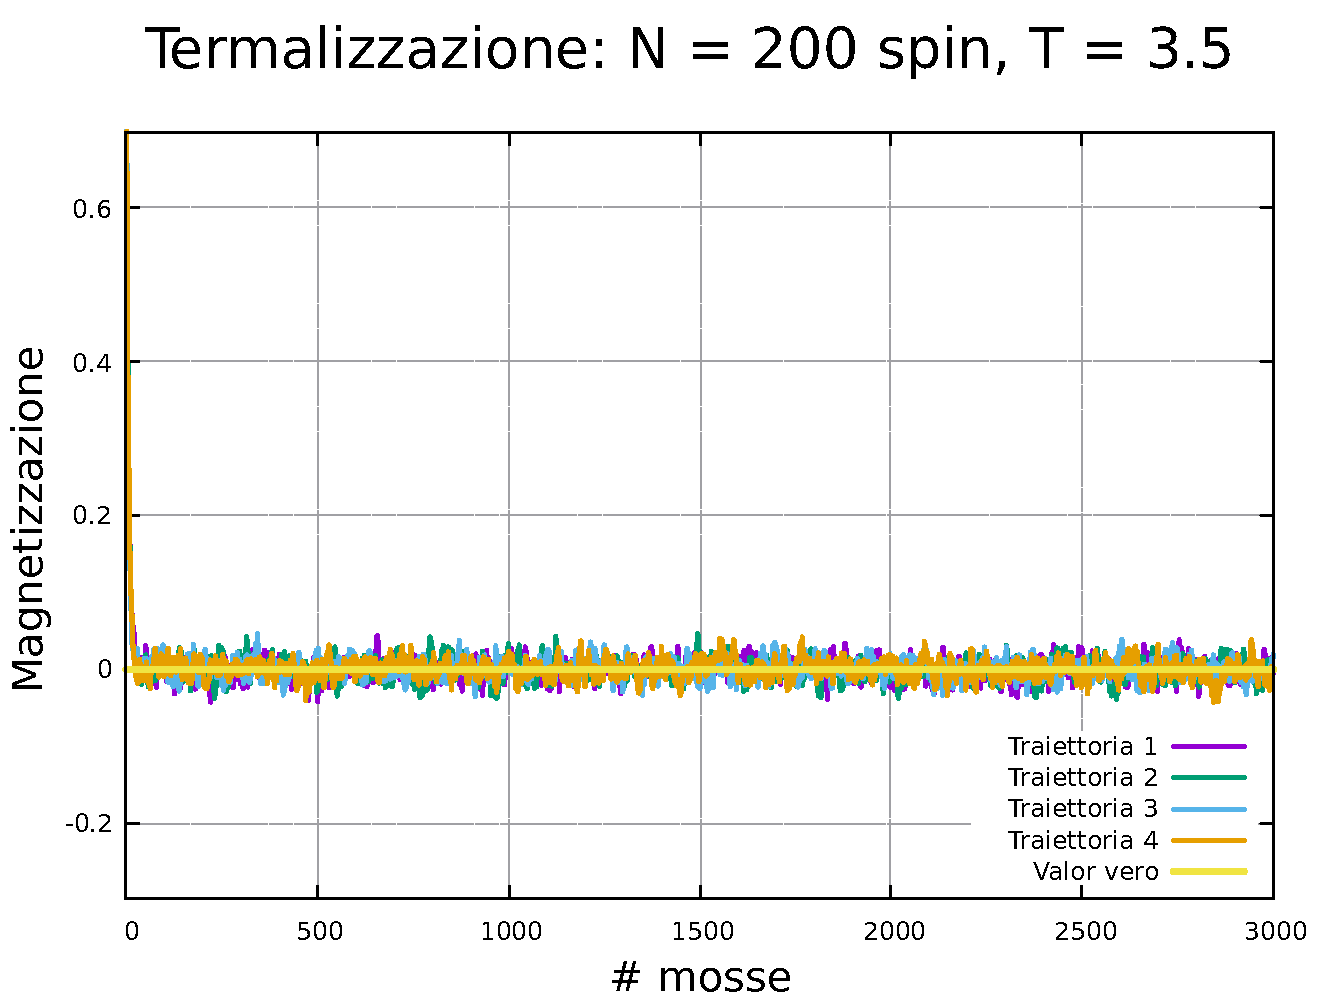
\includegraphics[page=1, width=\textwidth]{Immagini/simIsing2D/metro/term/term_200_3.5.pdf}
        \caption{$T\,=\,3.5$}
    \end{minipage}

    \caption{Studio della termalizzazione di un modello di Ising 2D costituito da $200 \times 200$ spin.}
\end{figure}

\vspace*{\fill}



\vspace*{\fill}

\begin{figure}[H]
    \centering
    \begin{minipage}{0.45\textwidth}  
      \centering
      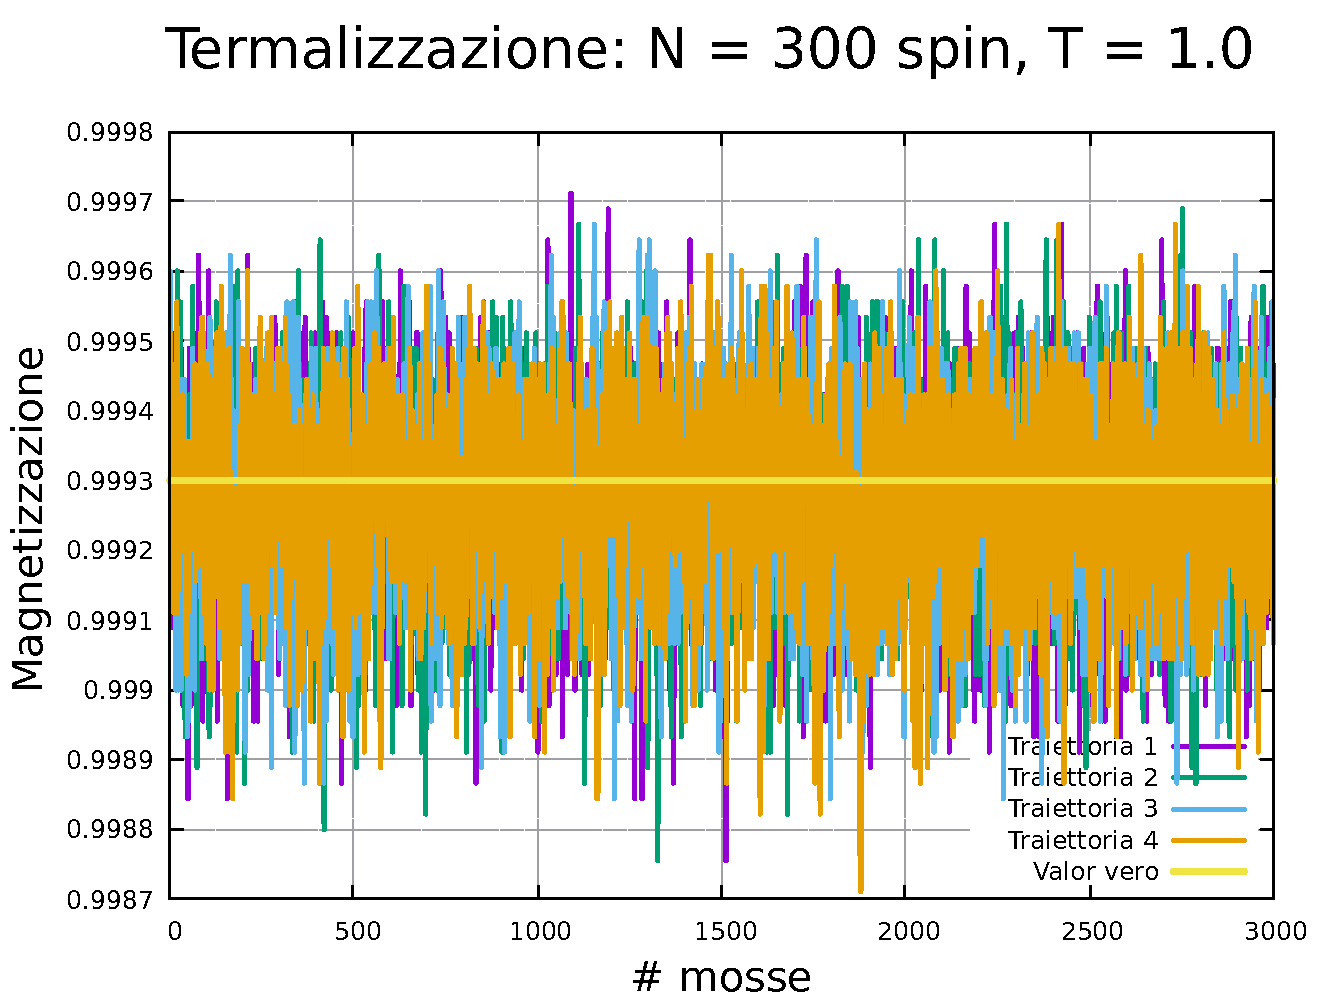
\includegraphics[page=1, width=\textwidth]{Immagini/simIsing2D/metro/term/term_300_1.0.pdf}
      \caption{$T\,=\,1.0$}
    \end{minipage}\hfill
    \begin{minipage}{0.45\textwidth}  
      \centering
      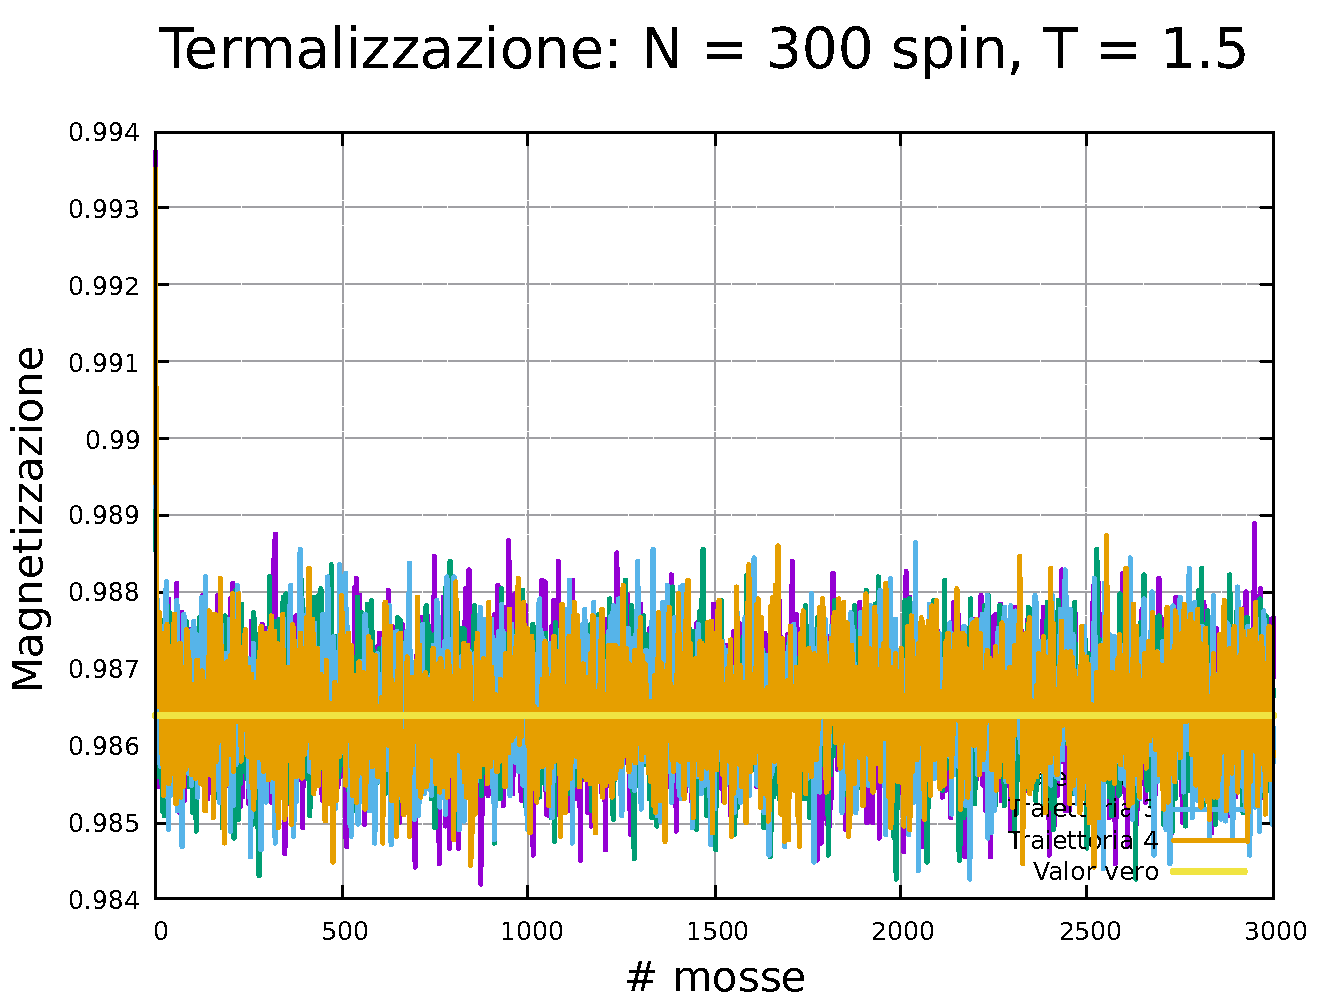
\includegraphics[page=1, width=\textwidth]{Immagini/simIsing2D/metro/term/term_300_1.5.pdf}
      \caption{$T\,=\,1.5$}
    \end{minipage}
    \vskip\baselineskip 

    \begin{minipage}{0.45\textwidth}  
        \centering
        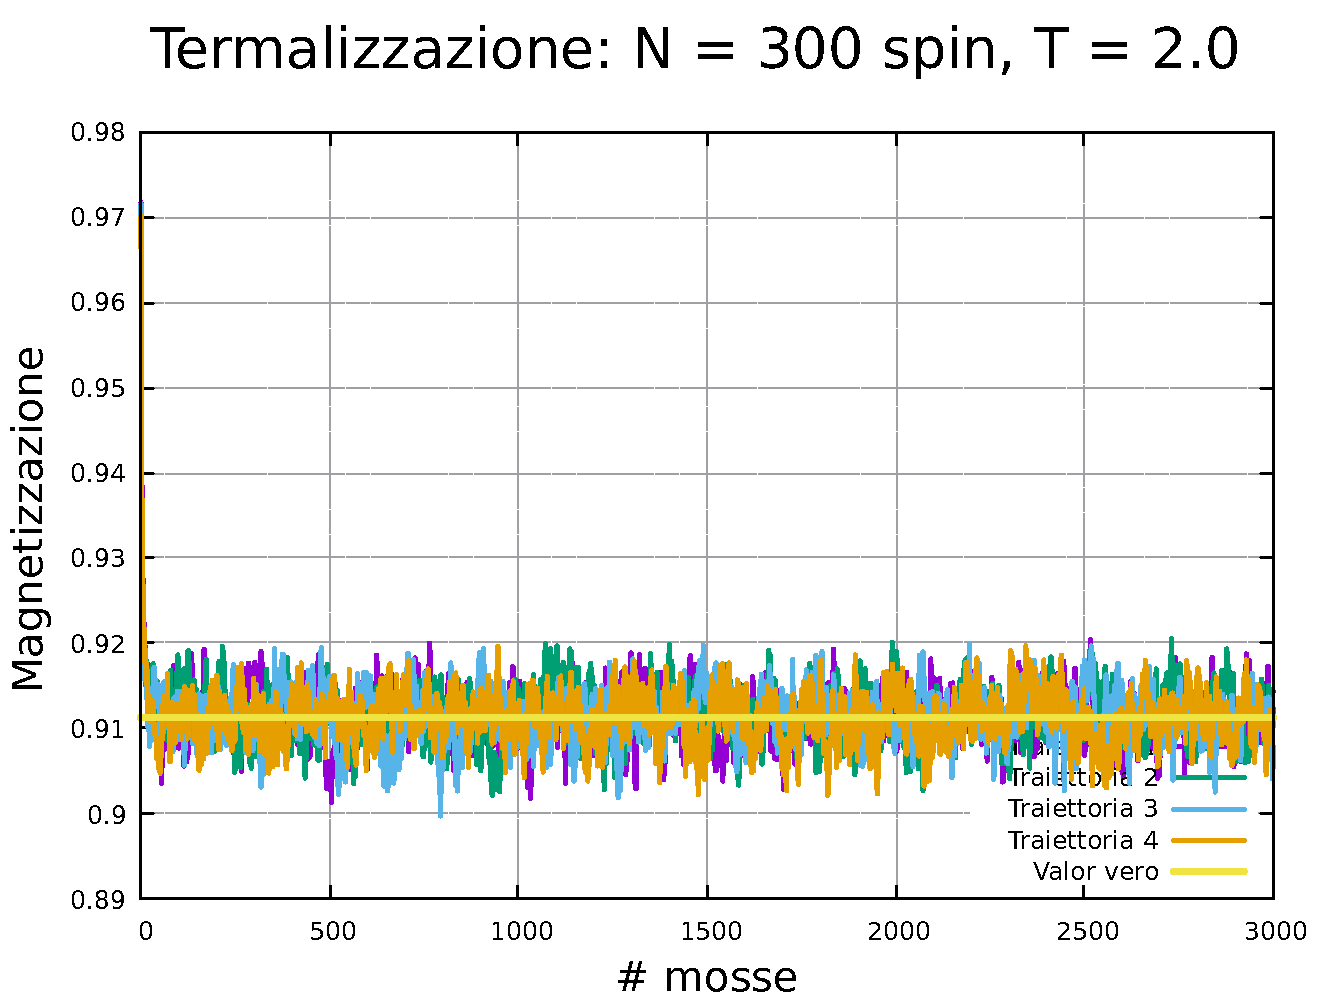
\includegraphics[page=1, width=\textwidth]{Immagini/simIsing2D/metro/term/term_300_2.0.pdf}
        \caption{$T\,=\,2.0$}
      \end{minipage}\hfill
      \begin{minipage}{0.45\textwidth}  
        \centering
        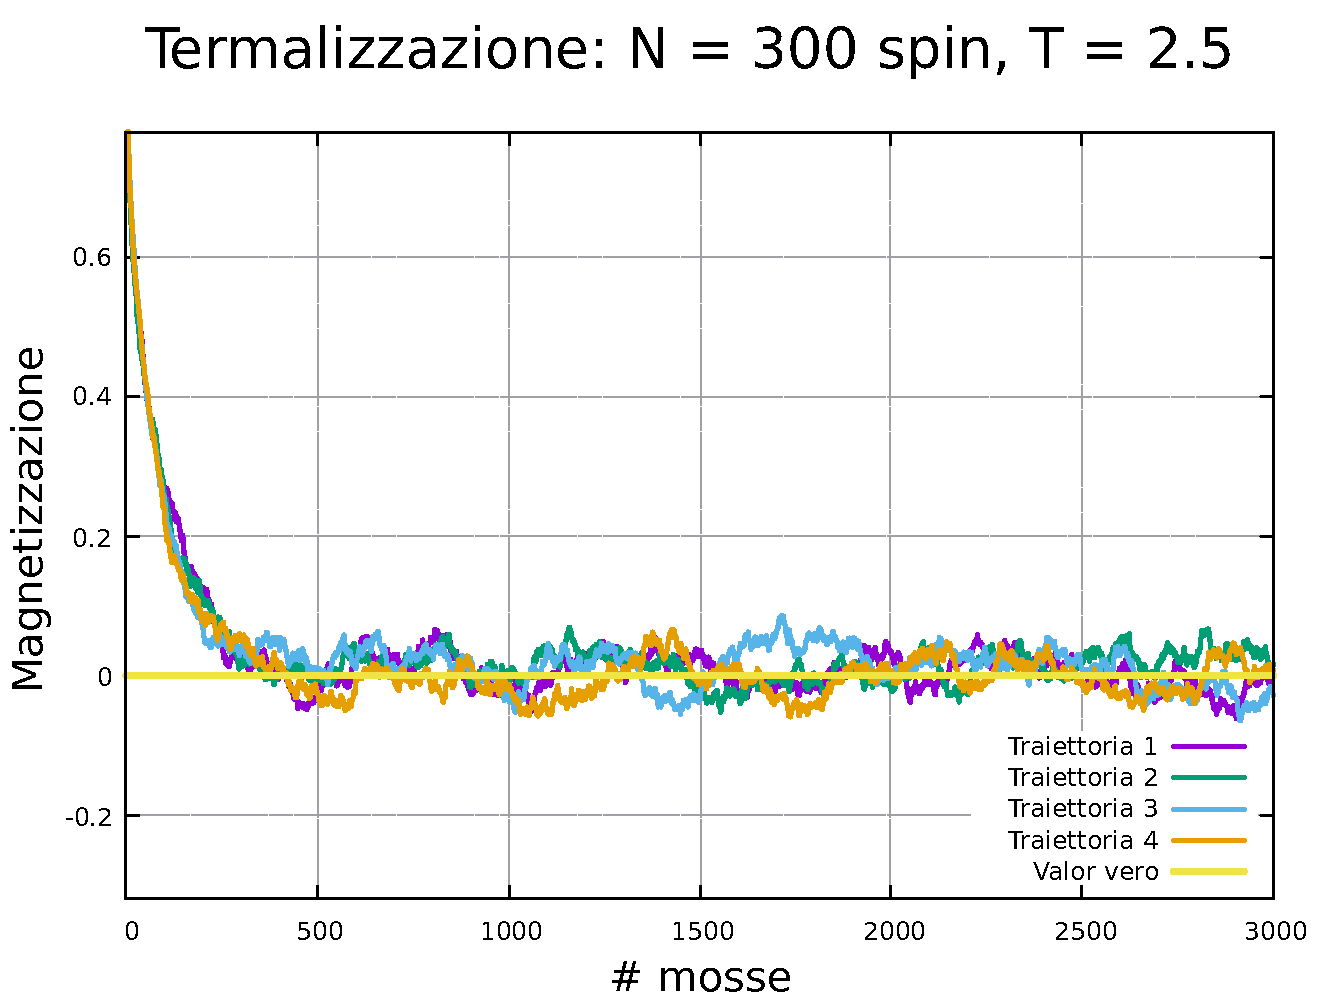
\includegraphics[page=1, width=\textwidth]{Immagini/simIsing2D/metro/term/term_300_2.5.pdf}
        \caption{$T\,=\,2.5$}
      \end{minipage}
    \vskip\baselineskip 
  
    \begin{minipage}{0.45\textwidth}  
      \centering
      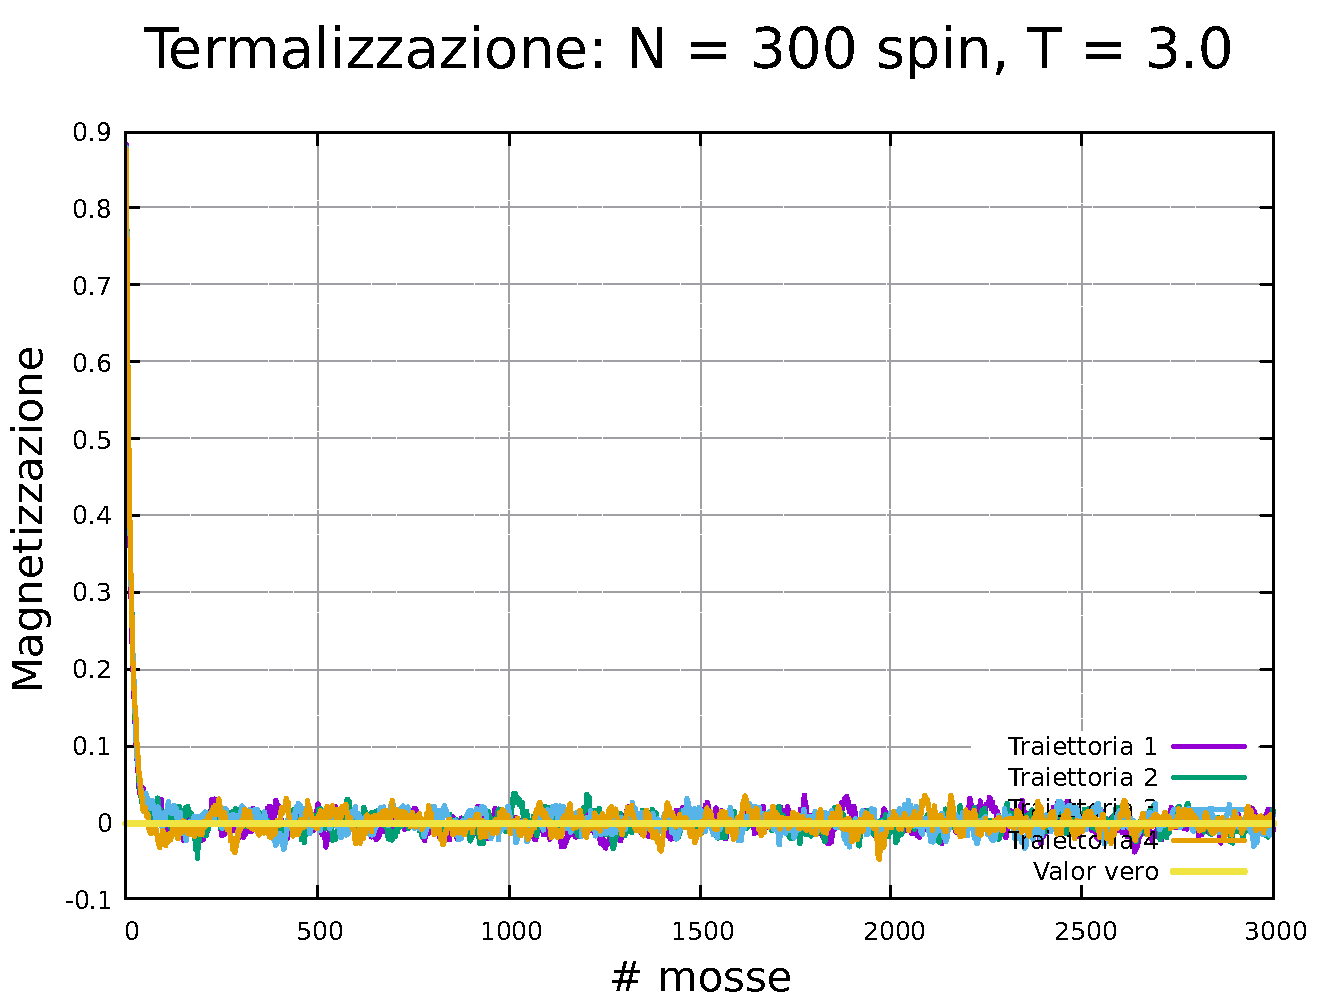
\includegraphics[page=1, width=\textwidth]{Immagini/simIsing2D/metro/term/term_300_3.0.pdf}
      \caption{$T\,=\,3.0$}
    \end{minipage}\hfill
    \begin{minipage}{0.45\textwidth}  
      \centering
      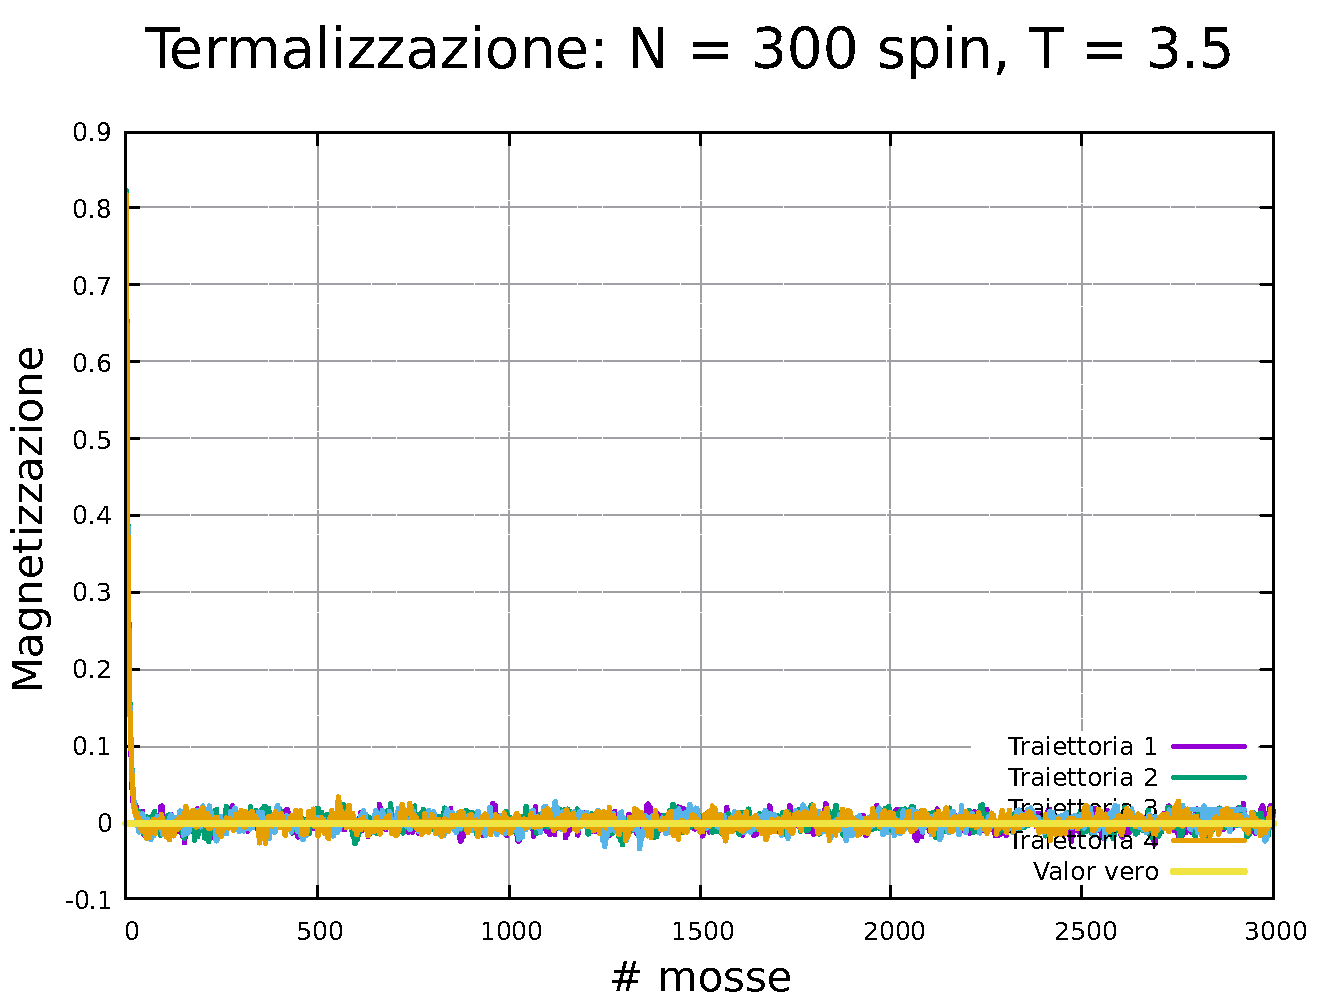
\includegraphics[page=1, width=\textwidth]{Immagini/simIsing2D/metro/term/term_300_3.5.pdf}
      \caption{$T\,=\,3.5$}
    \end{minipage}
    \caption{Studio della termalizzazione di un modello di Ising 2D costituito da $300 \times 300$ spin.}
\end{figure}

\vspace*{\fill}



\vspace*{\fill}

\begin{figure}[H]
    \centering
    \begin{minipage}{0.45\textwidth}  
      \centering
      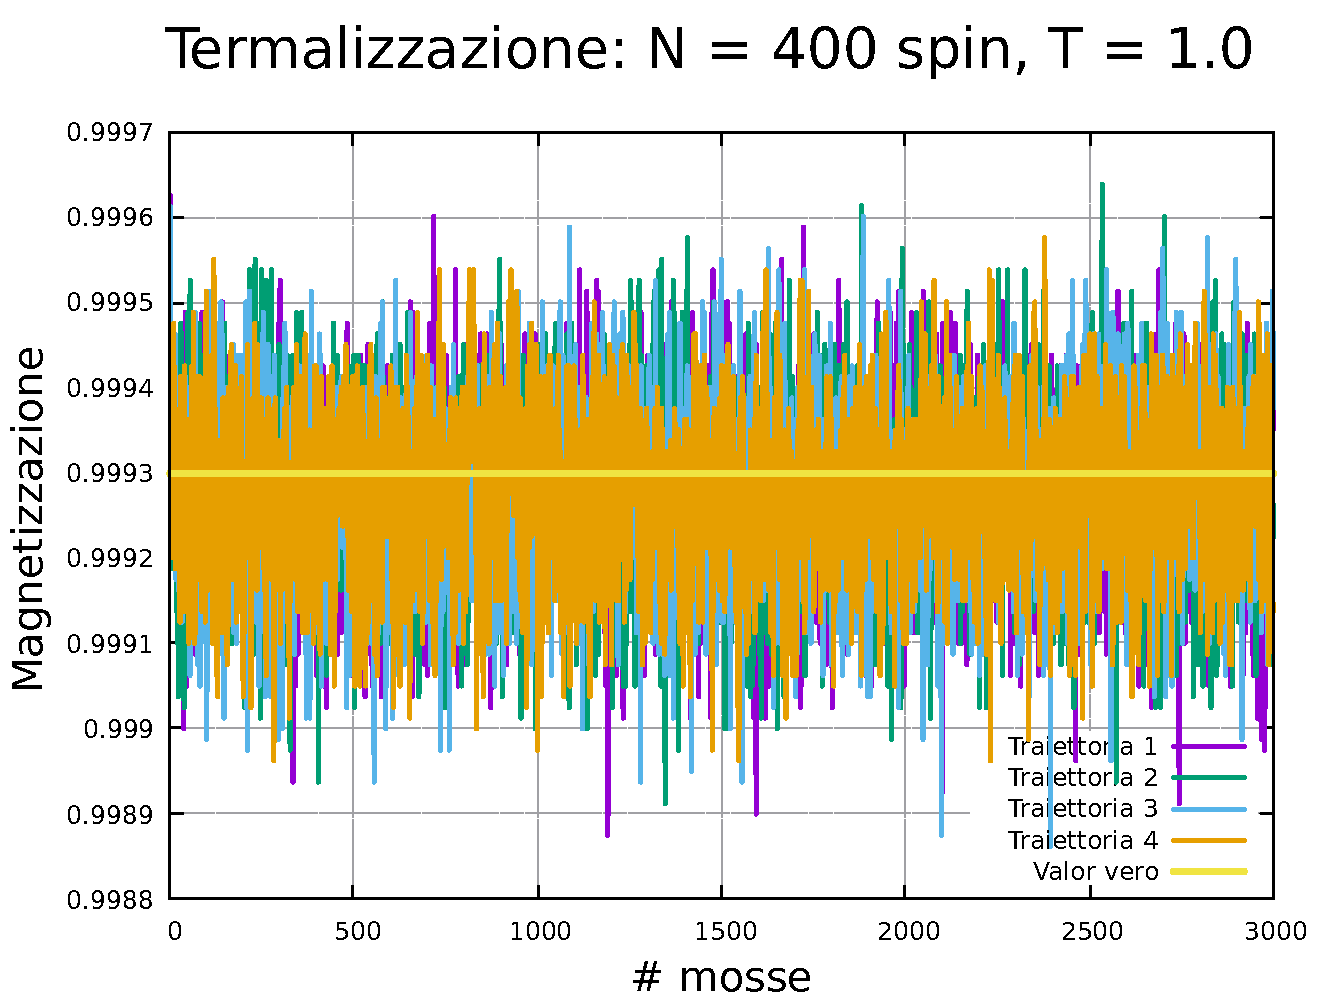
\includegraphics[page=1, width=\textwidth]{Immagini/simIsing2D/metro/term/term_400_1.0.pdf}
      \caption{$T\,=\,1.0$}
    \end{minipage}\hfill
    \begin{minipage}{0.45\textwidth}  
      \centering
      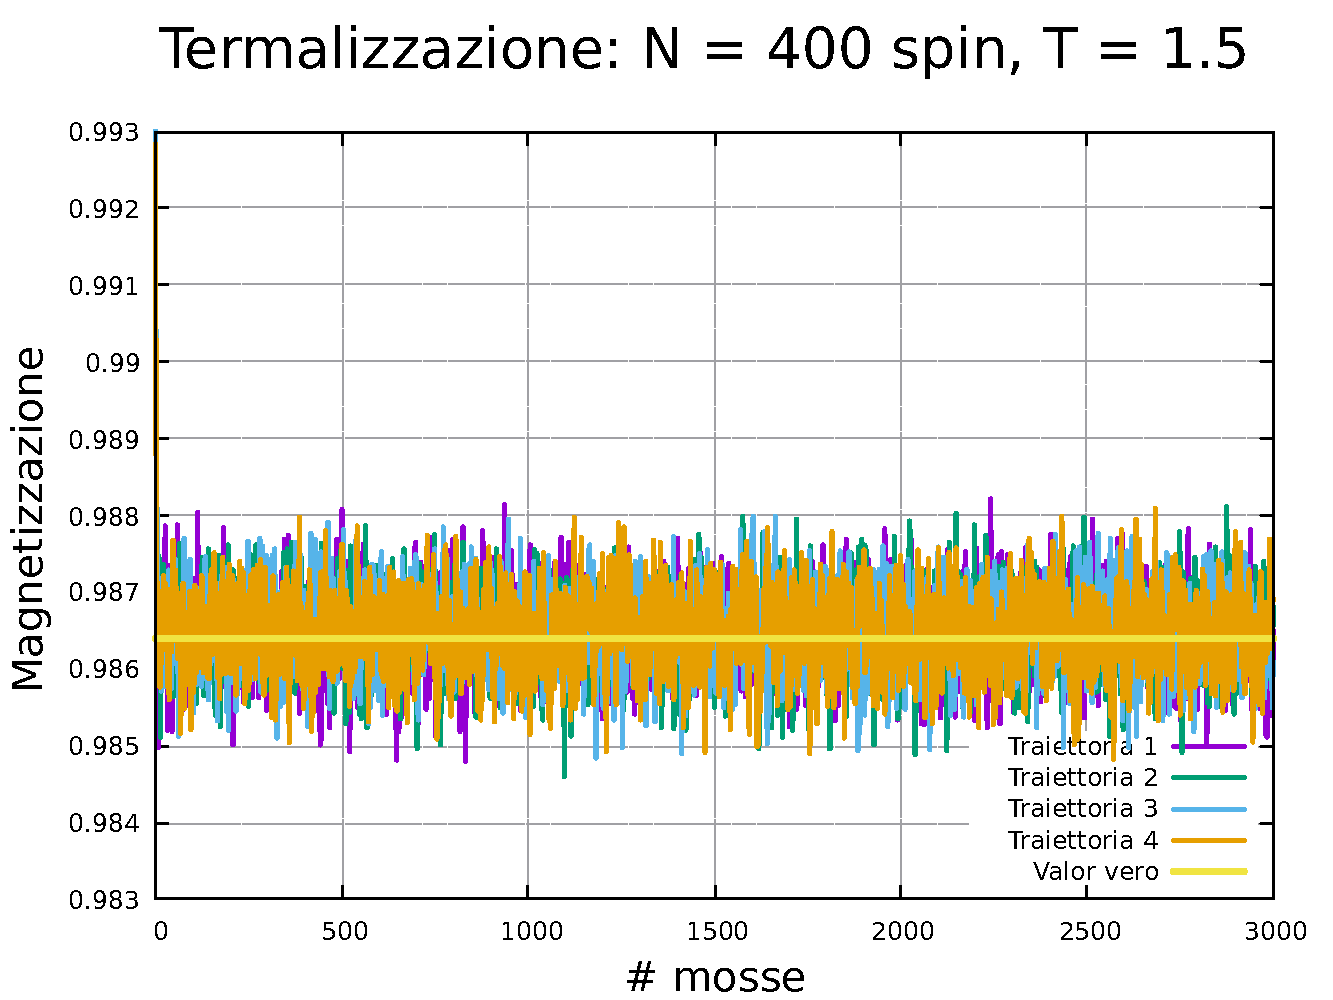
\includegraphics[page=1, width=\textwidth]{Immagini/simIsing2D/metro/term/term_400_1.5.pdf}
      \caption{$T\,=\,1.5$}
    \end{minipage}
    \vskip\baselineskip 

    \begin{minipage}{0.45\textwidth}  
        \centering
        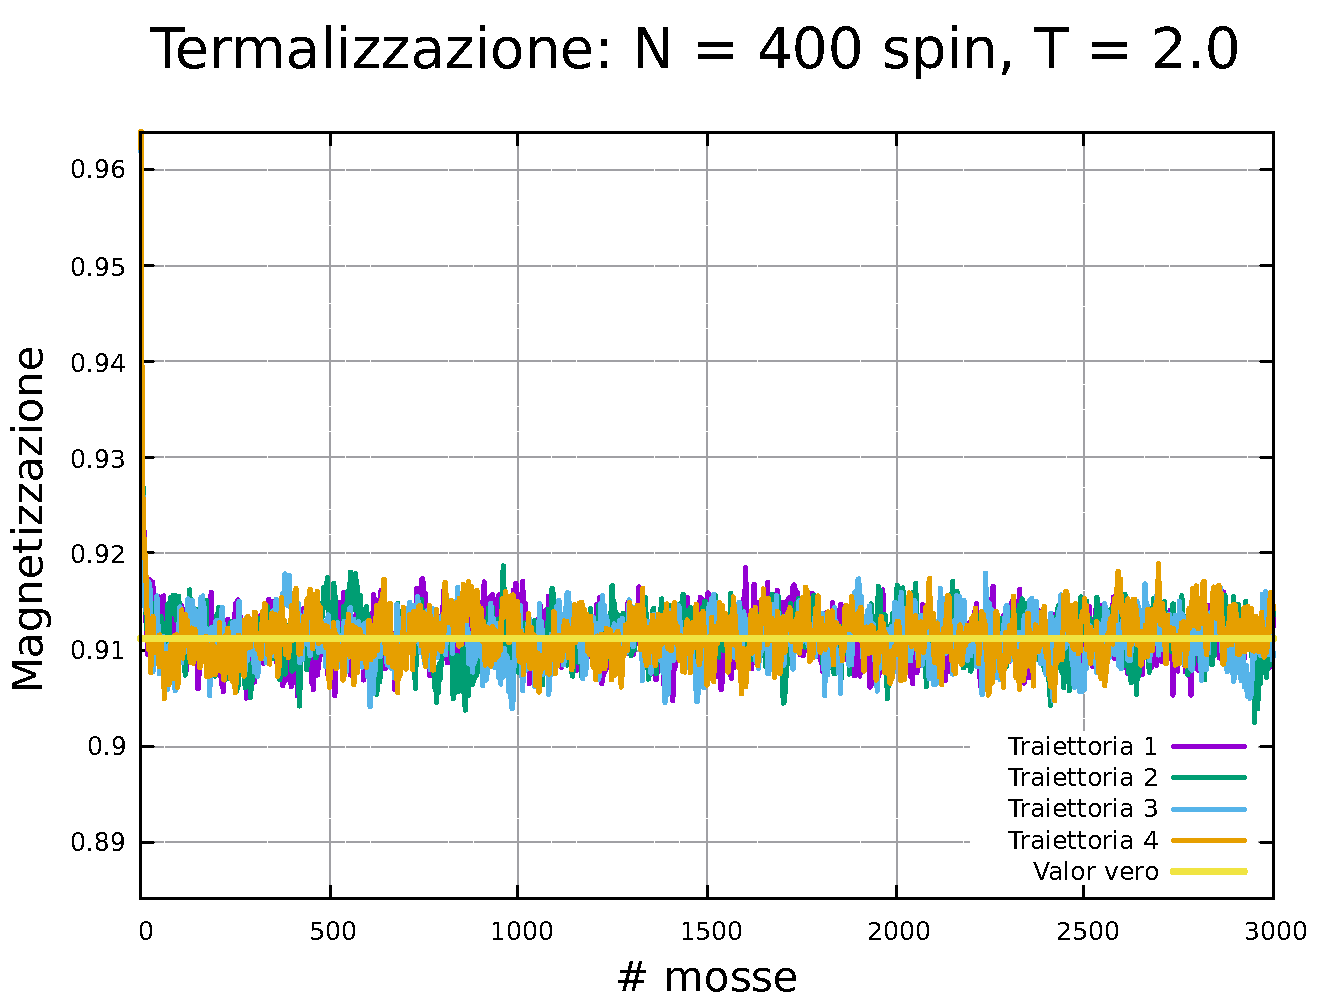
\includegraphics[page=1, width=\textwidth]{Immagini/simIsing2D/metro/term/term_400_2.0.pdf}
        \caption{$T\,=\,2.0$}
      \end{minipage}\hfill
      \begin{minipage}{0.45\textwidth}  
        \centering
        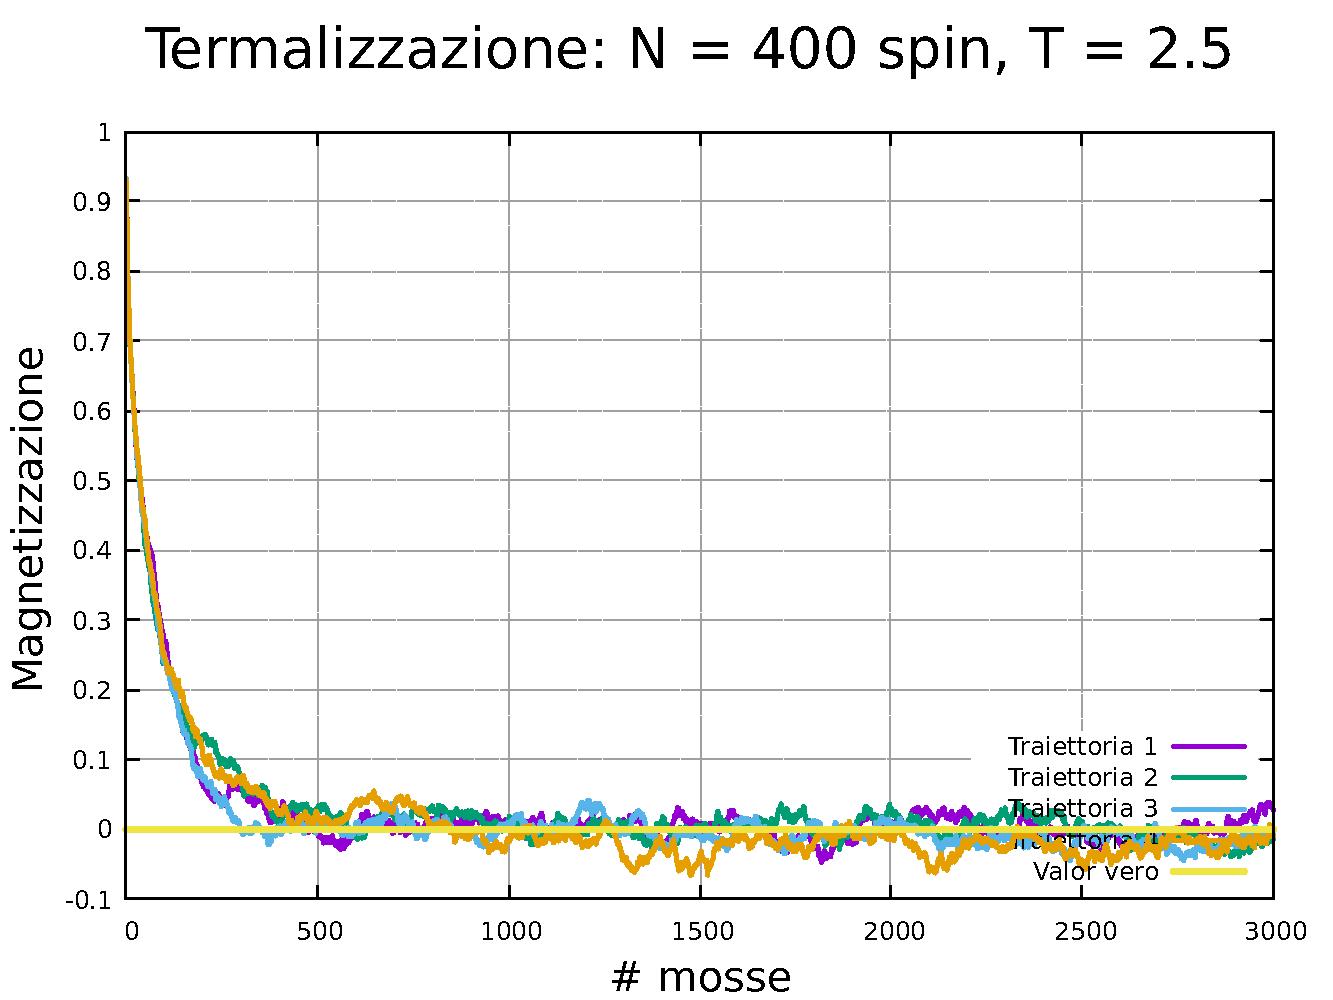
\includegraphics[page=1, width=\textwidth]{Immagini/simIsing2D/metro/term/term_400_2.5.pdf}
        \caption{$T\,=\,2.5$}
      \end{minipage}
    \vskip\baselineskip 
  
    \begin{minipage}{0.45\textwidth}  
      \centering
      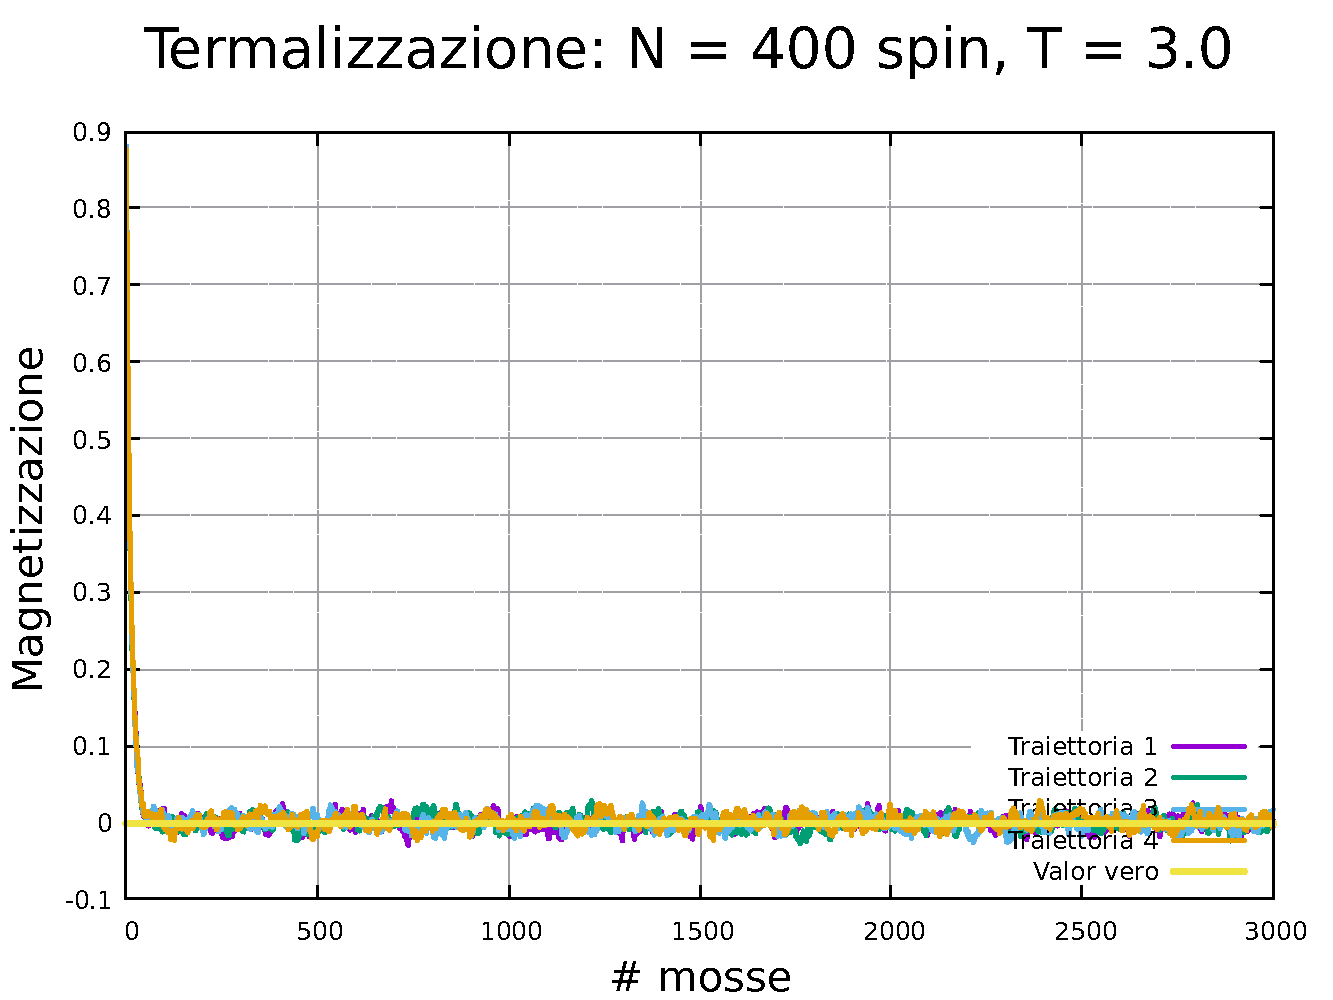
\includegraphics[page=1, width=\textwidth]{Immagini/simIsing2D/metro/term/term_400_3.0.pdf}
      \caption{$T\,=\,3.0$}
    \end{minipage}\hfill
    \begin{minipage}{0.45\textwidth}  
      \centering
      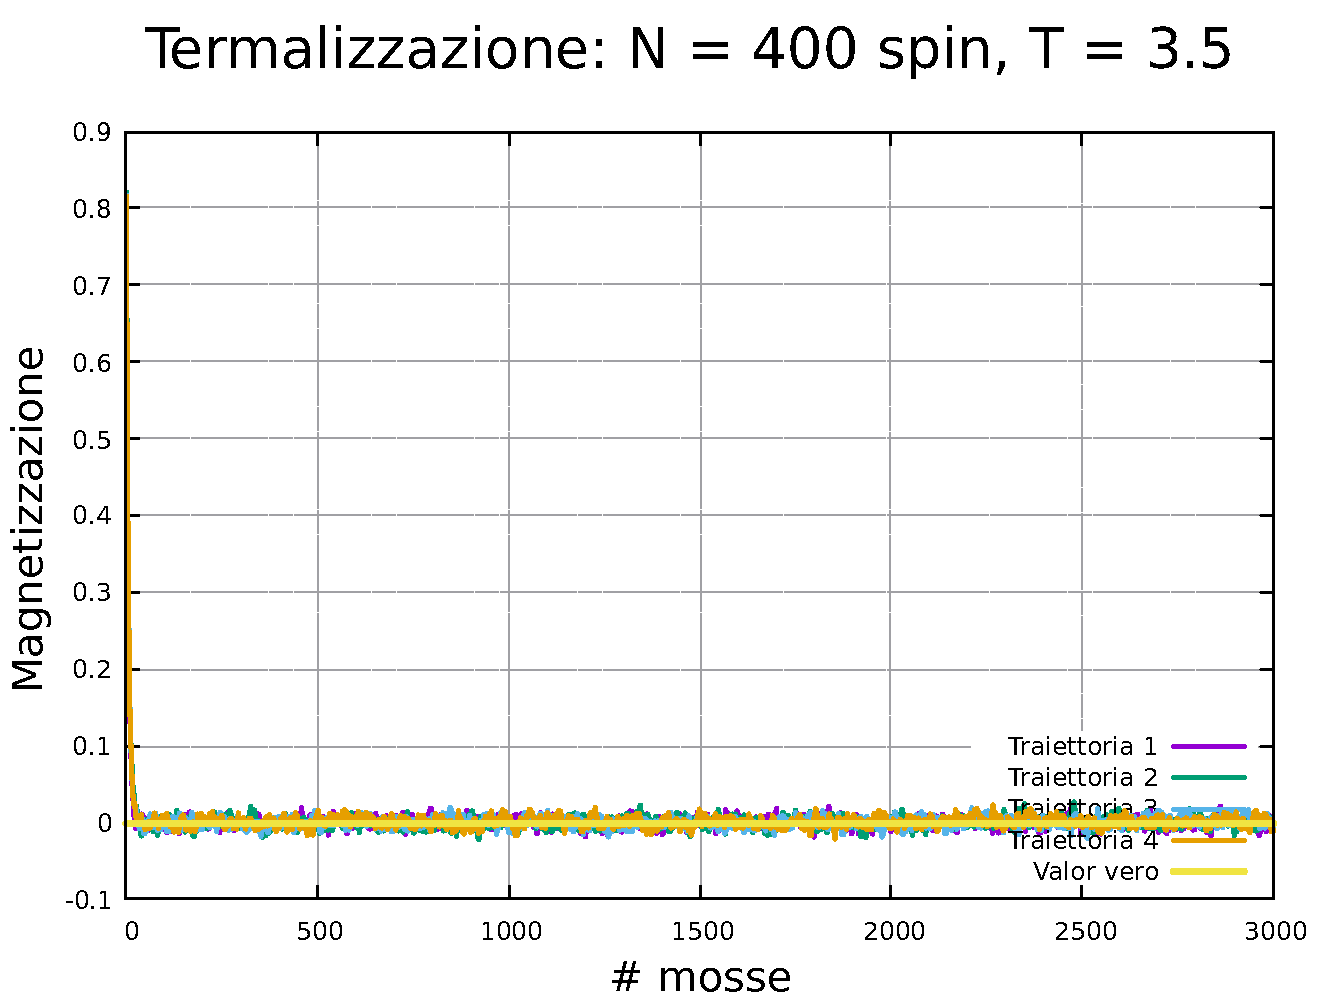
\includegraphics[page=1, width=\textwidth]{Immagini/simIsing2D/metro/term/term_400_3.5.pdf}
      \caption{$T\,=\,3.5$}
    \end{minipage}
    \caption{Studio della termalizzazione di un modello di Ising 2D costituito da $400 \times 400$ spin.}
\end{figure}

\vspace*{\fill}



\vspace*{\fill}

\begin{figure}[H]
    \centering
    \begin{minipage}{0.45\textwidth}  
      \centering
      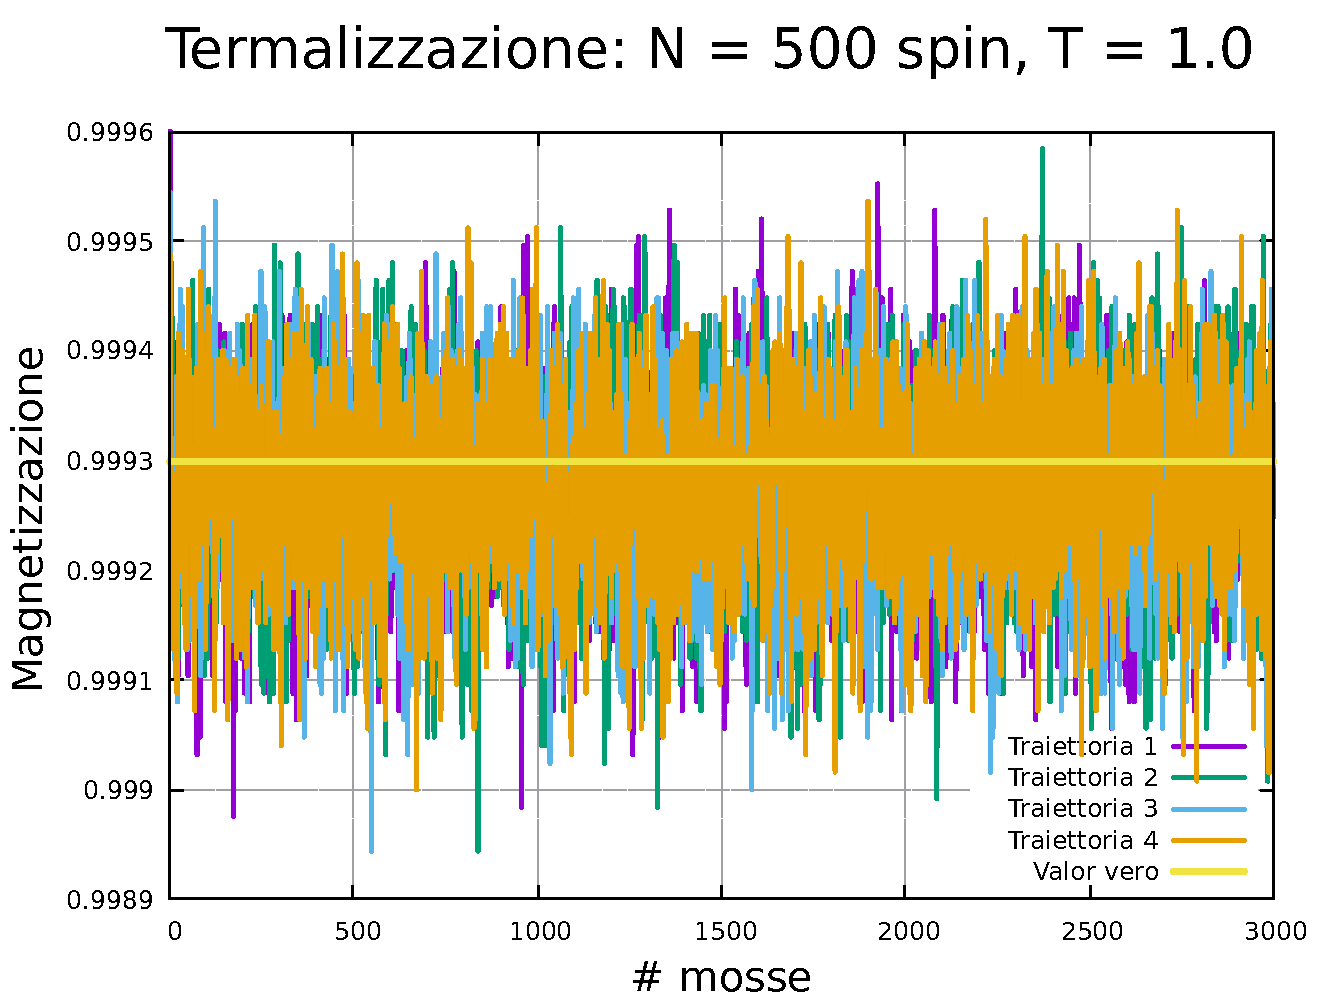
\includegraphics[page=1, width=\textwidth]{Immagini/simIsing2D/metro/term/term_500_1.0.pdf}
      \caption{$T\,=\,1.0$}
    \end{minipage}\hfill
    \begin{minipage}{0.45\textwidth}  
      \centering
      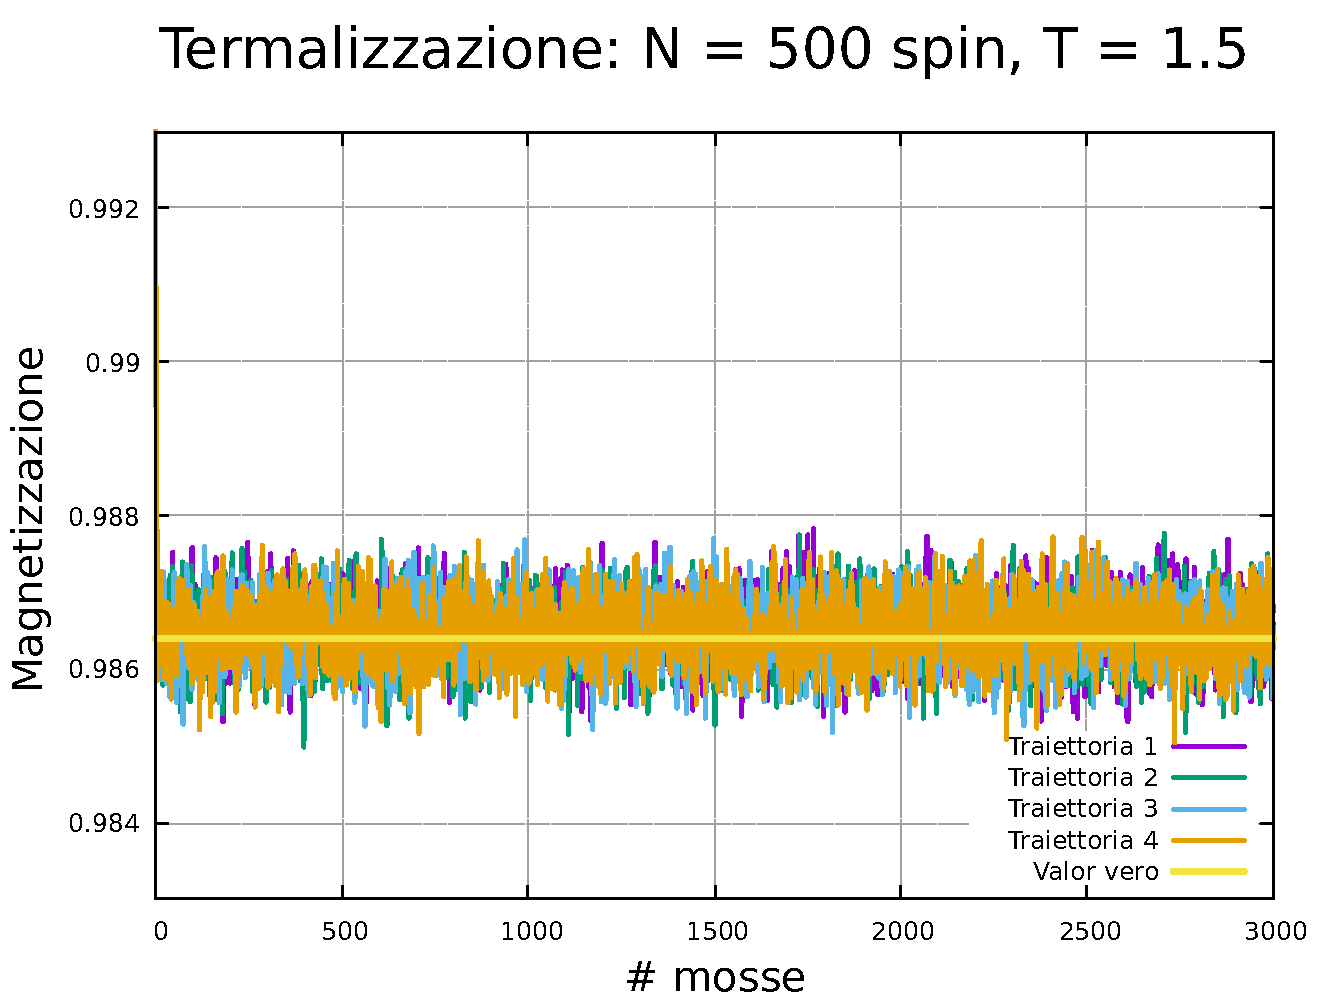
\includegraphics[page=1, width=\textwidth]{Immagini/simIsing2D/metro/term/term_500_1.5.pdf}
      \caption{$T\,=\,1.5$}
    \end{minipage}
    \vskip\baselineskip 

    \begin{minipage}{0.45\textwidth}  
        \centering
        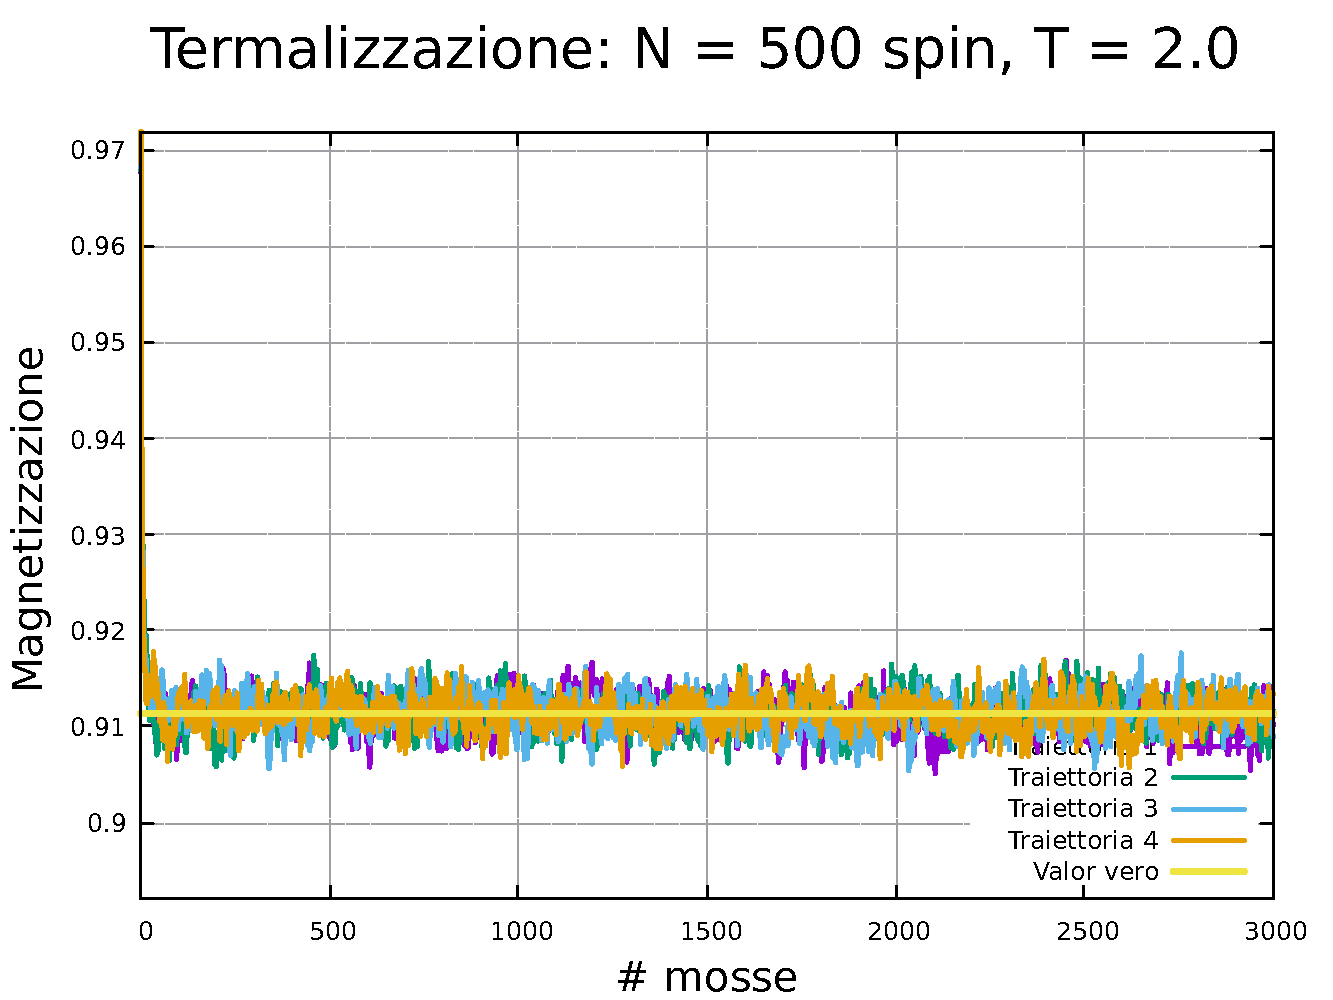
\includegraphics[page=1, width=\textwidth]{Immagini/simIsing2D/metro/term/term_500_2.0.pdf}
        \caption{$T\,=\,2.0$}
      \end{minipage}\hfill
      \begin{minipage}{0.45\textwidth}  
        \centering
        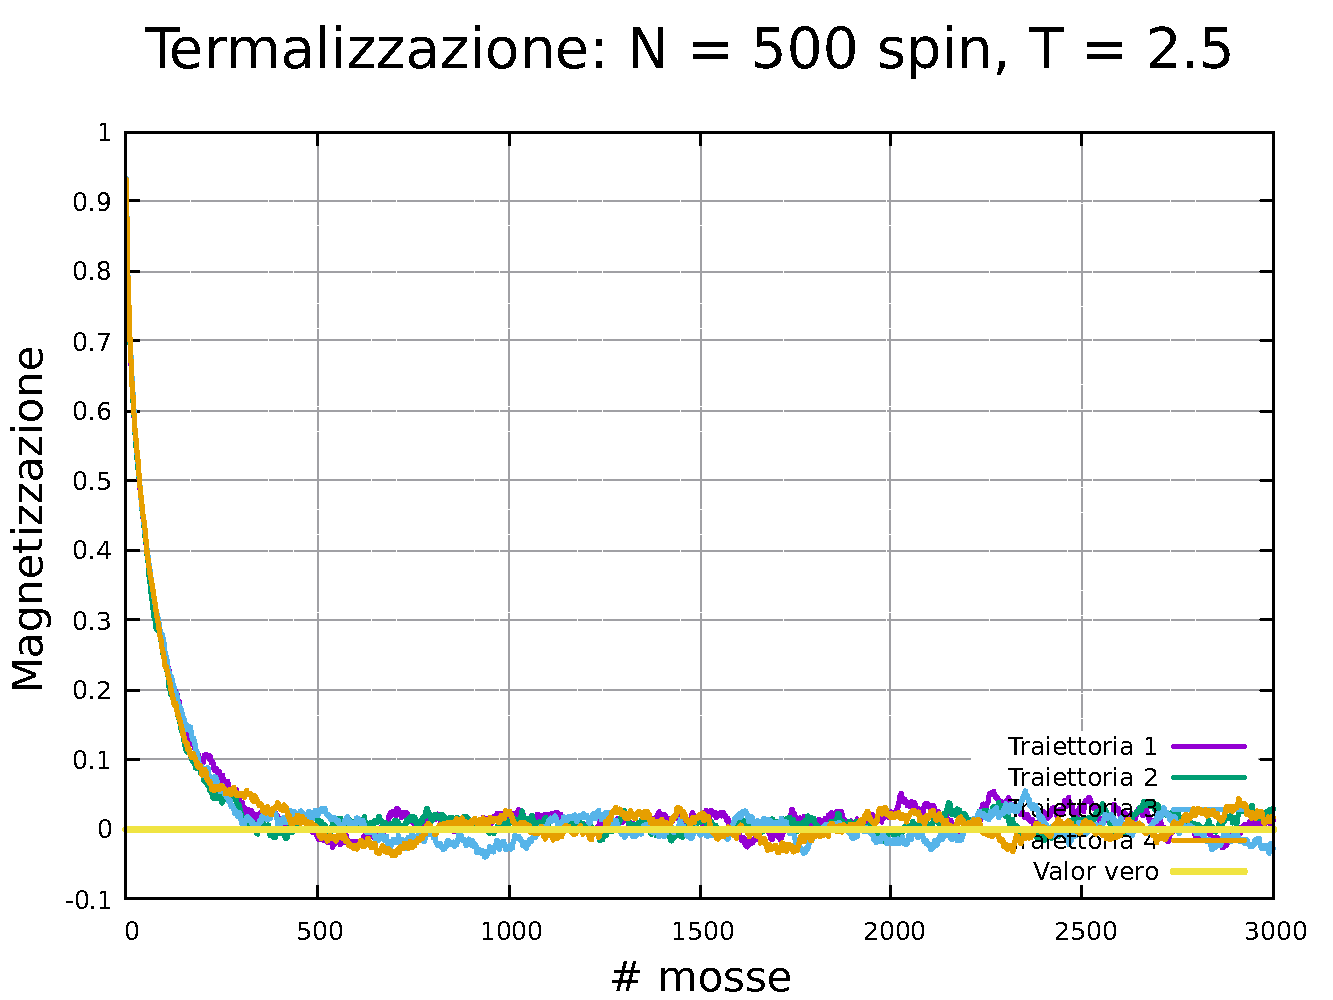
\includegraphics[page=1, width=\textwidth]{Immagini/simIsing2D/metro/term/term_500_2.5.pdf}
        \caption{$T\,=\,2.5$}
      \end{minipage}
    \vskip\baselineskip 
  
    \begin{minipage}{0.45\textwidth}  
      \centering
      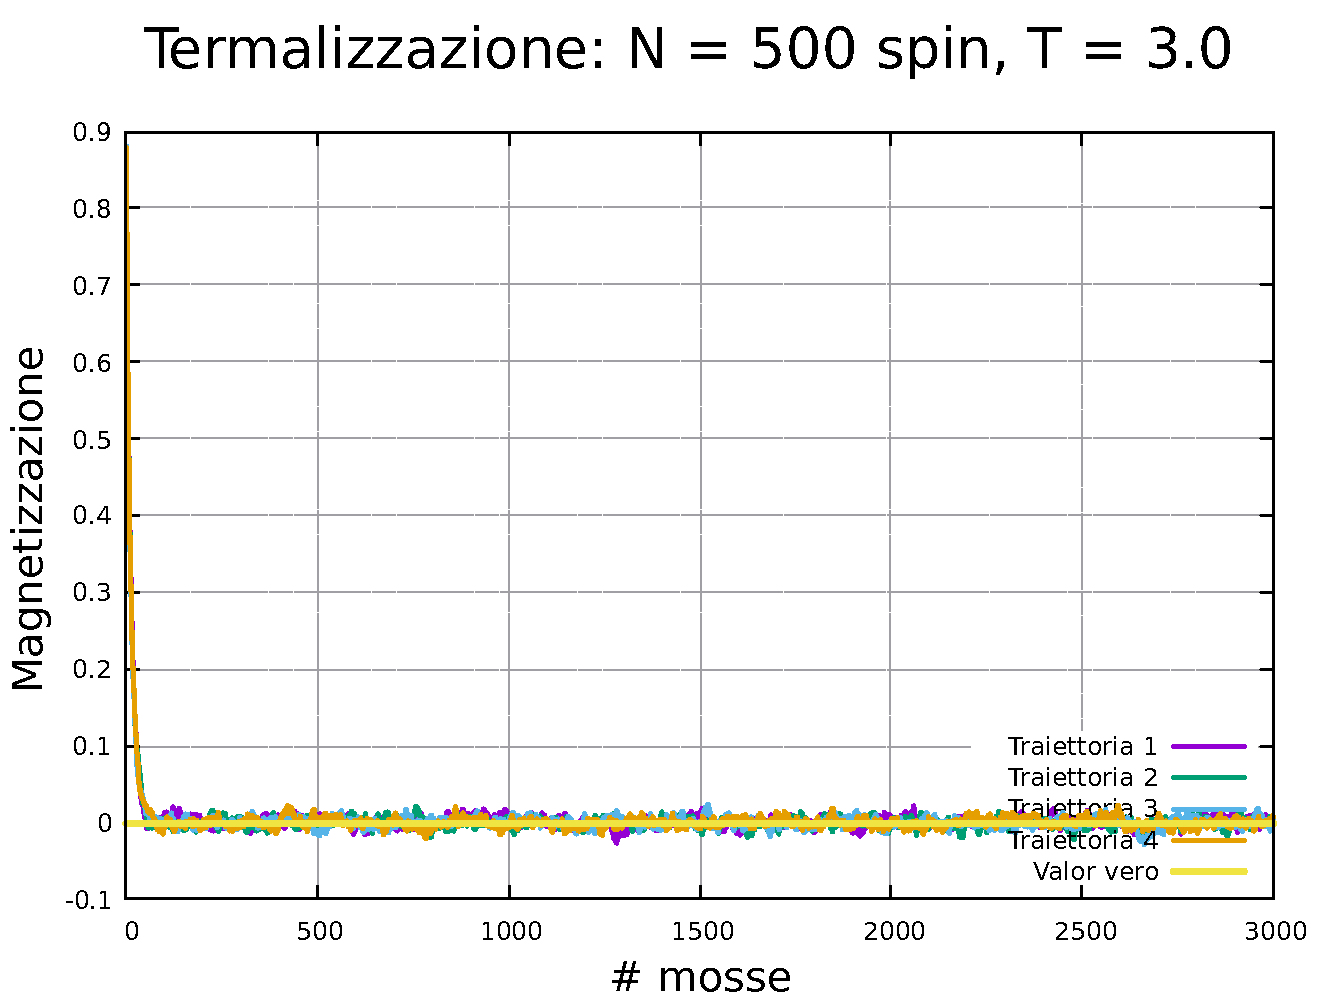
\includegraphics[page=1, width=\textwidth]{Immagini/simIsing2D/metro/term/term_500_3.0.pdf}
      \caption{$T\,=\,3.0$}
    \end{minipage}\hfill
    \begin{minipage}{0.45\textwidth}  
      \centering
      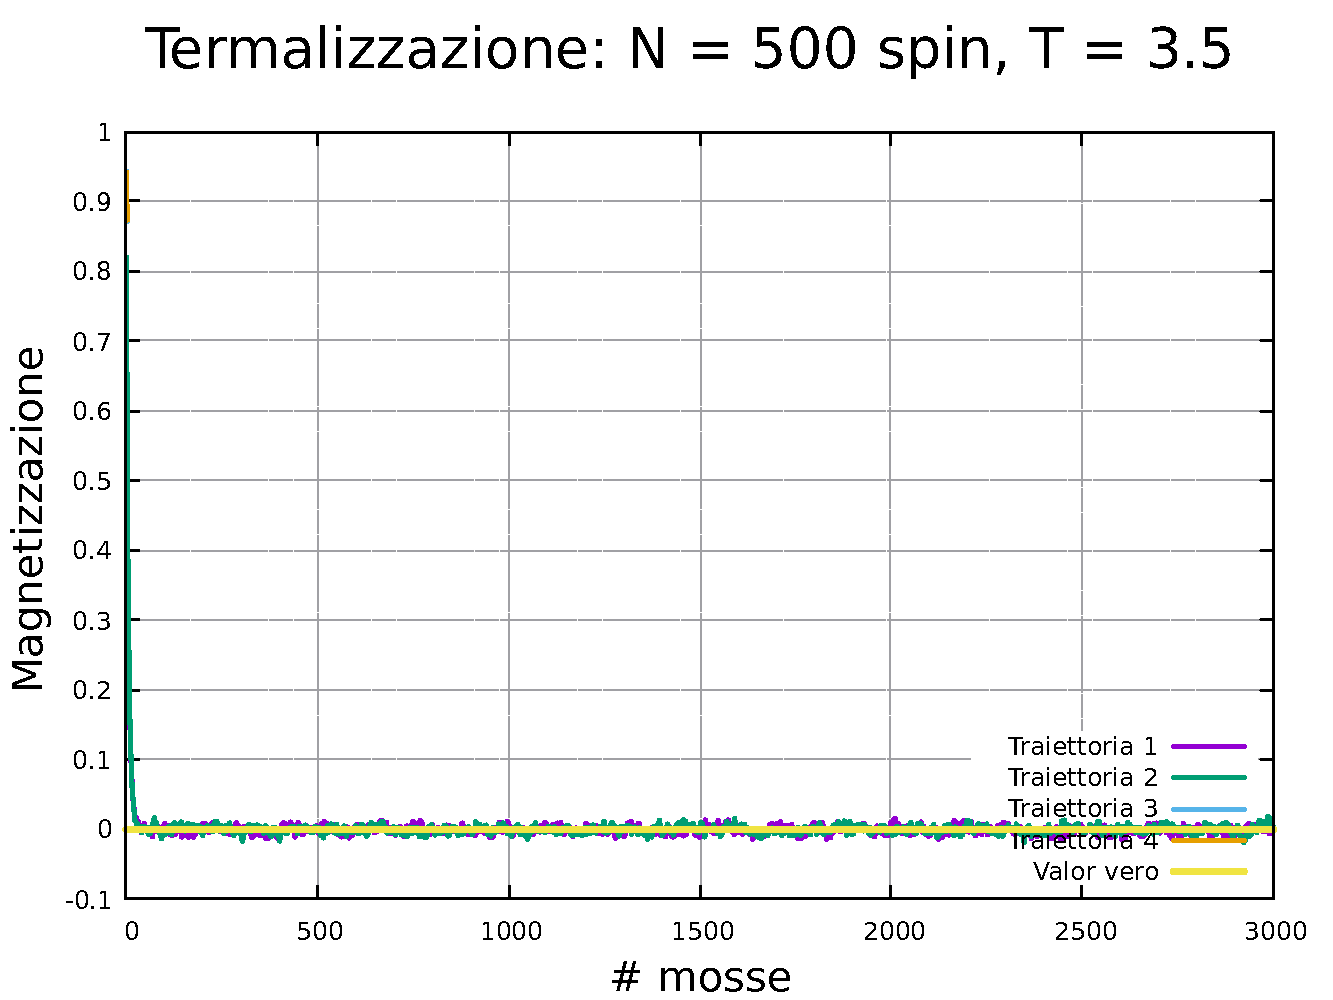
\includegraphics[page=1, width=\textwidth]{Immagini/simIsing2D/metro/term/term_500_3.5.pdf}
      \caption{$T\,=\,3.5$}
    \end{minipage}
    \caption{Studio della termalizzazione di un modello di Ising 2D costituito da $500 \times 500$ spin.}
\end{figure}

\vspace*{\fill}




















\subsection{Autocorrelazione}

\vspace*{\fill}
\begin{figure}[H]
    \centering
    \begin{minipage}{0.45\textwidth}  
      \centering
      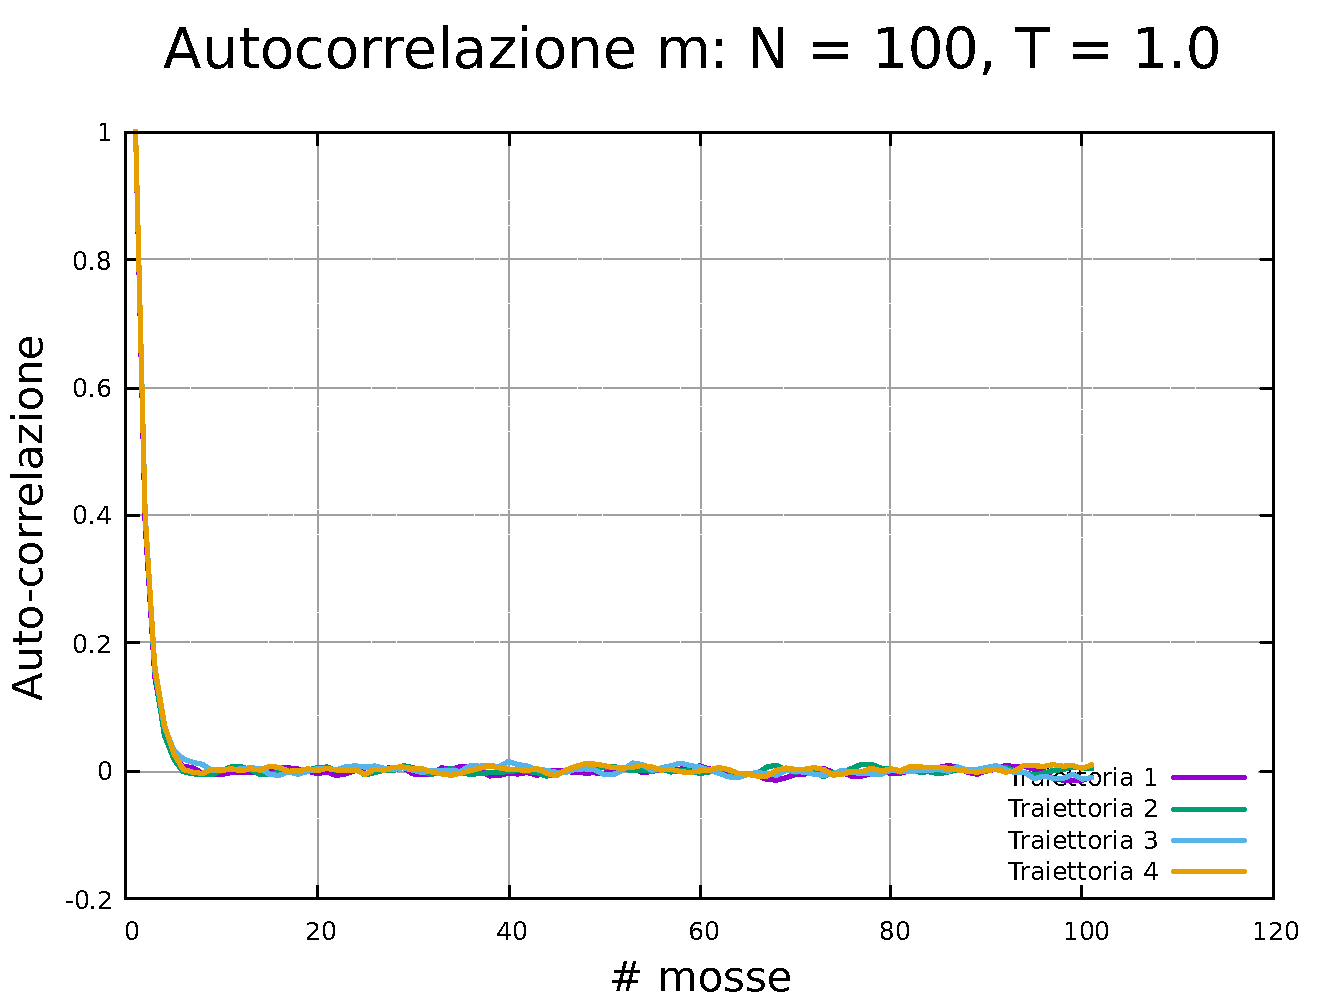
\includegraphics[page=1, width=\textwidth]{Immagini/simIsing2D/metro/tcorr/auto_100_1.0.pdf}
      \caption{$T\,=\,1.0$}
    \end{minipage}\hfill
    \begin{minipage}{0.45\textwidth}  
      \centering
      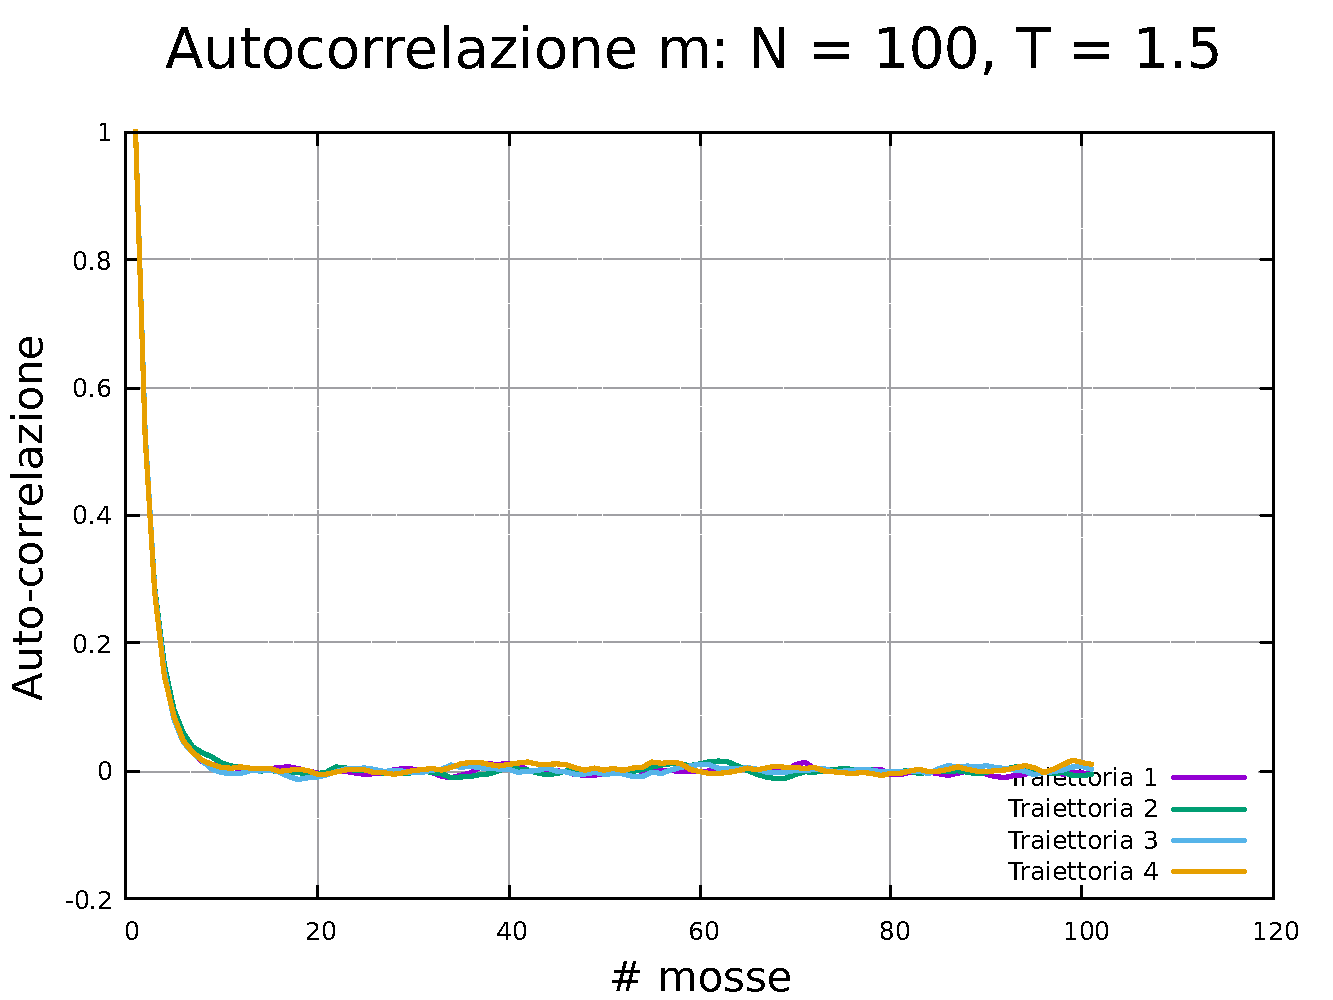
\includegraphics[page=1, width=\textwidth]{Immagini/simIsing2D/metro/tcorr/auto_100_1.5.pdf}
      \caption{$T\,=\,1.5$}
    \end{minipage}
    \vskip\baselineskip 

    \begin{minipage}{0.45\textwidth}  
        \centering
        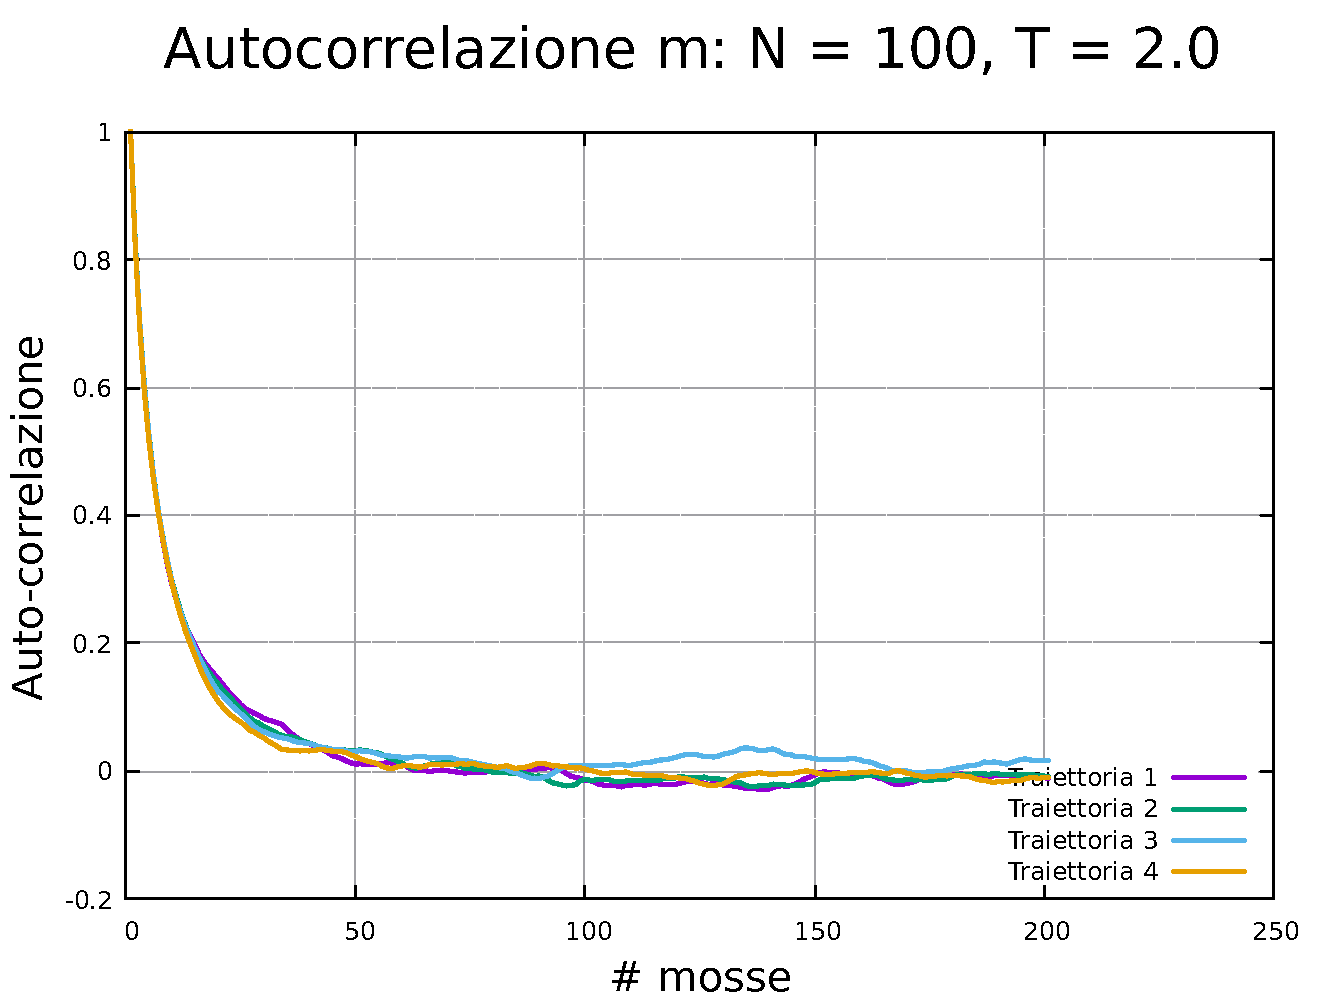
\includegraphics[page=1, width=\textwidth]{Immagini/simIsing2D/metro/tcorr/auto_100_2.0.pdf}
        \caption{$T\,=\,2.0$}
      \end{minipage}\hfill
      \begin{minipage}{0.45\textwidth}  
        \centering
        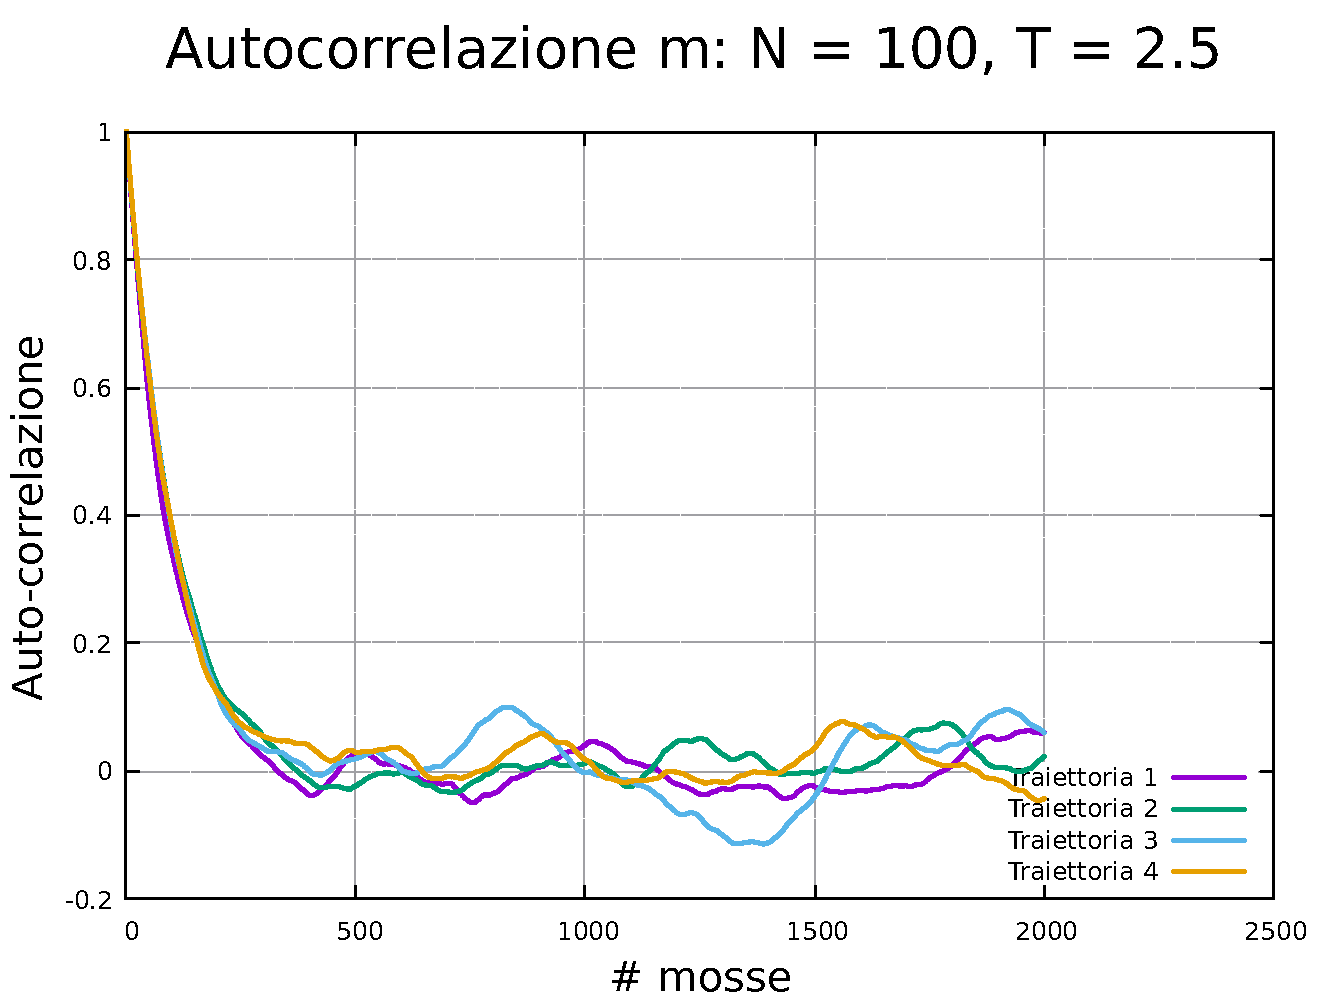
\includegraphics[page=1, width=\textwidth]{Immagini/simIsing2D/metro/tcorr/auto_100_2.5.pdf}
        \caption{$T\,=\,2.5$}
      \end{minipage}
    \vskip\baselineskip 
  
    \begin{minipage}{0.45\textwidth}  
      \centering
      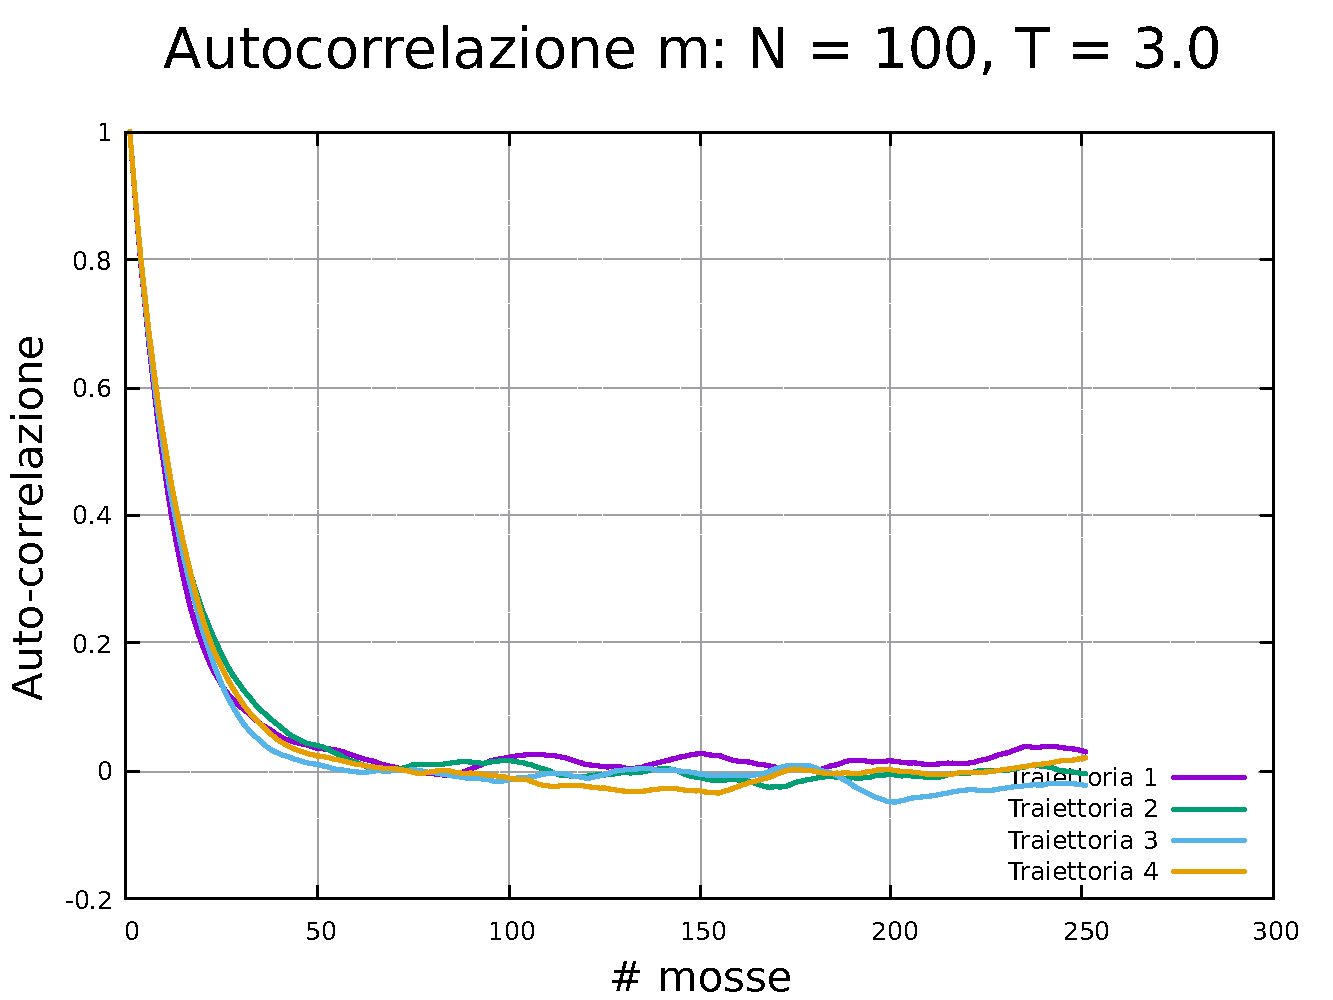
\includegraphics[page=1, width=\textwidth]{Immagini/simIsing2D/metro/tcorr/auto_100_3.0.pdf}
      \caption{$T\,=\,3.0$}
    \end{minipage}\hfill
    \begin{minipage}{0.45\textwidth}  
      \centering
      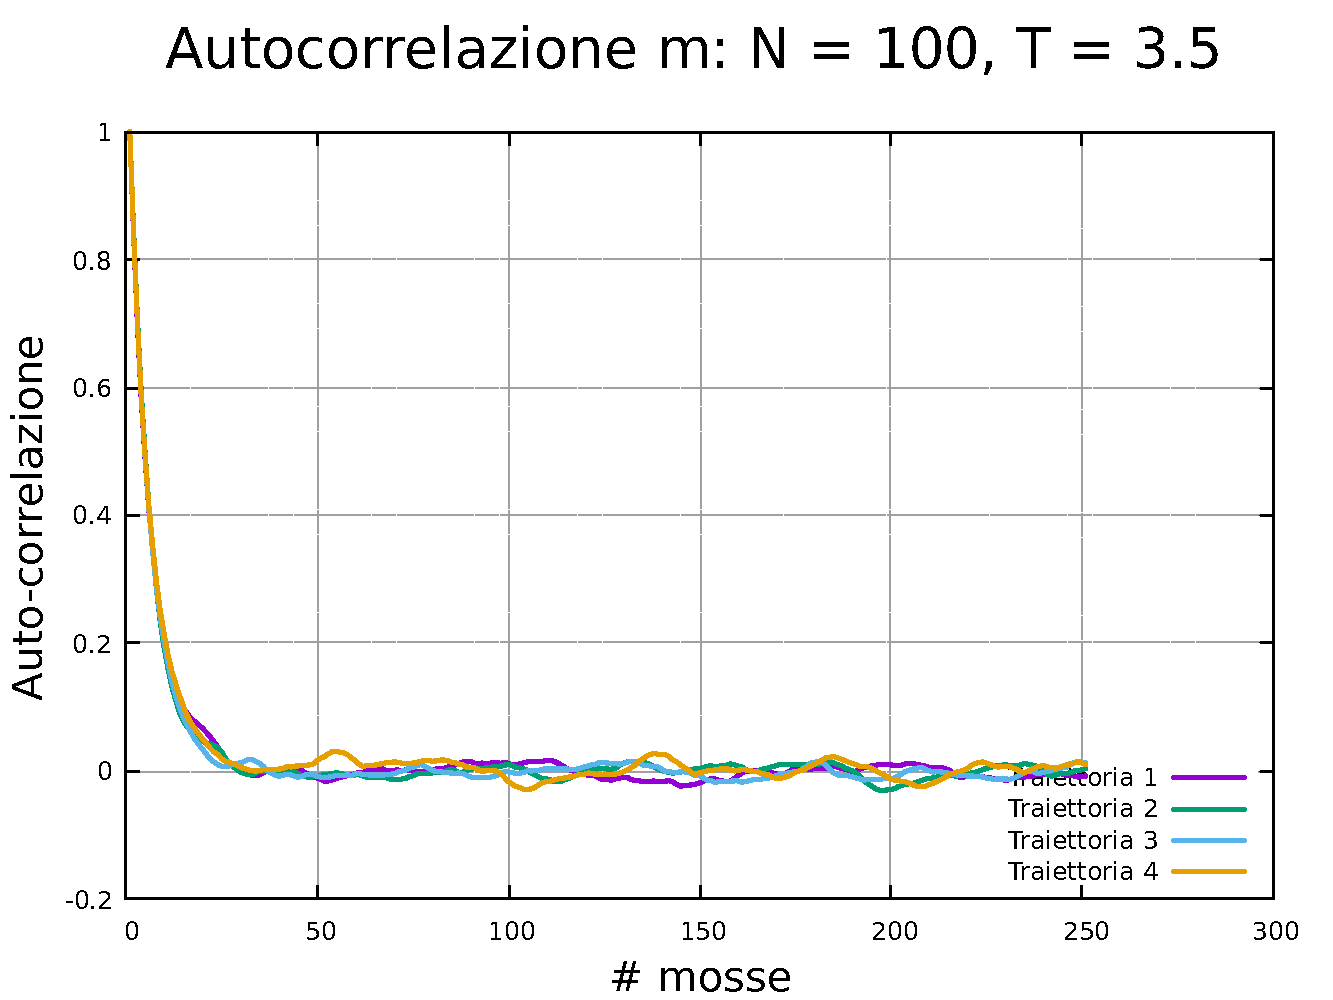
\includegraphics[page=1, width=\textwidth]{Immagini/simIsing2D/metro/tcorr/auto_100_3.5.pdf}
      \caption{$T\,=\,3.5$}
    \end{minipage}
    \caption{Studio dell'autocorrelazione di un modello di Ising 2D costituito da $100 \times 100$ spin.}
\end{figure}

\vspace*{\fill}



\vspace*{\fill}

\begin{figure}[H]
    \centering
    \begin{minipage}{0.45\textwidth}  
      \centering
      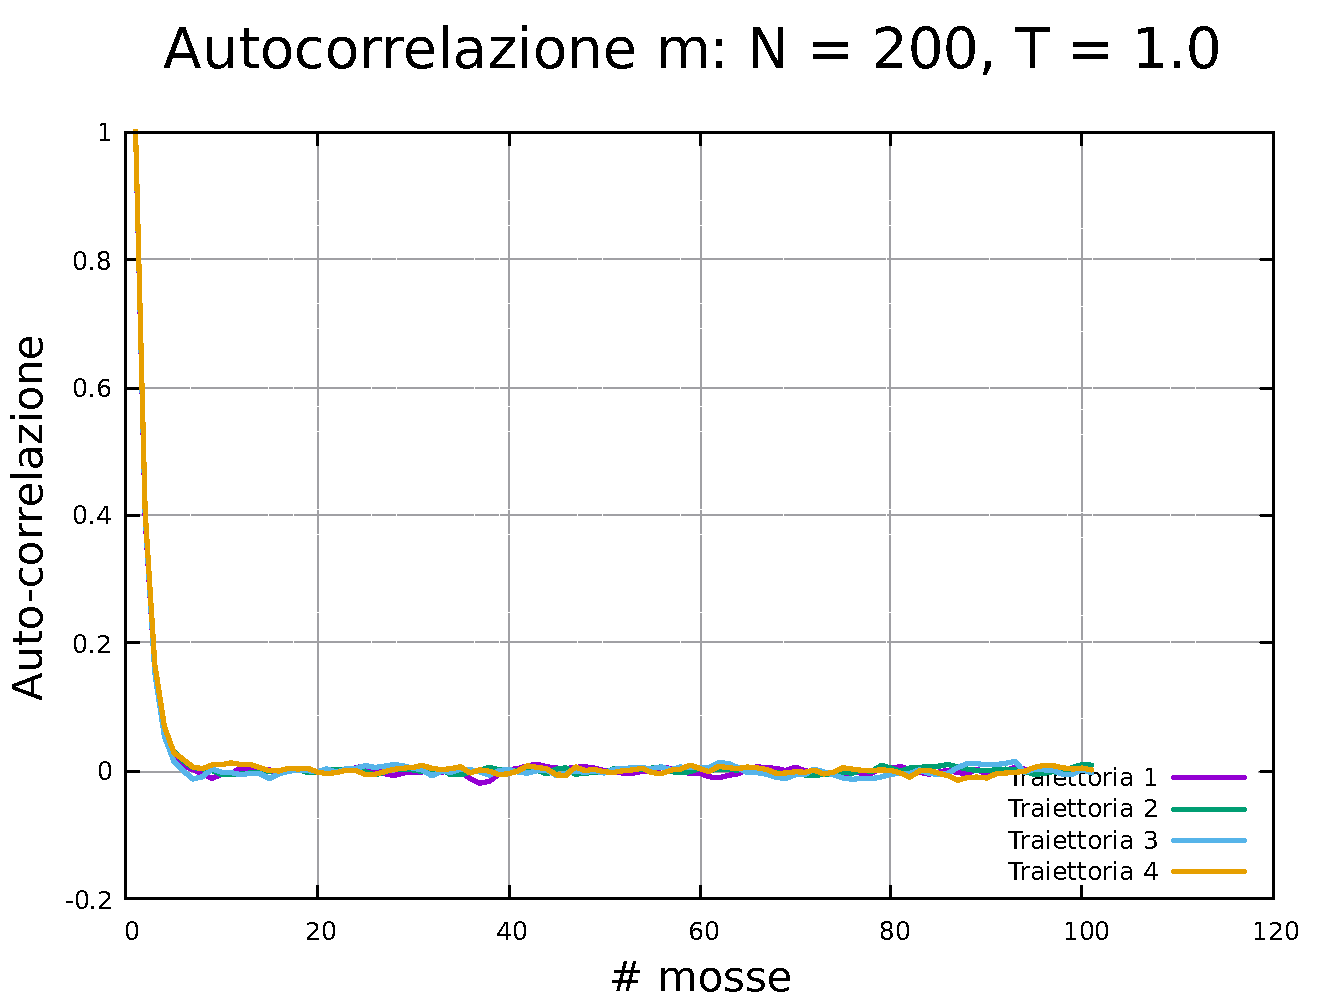
\includegraphics[page=1, width=\textwidth]{Immagini/simIsing2D/metro/tcorr/auto_200_1.0.pdf}
      \caption{$T\,=\,1.0$}
    \end{minipage}\hfill
    \begin{minipage}{0.45\textwidth}  
      \centering
      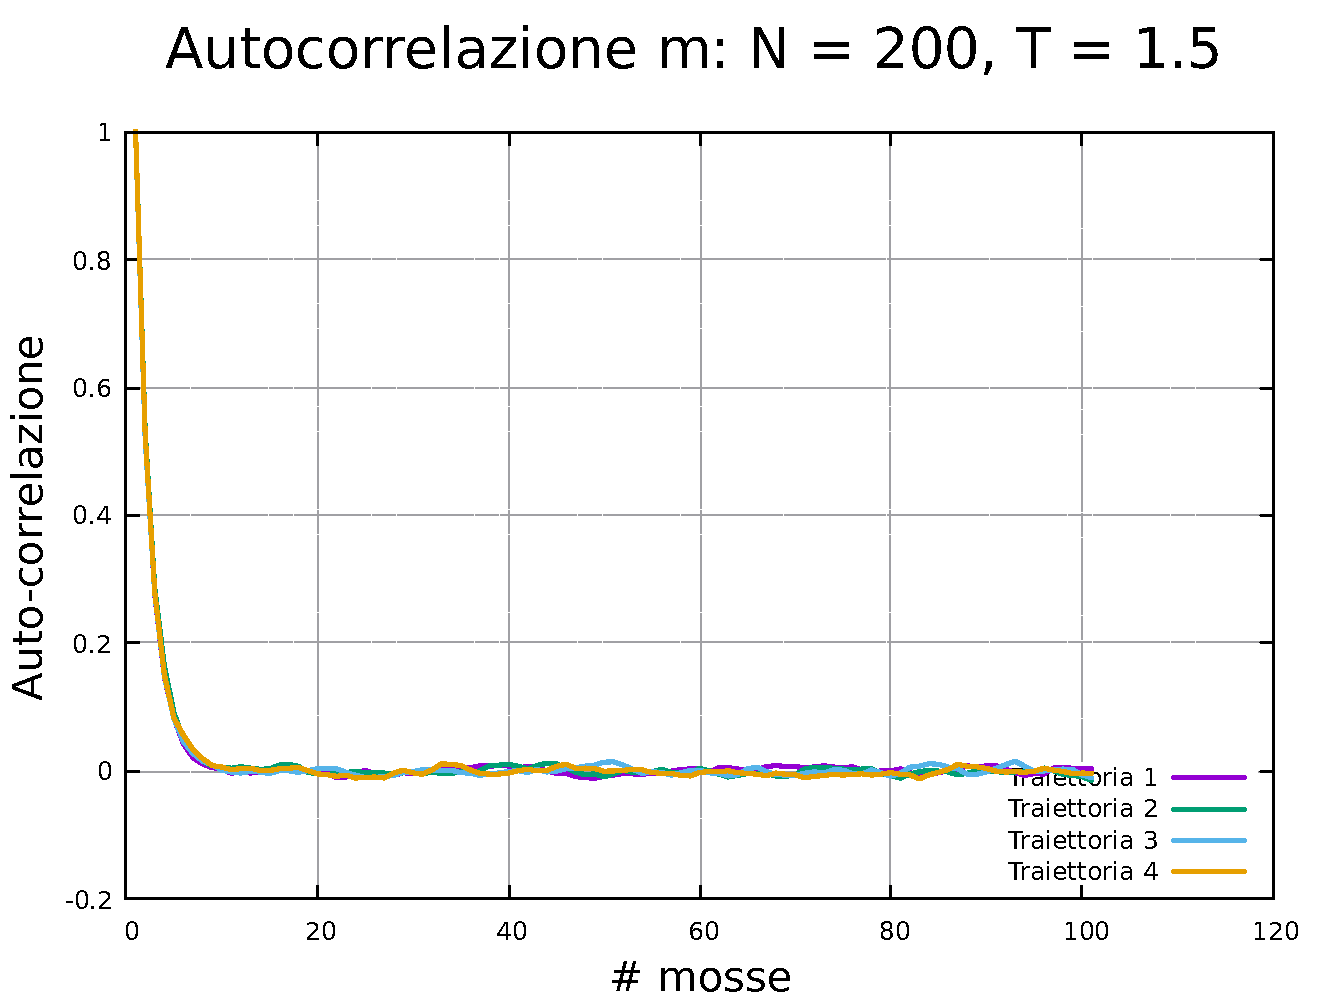
\includegraphics[page=1, width=\textwidth]{Immagini/simIsing2D/metro/tcorr/auto_200_1.5.pdf}
      \caption{$T\,=\,1.5$}
    \end{minipage}
    \vskip\baselineskip 
  
    \begin{minipage}{0.45\textwidth}  
      \centering
      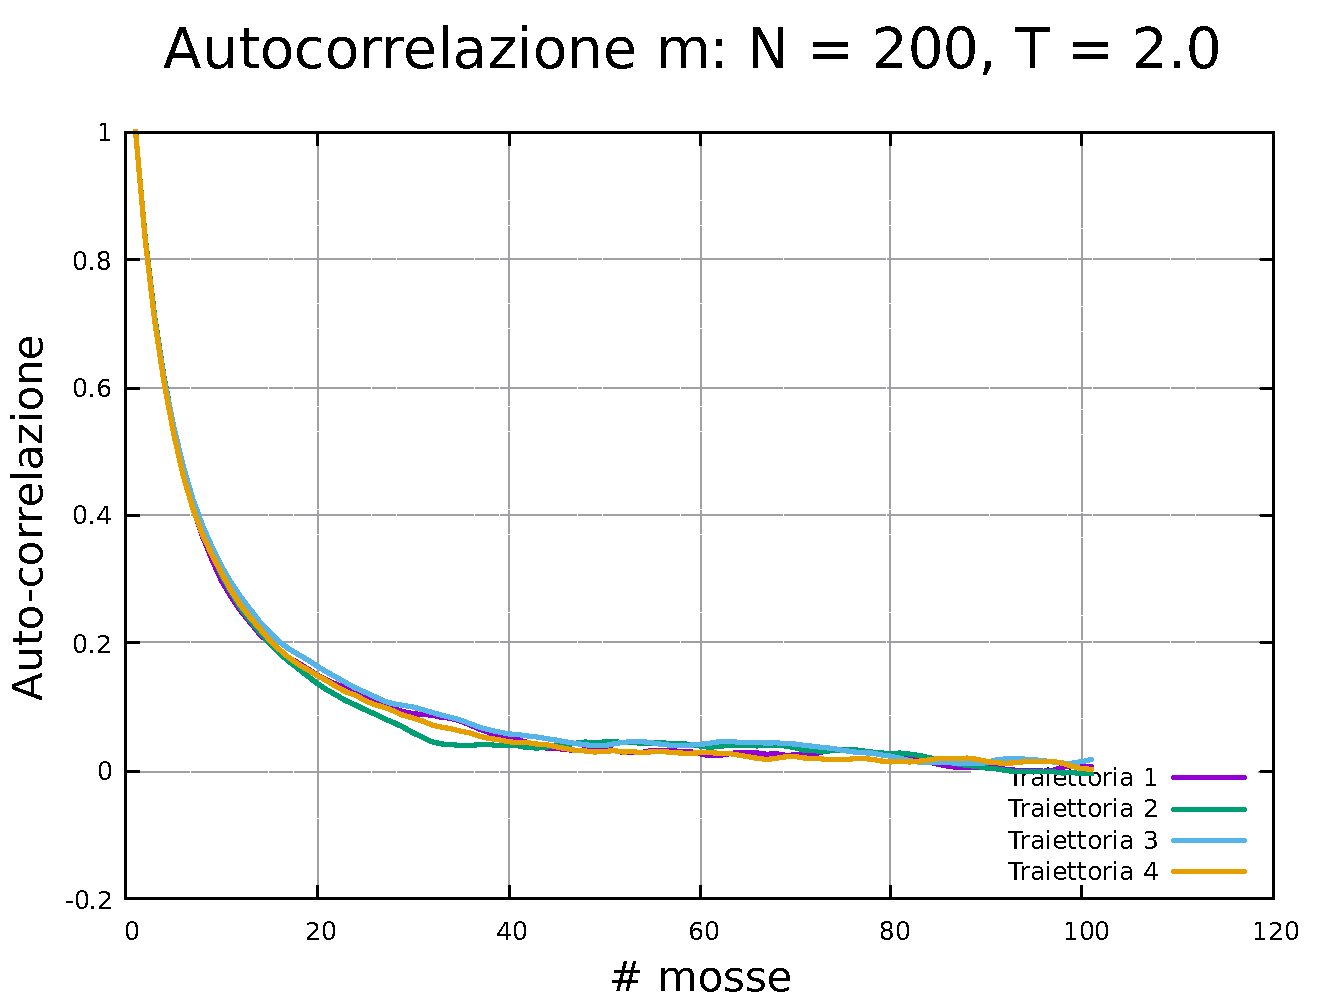
\includegraphics[page=1, width=\textwidth]{Immagini/simIsing2D/metro/tcorr/auto_200_2.0.pdf}
      \caption{$T\,=\,2.0$}
    \end{minipage}\hfill
    \begin{minipage}{0.45\textwidth}  
      \centering
      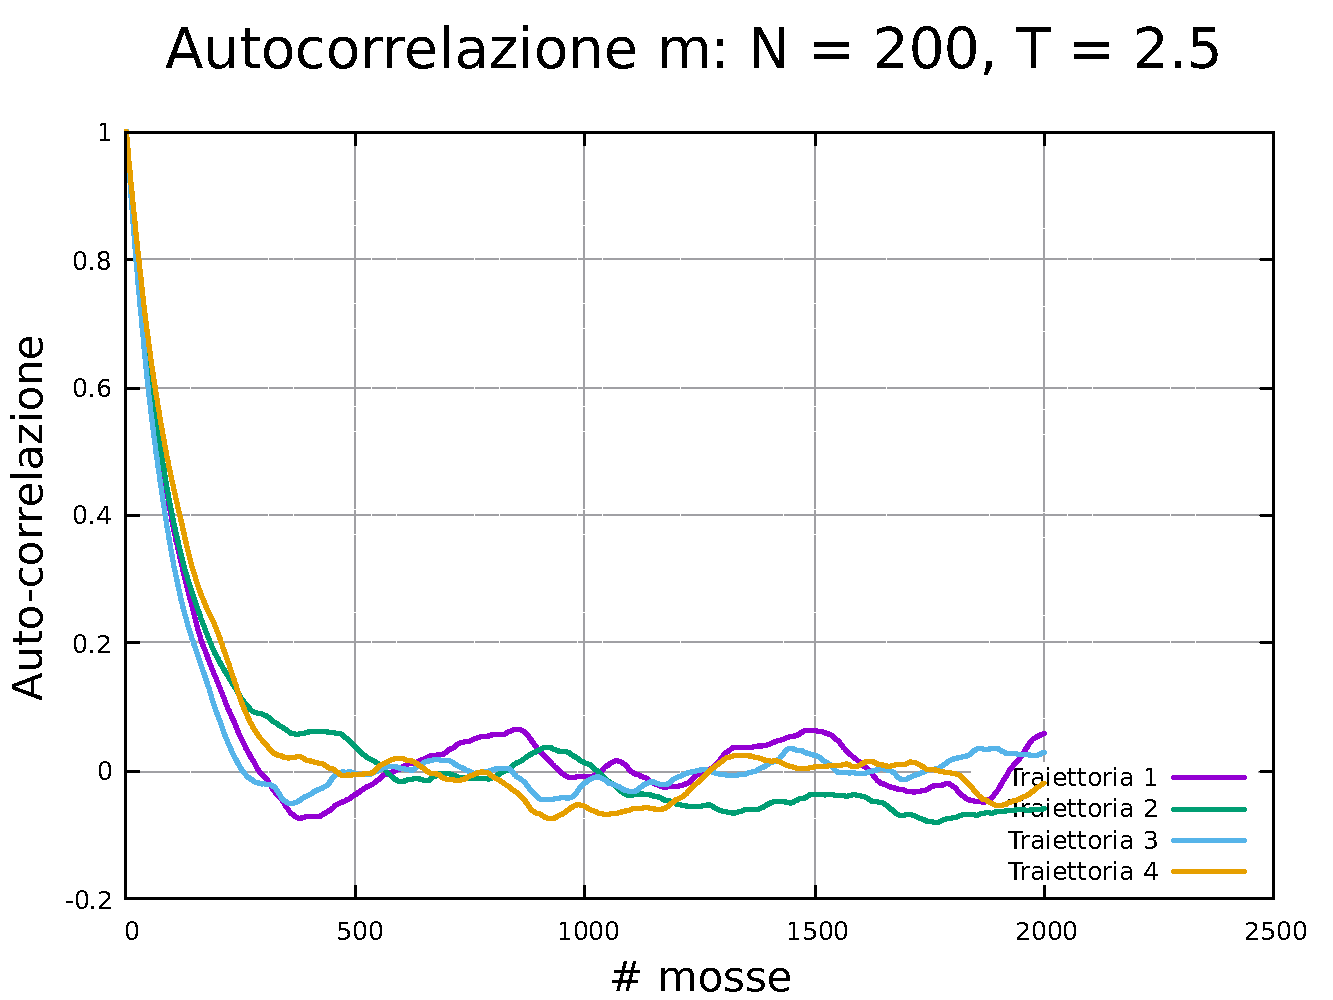
\includegraphics[page=1, width=\textwidth]{Immagini/simIsing2D/metro/tcorr/auto_200_2.5.pdf}
      \caption{$T\,=\,2.5$}
    \end{minipage}
    \vskip\baselineskip 

    \begin{minipage}{0.45\textwidth}  
        \centering
        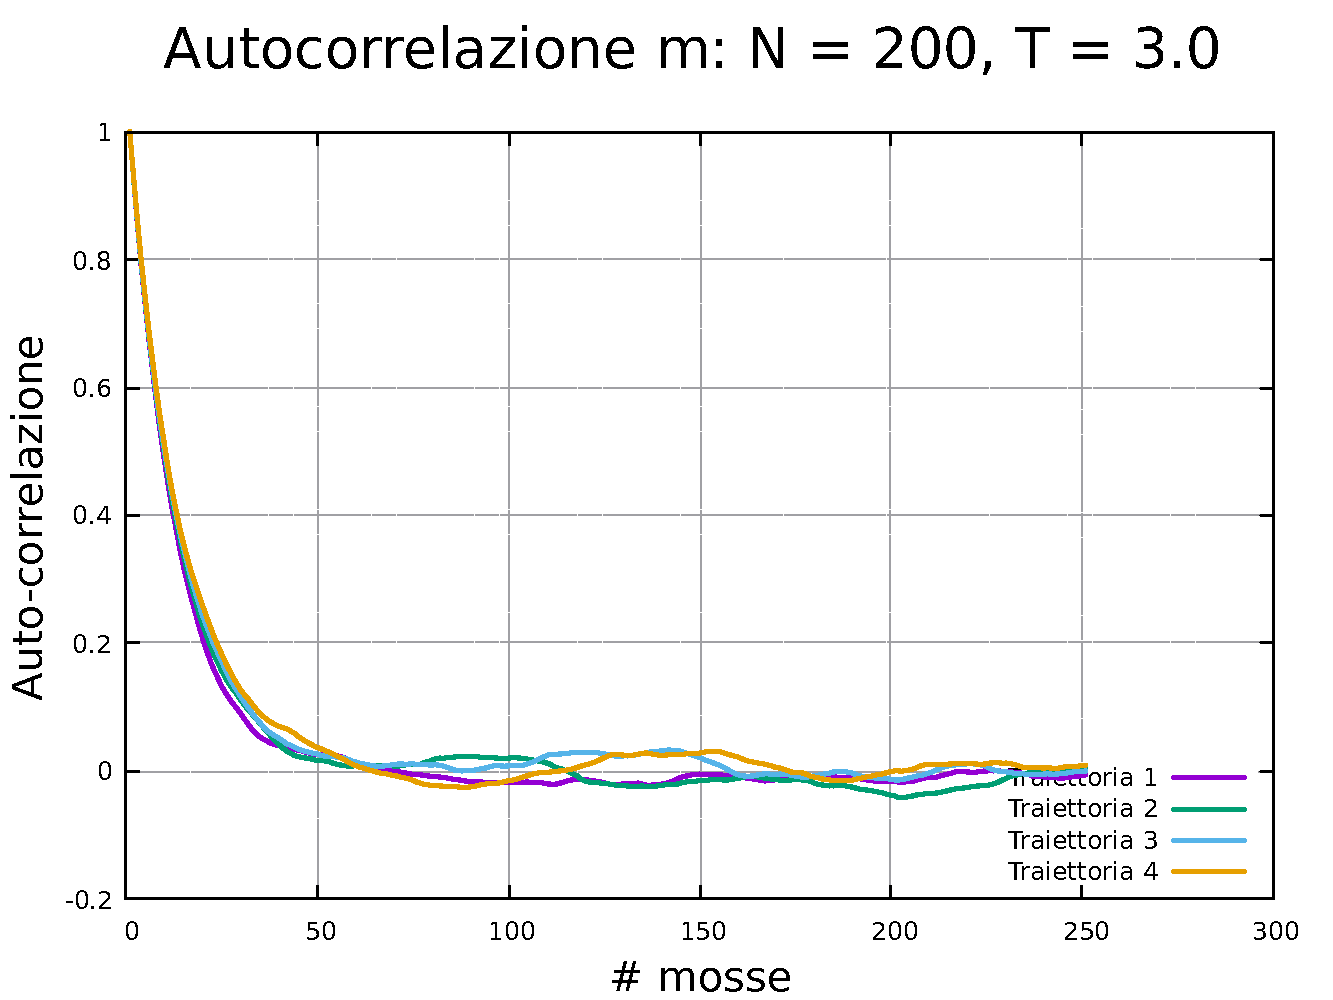
\includegraphics[page=1, width=\textwidth]{Immagini/simIsing2D/metro/tcorr/auto_200_3.0.pdf}
        \caption{$T\,=\,3.0$}
      \end{minipage}\hfill
      \begin{minipage}{0.45\textwidth}  
        \centering
        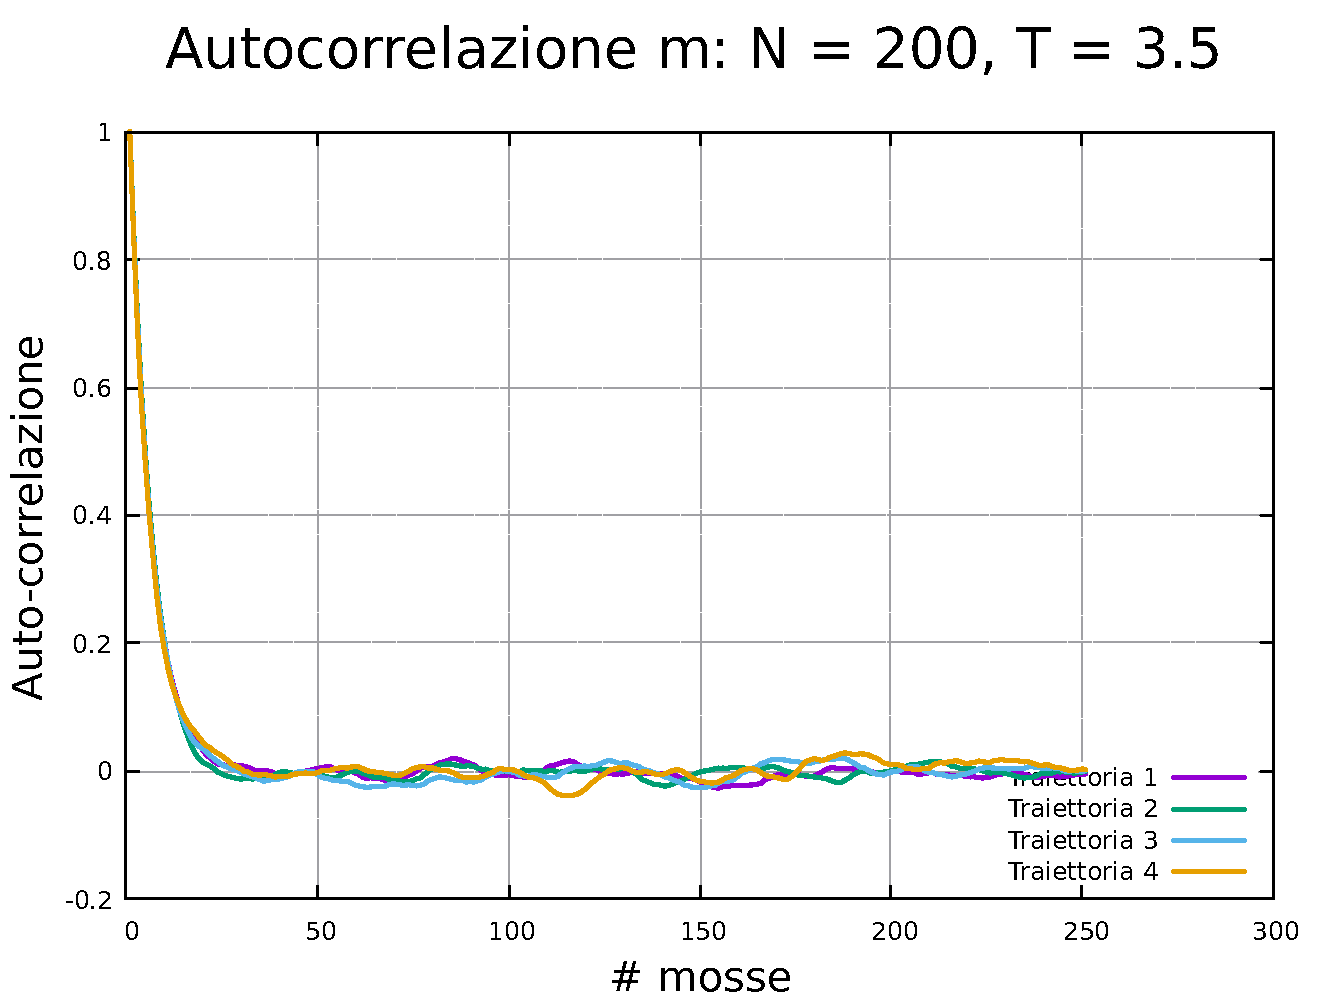
\includegraphics[page=1, width=\textwidth]{Immagini/simIsing2D/metro/tcorr/auto_200_3.5.pdf}
        \caption{$T\,=\,3.5$}
    \end{minipage}

    \caption{Studio dell'autocorrelazione di un modello di Ising 2D costituito da $200 \times 200$ spin.}
\end{figure}

\vspace*{\fill}



\vspace*{\fill}

\begin{figure}[H]
    \centering
    \begin{minipage}{0.45\textwidth}  
      \centering
      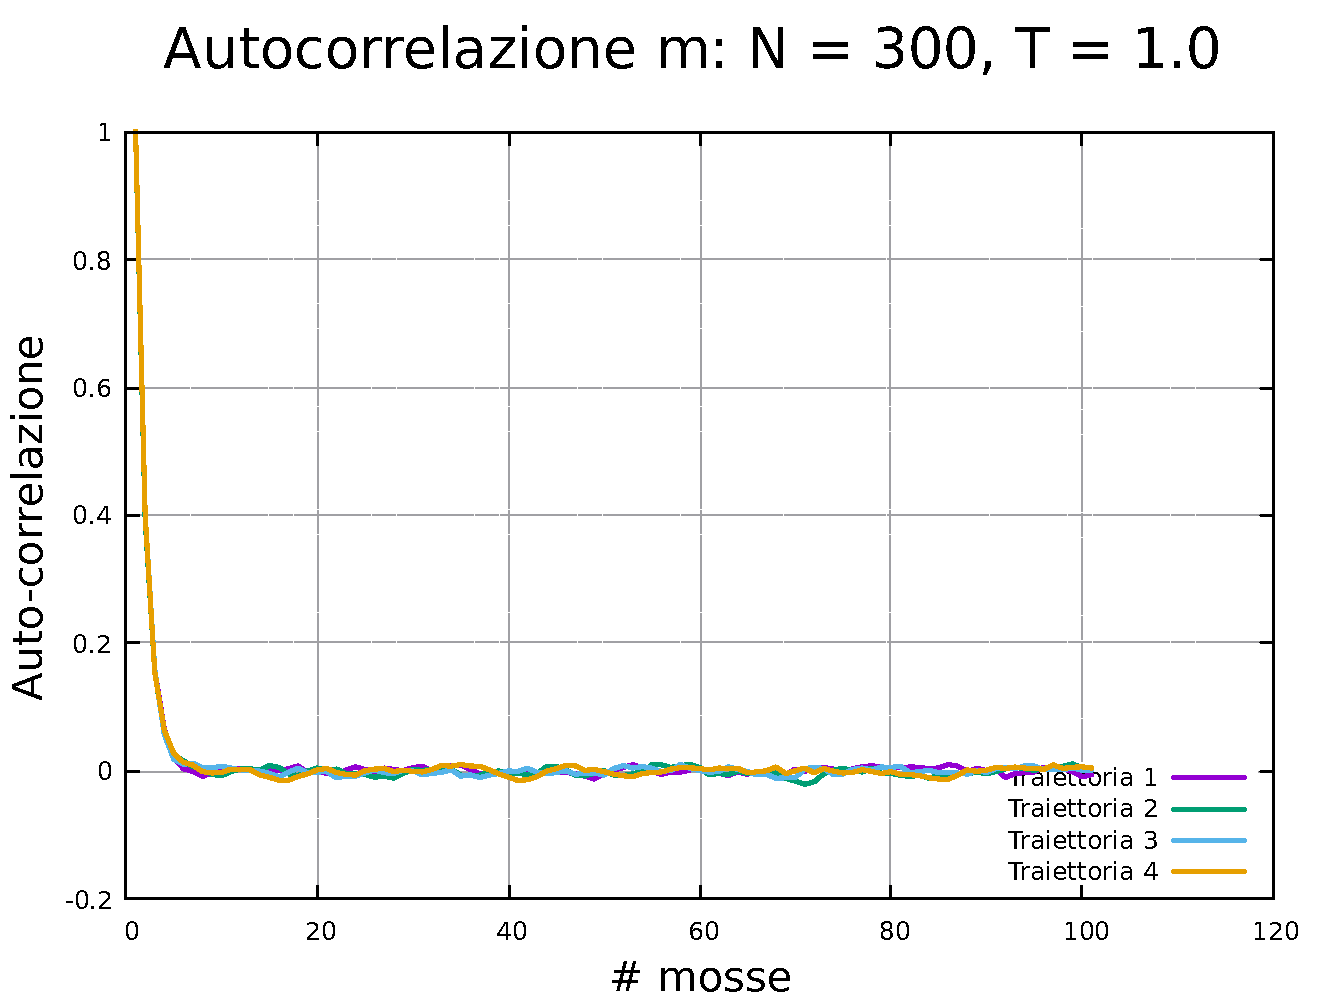
\includegraphics[page=1, width=\textwidth]{Immagini/simIsing2D/metro/tcorr/auto_300_1.0.pdf}
      \caption{$T\,=\,1.0$}
    \end{minipage}\hfill
    \begin{minipage}{0.45\textwidth}  
      \centering
      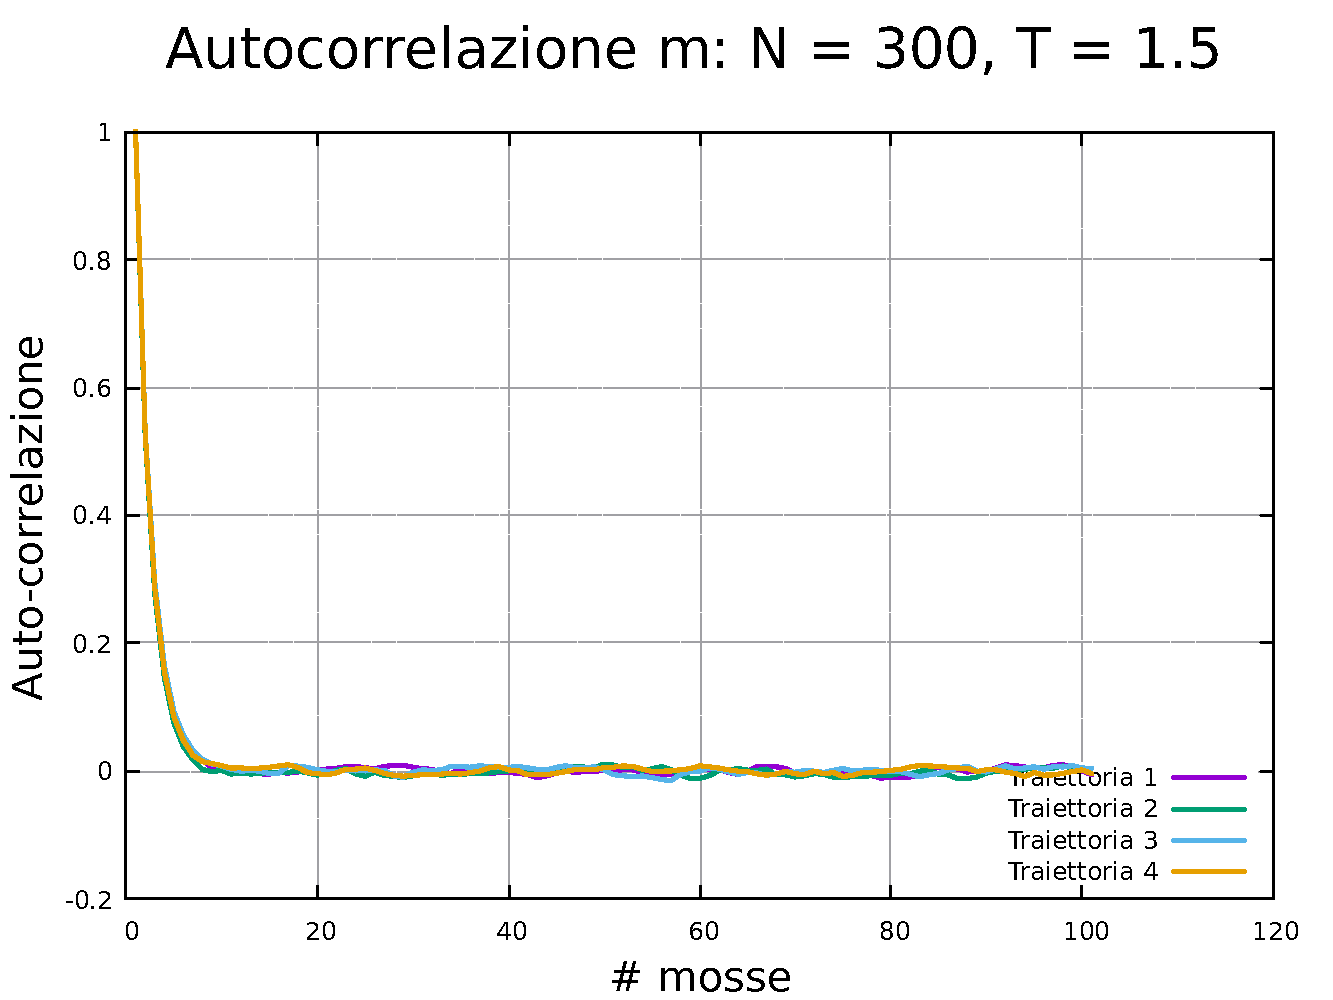
\includegraphics[page=1, width=\textwidth]{Immagini/simIsing2D/metro/tcorr/auto_300_1.5.pdf}
      \caption{$T\,=\,1.5$}
    \end{minipage}
    \vskip\baselineskip 

    \begin{minipage}{0.45\textwidth}  
        \centering
        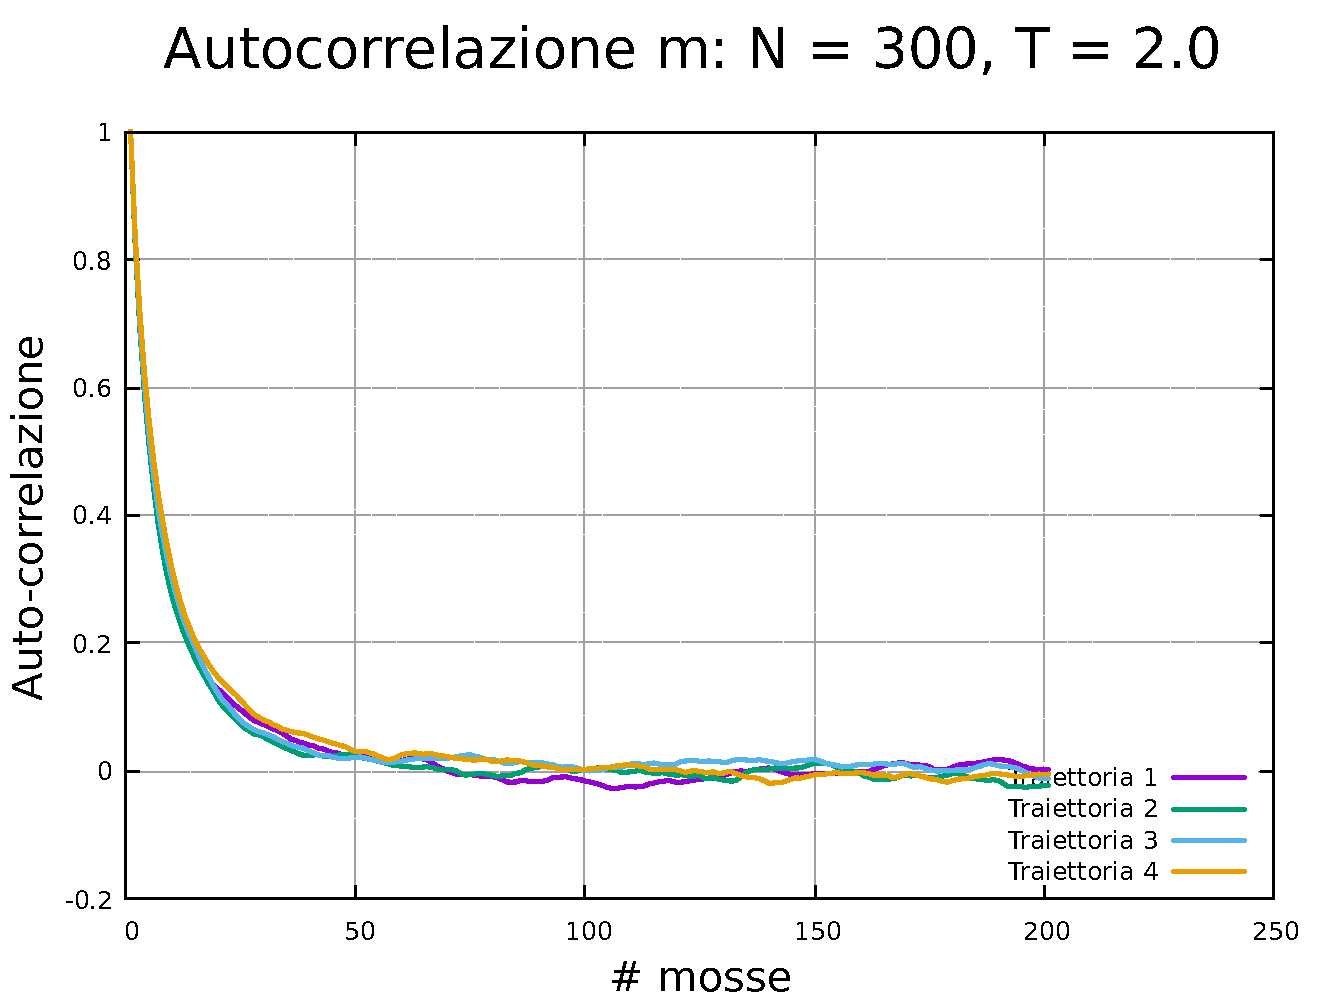
\includegraphics[page=1, width=\textwidth]{Immagini/simIsing2D/metro/tcorr/auto_300_2.0.pdf}
        \caption{$T\,=\,2.0$}
      \end{minipage}\hfill
      \begin{minipage}{0.45\textwidth}  
        \centering
        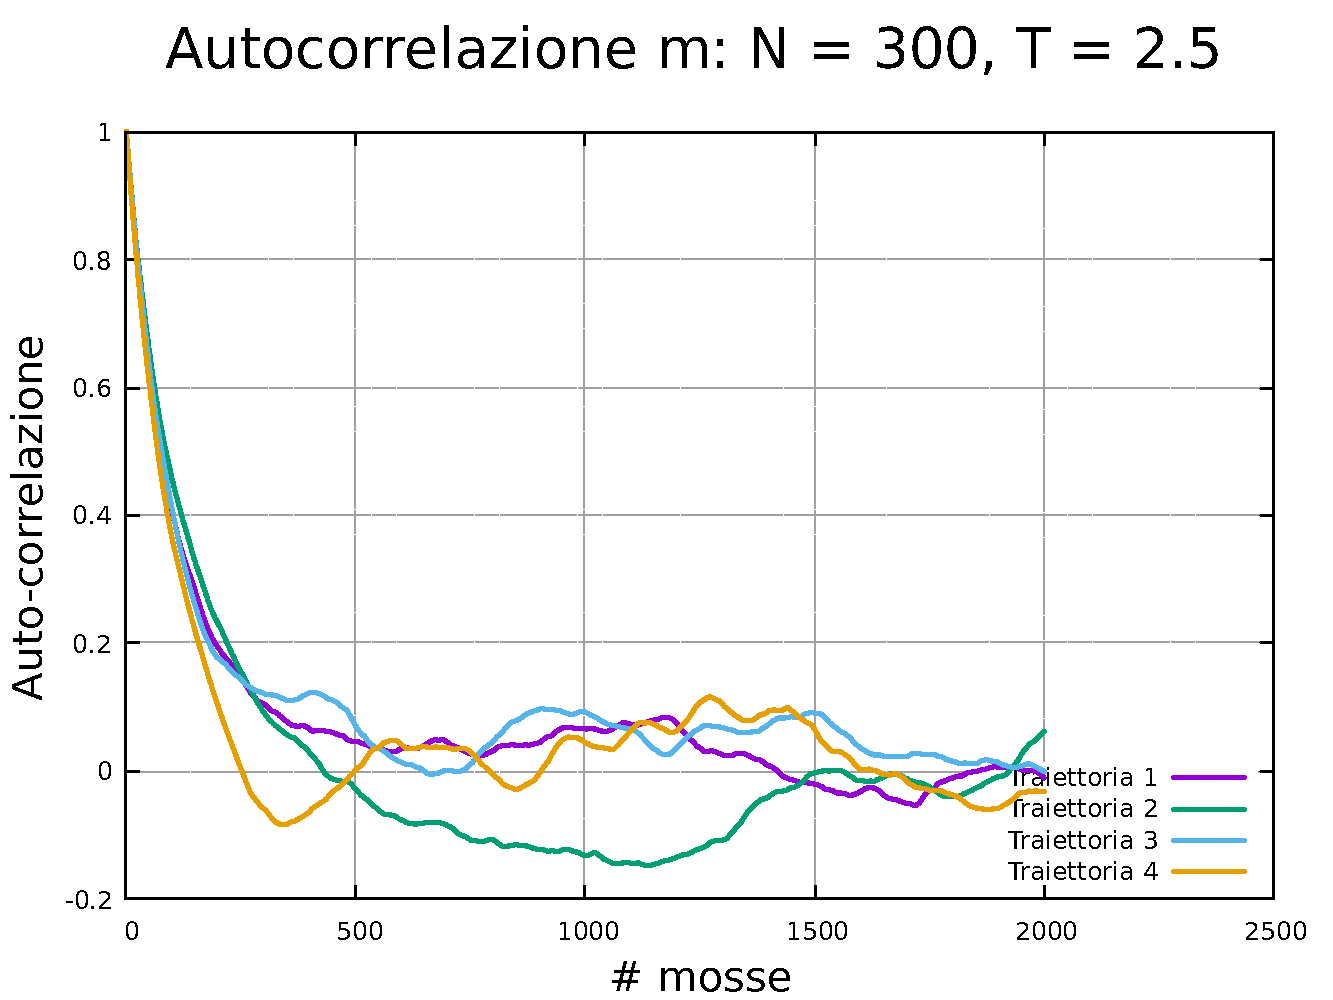
\includegraphics[page=1, width=\textwidth]{Immagini/simIsing2D/metro/tcorr/auto_300_2.5.pdf}
        \caption{$T\,=\,2.5$}
      \end{minipage}
    \vskip\baselineskip 
  
    \begin{minipage}{0.45\textwidth}  
      \centering
      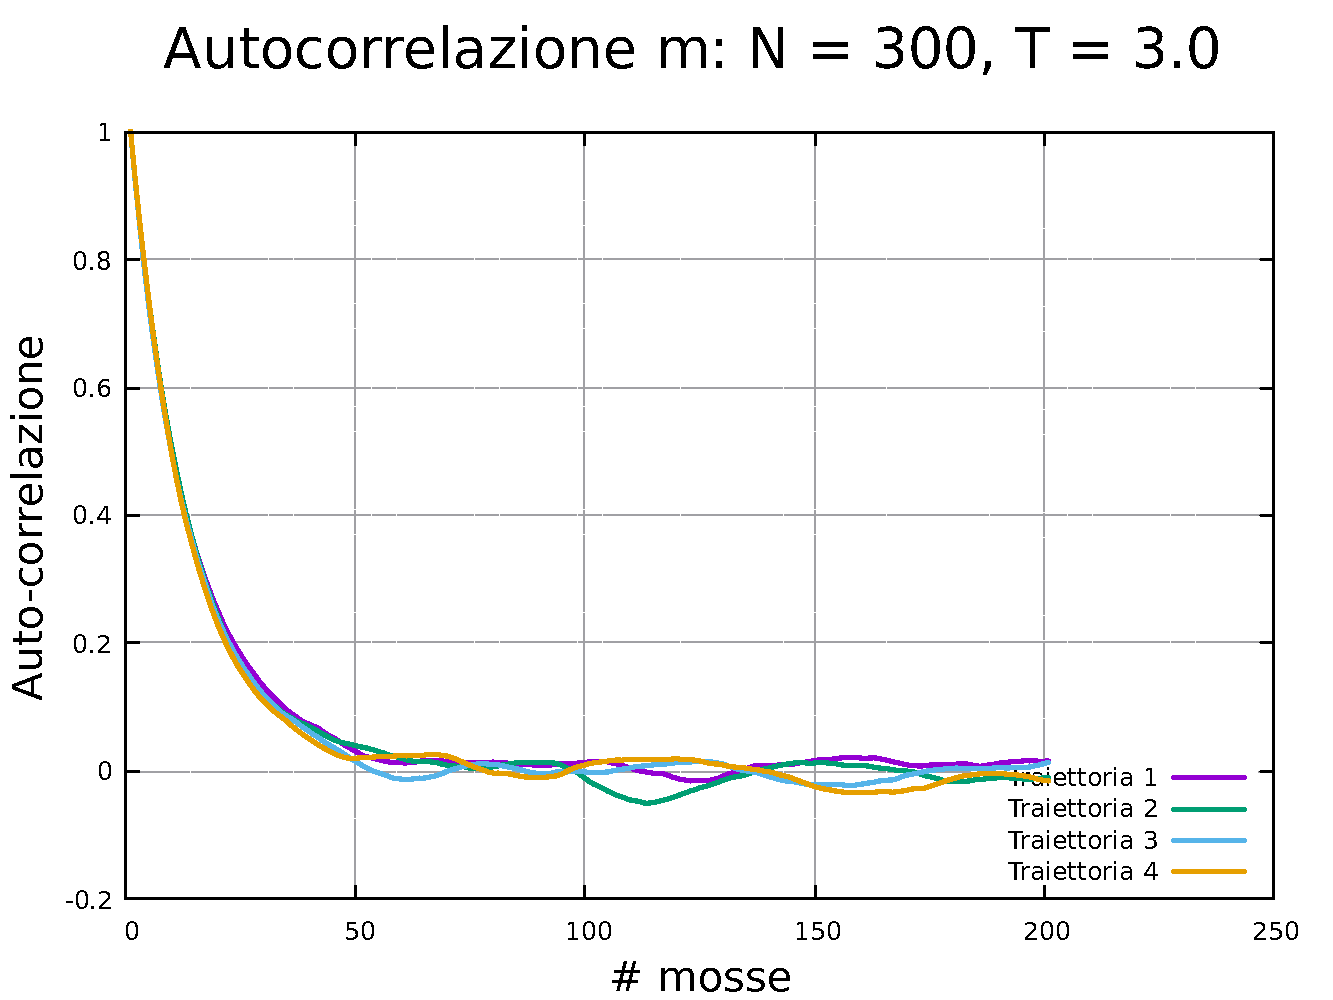
\includegraphics[page=1, width=\textwidth]{Immagini/simIsing2D/metro/tcorr/auto_300_3.0.pdf}
      \caption{$T\,=\,3.0$}
    \end{minipage}\hfill
    \begin{minipage}{0.45\textwidth}  
      \centering
      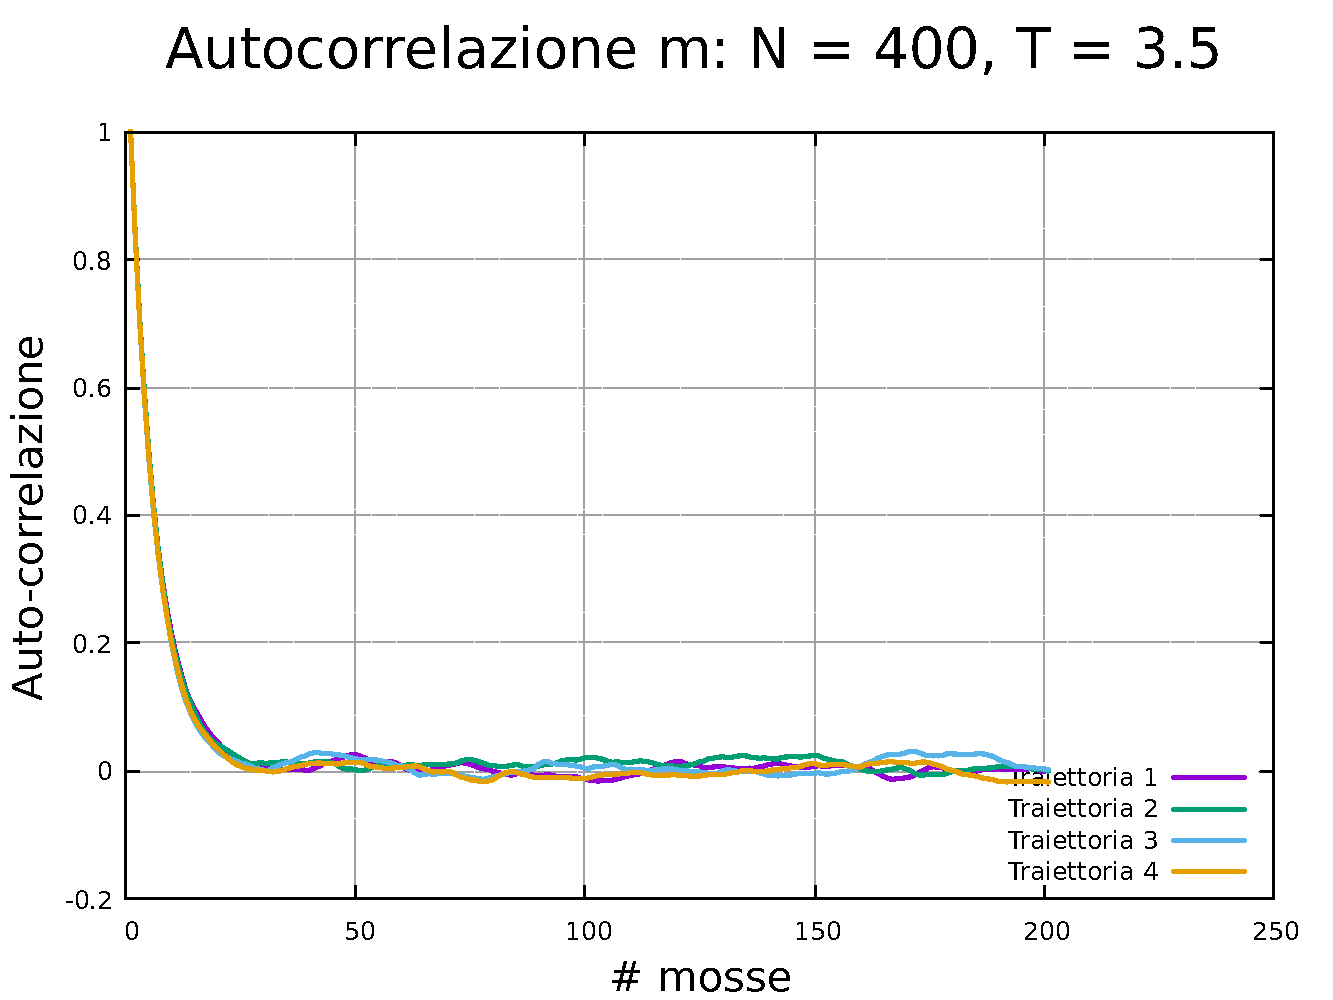
\includegraphics[page=1, width=\textwidth]{Immagini/simIsing2D/metro/tcorr/auto_300_3.5.pdf}
      \caption{$T\,=\,3.5$}
    \end{minipage}
    \caption{Studio dell'autocorrelazione di un modello di Ising 2D costituito da $300 \times 300$ spin.}
\end{figure}

\vspace*{\fill}



\vspace*{\fill}

\begin{figure}[H]
    \centering
    \begin{minipage}{0.45\textwidth}  
      \centering
      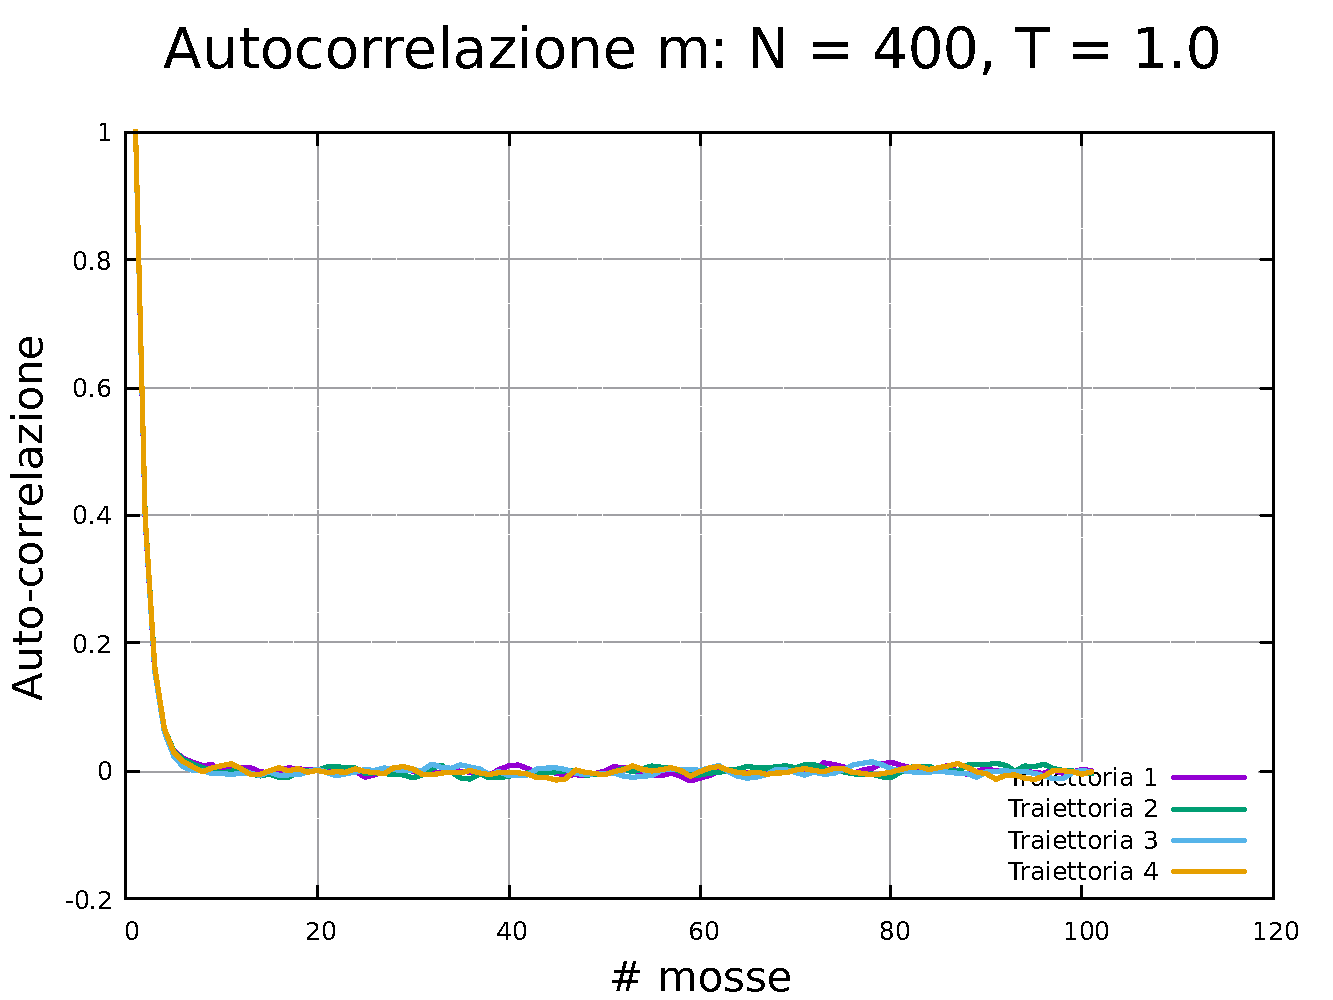
\includegraphics[page=1, width=\textwidth]{Immagini/simIsing2D/metro/tcorr/auto_400_1.0.pdf}
      \caption{$T\,=\,1.0$}
    \end{minipage}\hfill
    \begin{minipage}{0.45\textwidth}  
      \centering
      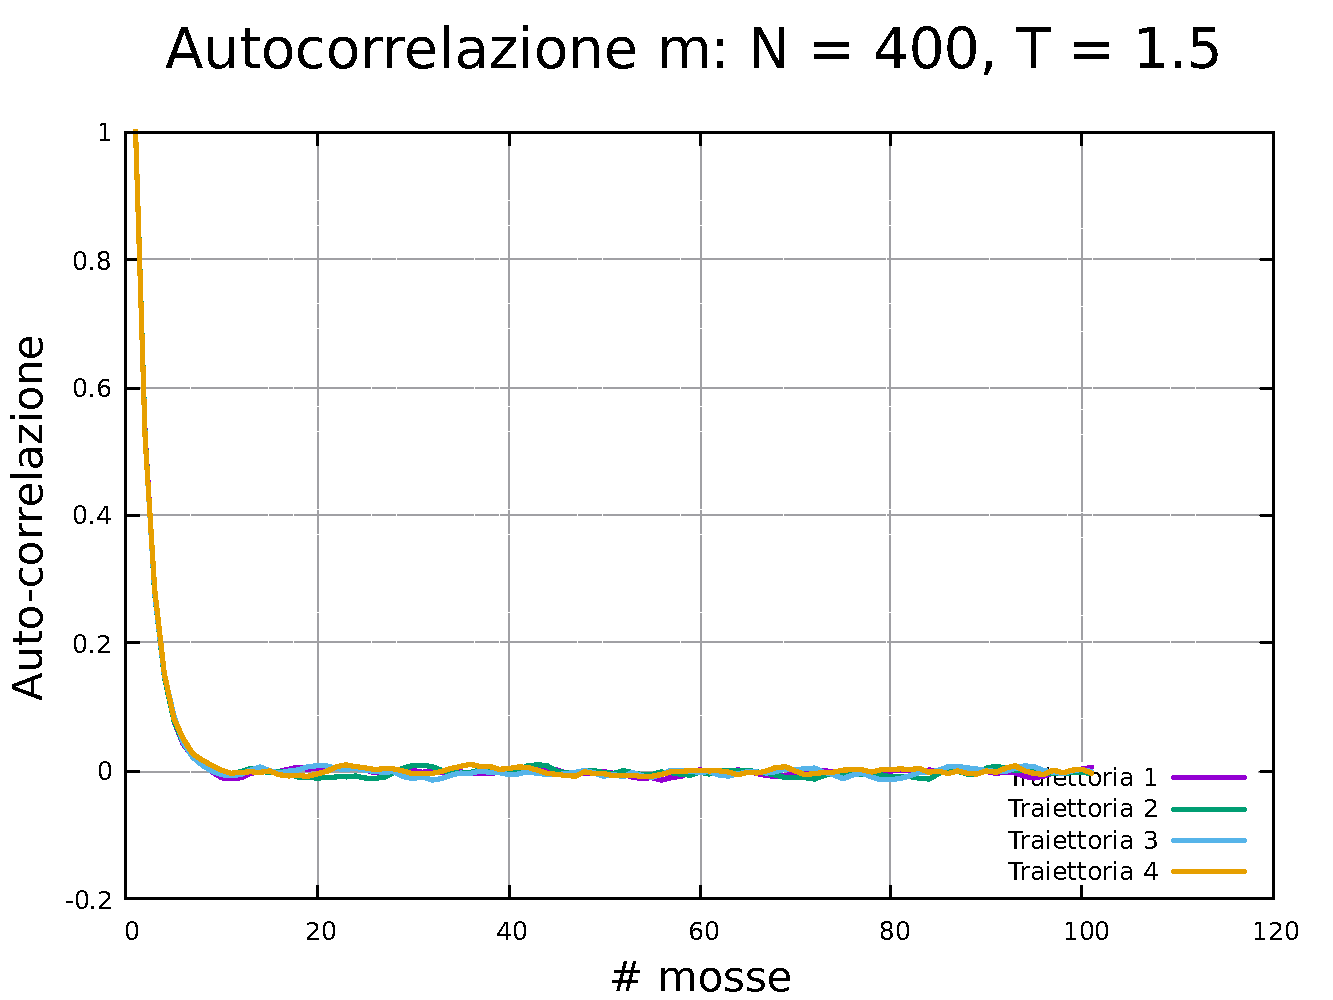
\includegraphics[page=1, width=\textwidth]{Immagini/simIsing2D/metro/tcorr/auto_400_1.5.pdf}
      \caption{$T\,=\,1.5$}
    \end{minipage}
    \vskip\baselineskip 

    \begin{minipage}{0.45\textwidth}  
        \centering
        \includegraphics[page=1, width=\textwidth]{Immagini/simIsing2D/metro/tcorr/auto_400_2.0.pdf}
        \caption{$T\,=\,2.0$}
      \end{minipage}\hfill
      \begin{minipage}{0.45\textwidth}  
        \centering
        \includegraphics[page=1, width=\textwidth]{Immagini/simIsing2D/metro/tcorr/auto_400_2.5.pdf}
        \caption{$T\,=\,2.5$}
      \end{minipage}
    \vskip\baselineskip 
  
    \begin{minipage}{0.45\textwidth}  
      \centering
      \includegraphics[page=1, width=\textwidth]{Immagini/simIsing2D/metro/tcorr/auto_400_3.0.pdf}
      \caption{$T\,=\,3.0$}
    \end{minipage}\hfill
    \begin{minipage}{0.45\textwidth}  
      \centering
      \includegraphics[page=1, width=\textwidth]{Immagini/simIsing2D/metro/tcorr/auto_400_3.5.pdf}
      \caption{$T\,=\,3.5$}
    \end{minipage}
    \caption{Studio dell'autocorrelazione di un modello di Ising 2D costituito da $400 \times 400$ spin.}
\end{figure}

\vspace*{\fill}



\vspace*{\fill}

\begin{figure}[H]
    \centering
    \begin{minipage}{0.45\textwidth}  
      \centering
      \includegraphics[page=1, width=\textwidth]{Immagini/simIsing2D/metro/tcorr/auto_500_1.0.pdf}
      \caption{$T\,=\,1.0$}
    \end{minipage}\hfill
    \begin{minipage}{0.45\textwidth}  
      \centering
      \includegraphics[page=1, width=\textwidth]{Immagini/simIsing2D/metro/tcorr/auto_500_1.5.pdf}
      \caption{$T\,=\,1.5$}
    \end{minipage}
    \vskip\baselineskip 

    \begin{minipage}{0.45\textwidth}  
        \centering
        \includegraphics[page=1, width=\textwidth]{Immagini/simIsing2D/metro/tcorr/auto_500_2.0.pdf}
        \caption{$T\,=\,2.0$}
      \end{minipage}\hfill
      \begin{minipage}{0.45\textwidth}  
        \centering
        \includegraphics[page=1, width=\textwidth]{Immagini/simIsing2D/metro/tcorr/auto_500_2.5.pdf}
        \caption{$T\,=\,2.5$}
      \end{minipage}
    \vskip\baselineskip 
  
    \begin{minipage}{0.45\textwidth}  
      \centering
      \includegraphics[page=1, width=\textwidth]{Immagini/simIsing2D/metro/tcorr/auto_500_3.0.pdf}
      \caption{$T\,=\,3.0$}
    \end{minipage}\hfill
    \begin{minipage}{0.45\textwidth}  
      \centering
      \includegraphics[page=1, width=\textwidth]{Immagini/simIsing2D/metro/tcorr/auto_500_3.5.pdf}
      \caption{$T\,=\,3.5$}
    \end{minipage}
    \caption{Studio dell'autocorrelazione di un modello di Ising 2D costituito da $500 \times 500$ spin.}
\end{figure}

\vspace*{\fill}














\subsection{Lunghezza dei blocchi}

\vspace*{\fill}
\begin{figure}[H]
    \centering
    \begin{minipage}{0.45\textwidth}  
      \centering
      \includegraphics[page=1, width=\textwidth]{Immagini/simIsing2D/metro/lblk/err_100_1.0.pdf}
      \caption{$T\,=\,1.0$}
    \end{minipage}\hfill
    \begin{minipage}{0.45\textwidth}  
      \centering
      \includegraphics[page=1, width=\textwidth]{Immagini/simIsing2D/metro/lblk/err_100_1.5.pdf}
      \caption{$T\,=\,1.5$}
    \end{minipage}
    \vskip\baselineskip 

    \begin{minipage}{0.45\textwidth}  
        \centering
        \includegraphics[page=1, width=\textwidth]{Immagini/simIsing2D/metro/lblk/err_100_2.0.pdf}
        \caption{$T\,=\,2.0$}
      \end{minipage}\hfill
      \begin{minipage}{0.45\textwidth}  
        \centering
        \includegraphics[page=1, width=\textwidth]{Immagini/simIsing2D/metro/lblk/err_100_2.5.pdf}
        \caption{$T\,=\,2.5$}
      \end{minipage}
    \vskip\baselineskip 
  
    \begin{minipage}{0.45\textwidth}  
      \centering
      \includegraphics[page=1, width=\textwidth]{Immagini/simIsing2D/metro/lblk/err_100_3.0.pdf}
      \caption{$T\,=\,3.0$}
    \end{minipage}\hfill
    \begin{minipage}{0.45\textwidth}  
      \centering
      \includegraphics[page=1, width=\textwidth]{Immagini/simIsing2D/metro/lblk/err_100_3.5.pdf}
      \caption{$T\,=\,3.5$}
    \end{minipage}
    \caption{Studio della lunghezza dei blocchi per un modello di Ising 2D costituito da $100 \times 100$ spin.}
\end{figure}

\vspace*{\fill}



\vspace*{\fill}

\begin{figure}[H]
    \centering
    \begin{minipage}{0.45\textwidth}  
      \centering
      \includegraphics[page=1, width=\textwidth]{Immagini/simIsing2D/metro/lblk/err_200_1.0.pdf}
      \caption{$T\,=\,1.0$}
    \end{minipage}\hfill
    \begin{minipage}{0.45\textwidth}  
      \centering
      \includegraphics[page=1, width=\textwidth]{Immagini/simIsing2D/metro/lblk/err_200_1.5.pdf}
      \caption{$T\,=\,1.5$}
    \end{minipage}
    \vskip\baselineskip 
  
    \begin{minipage}{0.45\textwidth}  
      \centering
      \includegraphics[page=1, width=\textwidth]{Immagini/simIsing2D/metro/lblk/err_200_2.0.pdf}
      \caption{$T\,=\,2.0$}
    \end{minipage}\hfill
    \begin{minipage}{0.45\textwidth}  
      \centering
      \includegraphics[page=1, width=\textwidth]{Immagini/simIsing2D/metro/lblk/err_200_2.5.pdf}
      \caption{$T\,=\,2.5$}
    \end{minipage}
    \vskip\baselineskip 

    \begin{minipage}{0.45\textwidth}  
        \centering
        \includegraphics[page=1, width=\textwidth]{Immagini/simIsing2D/metro/lblk/err_200_3.0.pdf}
        \caption{$T\,=\,3.0$}
      \end{minipage}\hfill
      \begin{minipage}{0.45\textwidth}  
        \centering
        \includegraphics[page=1, width=\textwidth]{Immagini/simIsing2D/metro/lblk/err_200_3.5.pdf}
        \caption{$T\,=\,3.5$}
    \end{minipage}

    \caption{Studio della lunghezza dei blocchi per un modello di Ising 2D costituito da $200 \times 200$ spin.}
\end{figure}

\vspace*{\fill}



\vspace*{\fill}

\begin{figure}[H]
    \centering
    \begin{minipage}{0.45\textwidth}  
      \centering
      \includegraphics[page=1, width=\textwidth]{Immagini/simIsing2D/metro/lblk/err_300_1.0.pdf}
      \caption{$T\,=\,1.0$}
    \end{minipage}\hfill
    \begin{minipage}{0.45\textwidth}  
      \centering
      \includegraphics[page=1, width=\textwidth]{Immagini/simIsing2D/metro/lblk/err_300_1.5.pdf}
      \caption{$T\,=\,1.5$}
    \end{minipage}
    \vskip\baselineskip 

    \begin{minipage}{0.45\textwidth}  
        \centering
        \includegraphics[page=1, width=\textwidth]{Immagini/simIsing2D/metro/lblk/err_300_2.0.pdf}
        \caption{$T\,=\,2.0$}
      \end{minipage}\hfill
      \begin{minipage}{0.45\textwidth}  
        \centering
        \includegraphics[page=1, width=\textwidth]{Immagini/simIsing2D/metro/lblk/err_300_2.5.pdf}
        \caption{$T\,=\,2.5$}
      \end{minipage}
    \vskip\baselineskip 
  
    \begin{minipage}{0.45\textwidth}  
      \centering
      \includegraphics[page=1, width=\textwidth]{Immagini/simIsing2D/metro/lblk/err_300_3.0.pdf}
      \caption{$T\,=\,3.0$}
    \end{minipage}\hfill
    \begin{minipage}{0.45\textwidth}  
      \centering
      \includegraphics[page=1, width=\textwidth]{Immagini/simIsing2D/metro/lblk/err_300_3.5.pdf}
      \caption{$T\,=\,3.5$}
    \end{minipage}
    \caption{Studio della lunghezza dei blocchi per un modello di Ising 2D costituito da $300 \times 300$ spin.}
\end{figure}

\vspace*{\fill}



\vspace*{\fill}

\begin{figure}[H]
    \centering
    \begin{minipage}{0.45\textwidth}  
      \centering
      \includegraphics[page=1, width=\textwidth]{Immagini/simIsing2D/metro/lblk/err_400_1.0.pdf}
      \caption{$T\,=\,1.0$}
    \end{minipage}\hfill
    \begin{minipage}{0.45\textwidth}  
      \centering
      \includegraphics[page=1, width=\textwidth]{Immagini/simIsing2D/metro/lblk/err_400_1.5.pdf}
      \caption{$T\,=\,1.5$}
    \end{minipage}
    \vskip\baselineskip 

    \begin{minipage}{0.45\textwidth}  
        \centering
        \includegraphics[page=1, width=\textwidth]{Immagini/simIsing2D/metro/lblk/err_400_2.0.pdf}
        \caption{$T\,=\,2.0$}
      \end{minipage}\hfill
      \begin{minipage}{0.45\textwidth}  
        \centering
        \includegraphics[page=1, width=\textwidth]{Immagini/simIsing2D/metro/lblk/err_400_2.5.pdf}
        \caption{$T\,=\,2.5$}
      \end{minipage}
    \vskip\baselineskip 
  
    \begin{minipage}{0.45\textwidth}  
      \centering
      \includegraphics[page=1, width=\textwidth]{Immagini/simIsing2D/metro/lblk/err_400_3.0.pdf}
      \caption{$T\,=\,3.0$}
    \end{minipage}\hfill
    \begin{minipage}{0.45\textwidth}  
      \centering
      \includegraphics[page=1, width=\textwidth]{Immagini/simIsing2D/metro/lblk/err_400_3.5.pdf}
      \caption{$T\,=\,3.5$}
    \end{minipage}
    \caption{Studio della lunghezza dei blocchi per un modello di Ising 2D costituito da $400 \times 400$ spin.}
\end{figure}

\vspace*{\fill}



\vspace*{\fill}

\begin{figure}[H]
    \centering
    \begin{minipage}{0.45\textwidth}  
      \centering
      \includegraphics[page=1, width=\textwidth]{Immagini/simIsing2D/metro/lblk/err_500_1.0.pdf}
      \caption{$T\,=\,1.0$}
    \end{minipage}\hfill
    \begin{minipage}{0.45\textwidth}  
      \centering
      \includegraphics[page=1, width=\textwidth]{Immagini/simIsing2D/metro/lblk/err_500_1.5.pdf}
      \caption{$T\,=\,1.5$}
    \end{minipage}
    \vskip\baselineskip 

    \begin{minipage}{0.45\textwidth}  
        \centering
        \includegraphics[page=1, width=\textwidth]{Immagini/simIsing2D/metro/lblk/err_500_2.0.pdf}
        \caption{$T\,=\,2.0$}
      \end{minipage}\hfill
      \begin{minipage}{0.45\textwidth}  
        \centering
        \includegraphics[page=1, width=\textwidth]{Immagini/simIsing2D/metro/lblk/err_500_2.5.pdf}
        \caption{$T\,=\,2.5$}
      \end{minipage}
    \vskip\baselineskip 
  
    \begin{minipage}{0.45\textwidth}  
      \centering
      \includegraphics[page=1, width=\textwidth]{Immagini/simIsing2D/metro/lblk/err_500_3.0.pdf}
      \caption{$T\,=\,3.0$}
    \end{minipage}\hfill
    \begin{minipage}{0.45\textwidth}  
      \centering
      \includegraphics[page=1, width=\textwidth]{Immagini/simIsing2D/metro/lblk/err_500_3.5.pdf}
      \caption{$T\,=\,3.5$}
    \end{minipage}
    \caption{Studio della lunghezza dei blocchi per un modello di Ising 2D costituito da $500 \times 500$ spin.}
\end{figure}

\vspace*{\fill}